\def\GRAPHPATH{localgraphics}

\ifdefined\HANDOUT
  \documentclass[handout,aspectratio=1610,dvipsnames]{beamer}
  \def\GRAPHPATH{graphics}
\else
  \documentclass[aspectratio=1610,dvipsnames]{beamer}
\fi

\usepackage[ngerman]{babel}
\usepackage{ifthen}
\usepackage{color}
\usepackage{colortbl}
\usepackage{textcomp}
\usepackage{multirow}
\usepackage{nicefrac}
\usepackage{multicol}
\usepackage{langsci-gb4e}
\usepackage{verbatim}
\usepackage{cancel}
\usepackage{graphicx}
\usepackage{hyperref}
\usepackage{verbatim}
\usepackage{boxedminipage}
\usepackage{adjustbox}
\usepackage{rotating}
\usepackage{booktabs}
\usepackage{bbding}
\usepackage{pifont}
\usepackage{multicol}
\usepackage{stmaryrd}
\usepackage{FiraSans}
\usepackage{soul}
\usepackage{tikz}
\usepackage{array}
\usepackage{xstring}

\usetikzlibrary{calc,decorations.pathmorphing,tikzmark,positioning,chains,trees,graphs,shapes,shadows,arrows}

\renewcommand\tikzmark[2]{%
  \tikz[remember picture,baseline=(chain-1.base),start chain] \node[on chain,inner sep=2pt,outer sep=0] (#1){#2};%
}

\newcommand\link[2]{%
  \begin{tikzpicture}[remember picture, overlay, >=stealth, shift={(0,0)}]
    \draw[-] (#1) --++(0,-12pt) -| (#2);
   \end{tikzpicture}%
}


\makeatletter
\g@addto@macro{\endtabular}{\rowfont{}}% Clear row font
\makeatother
\newcommand{\rowfonttype}{}% Current row font
\newcommand{\rowfont}[1]{% Set current row font
   \gdef\rowfonttype{#1}#1%
}
\newcolumntype{L}{>{\rowfonttype}l}


\usepackage{tikz-qtree}
\usepackage[linguistics]{forest}
\usepackage[maxbibnames=99,
  maxcitenames=2,
  uniquelist=false,
  backend=biber,
  doi=false,
  url=false,
  isbn=false,
  bibstyle=biblatex-sp-unified,
  citestyle=sp-authoryear-comp]{biblatex}

% Biblatex ============================================================

\addbibresource{rs.bib}

% Colors ==============================================================

\ifdefined\HANDOUT
  \definecolor{grau}{rgb}{0.5,0.5,0.5}
  \definecolor{lg}{rgb}{0.8,0.8,0.8}
  \definecolor{trueblue}{rgb}{0.3,0.3,1}
  \definecolor{ltb}{rgb}{0.8,0.8,1}
  \definecolor{lgr}{rgb}{0.5,1,0.5}
  \definecolor{orongsch}{RGB}{255,165,0}
  \definecolor{gruen}{rgb}{0,0.4,0}
  \definecolor{rot}{rgb}{0.7,0.2,0.0}
  \definecolor{tuerkis}{RGB}{63,136,143}
  \definecolor{braun}{RGB}{108,71,65}
  \definecolor{blaw}{rgb}{0,0,0.9}
\else
  \definecolor{grau}{rgb}{0.7,0.7,0.7}
  \definecolor{lg}{rgb}{0.9,0.9,0.9}
  \definecolor{trueblue}{rgb}{0.8,0.8,1}
  \definecolor{ltb}{rgb}{0.9,0.9,1}
  \definecolor{lgr}{rgb}{0.7,1,0.7}
  \definecolor{orongsch}{RGB}{255,200,100}
  \definecolor{gruen}{RGB}{0,230,0}
  \definecolor{rot}{RGB}{255,155,100}
  \definecolor{tuerkis}{RGB}{150,205,205}
  \definecolor{braun}{RGB}{140,120,115}
  \definecolor{blaw}{rgb}{0,0,0.9}
\fi

\newcommand{\gruen}[1]{\textcolor{gruen}{#1}}
\newcommand{\blaw}[1]{\textcolor{blaw}{#1}}
\newcommand{\rot}[1]{\textcolor{rot}{#1}}
\newcommand{\blau}[1]{\textcolor{trueblue}{#1}}
\newcommand{\orongsch}[1]{\textcolor{orongsch}{#1}}
\newcommand{\grau}[1]{\textcolor{grau}{#1}}
\newcommand{\whyte}[1]{\textcolor{white}{#1}}
\newcommand{\tuerkis}[1]{\textcolor{tuerkis}{#1}}
\newcommand{\braun}[1]{\textcolor{braun}{#1}}

% Newcommands =========================================================

\newcommand{\Dim}{\cellcolor{lg}}
\newcommand{\Dimblue}{\cellcolor{ltb}}
\newcommand{\Dimgreen}{\cellcolor{lgr}}
\newcommand{\Sub}[1]{\ensuremath{_{\text{#1}}}}
\newcommand{\Up}[1]{\ensuremath{^{\text{#1}}}}
\newcommand{\UpSub}[2]{\ensuremath{^{\text{#1}}_{\text{#2}}}}
\newcommand{\Spur}[1]{t\Sub{#1}}
\newcommand{\Ti}{\Spur{1}}
\newcommand{\Tii}{\Spur{2}}
\newcommand{\Tiii}{\Spur{3}}
\newcommand{\Tiv}{\Spur{4}}
\newcommand{\Ck}{\CheckmarkBold}
\newcommand{\Fl}{\XSolidBrush}
\newcommand{\xxx}{\hspaceThis{[}}
\newcommand{\zB}{z.\,B.\ }
\newcommand{\down}[1]{\ensuremath{\mathrm{#1}}}
\newcommand{\Zeile}{\vspace{\baselineskip}}
\newcommand{\Halbzeile}{\vspace{0.5\baselineskip}}
\newcommand{\Viertelzeile}{\vspace{0.25\baselineskip}}
\newcommand{\KTArr}[1]{\ding{222}~\fbox{#1}~\ding{222}}
\newcommand{\Ast}{*}
\newcommand{\SL}{\ensuremath{\llbracket}}
\newcommand{\SR}{\ensuremath{\rrbracket}}
\def\lspbottomrule{\bottomrule}
\def\lsptoprule{\toprule}
\newcommand{\Sw}[1]{\begin{sideways}#1\end{sideways}}
\newcommand{\Lab}{\ensuremath{\langle}}
\newcommand{\Rab}{\ensuremath{\rangle}}
\newcommand{\AbUmlautBreaker}{}
\ifdefined\HANDOUT
  \renewcommand{\AbUmlautBreaker}{\ /}
\fi
\newcommand{\LocStrutGrph}{\hspace{0.1\textwidth}}
\newcommand{\Nono}{---}

\newcommand{\Bewegtes}[1]{\ensuremath{_{\textrm{#1}}}}
\newcommand{\ORi}{\Bewegtes{1}}
\newcommand{\ORii}{\Bewegtes{2}}
\newcommand{\ORiii}{\Bewegtes{3}}
\newcommand{\ORiv}{\Bewegtes{4}}
\newcommand{\ORv}{\Bewegtes{5}}


% Beamer ==============================================================

\usetheme[hideothersubsections]{Boadilla}

\ifdefined\HANDOUT
  \usecolortheme{whale}
\else
  \usecolortheme{magpie}
\fi

\renewcommand<>{\rot}[1]{%
  \alt#2{\beameroriginal{\rot}{#1}}{#1}%
}
\renewcommand<>{\blau}[1]{%
  \alt#2{\beameroriginal{\blau}{#1}}{#1}%
}
\renewcommand<>{\orongsch}[1]{%
  \alt#2{\beameroriginal{\orongsch}{#1}}{#1}%
}
\renewcommand<>{\gruen}[1]{%
  \alt#2{\beameroriginal{\gruen}{#1}}{#1}%
}

\setbeamercolor{alerted text}{fg=trueblue}

\newcounter{lastpagemainpart}

\resetcounteronoverlays{exx}

\AtBeginSection[]{
  \begingroup
  \setbeamertemplate{navigation symbols}{}
  \begin{frame}[noframenumbering,plain]
  \vfill
  \centering
  \begin{beamercolorbox}[sep=8pt,center,shadow=true,rounded=true]{title}
    \usebeamerfont{title}\insertsectionhead\par%
  \end{beamercolorbox}
  \vfill
  \end{frame}
  \endgroup
}

\setbeamertemplate{itemize item}[circle]
\setbeamertemplate{enumerate item}[square]

\setbeamertemplate{navigation symbols}{\insertframenumber/\inserttotalframenumber\hspace{5em}}

% Tikz ================================================================

\usetikzlibrary{positioning,arrows,cd}
\tikzset{>=latex}

% Forest

\forestset{
  Ephr/.style={draw, ellipse, thick, inner sep=2pt},
  Eobl/.style={draw, rounded corners, inner sep=5pt},
  Eopt/.style={draw, rounded corners, densely dashed, inner sep=5pt},
  Erec/.style={draw, rounded corners, double, inner sep=5pt},
  Eoptrec/.style={draw, rounded corners, densely dashed, double, inner sep=5pt},
  Ehd/.style={rounded corners, fill=gray, inner sep=5pt,
    delay={content=\whyte{##1}}
  },
  Emult/.style={for children={no edge}, for tree={l sep=0pt}},
  phrasenschema/.style={for tree={l sep=2em, s sep=2em}},
  decide/.style={draw, chamfered rectangle, inner sep=2pt},
  finall/.style={rounded corners, fill=gray, text=white},
  intrme/.style={draw, rounded corners},
  yes/.style={edge label={node[near end, above, sloped, font=\scriptsize]{Ja}}},
  no/.style={edge label={node[near end, above, sloped, font=\scriptsize]{Nein}}},
  sake/.style={tier=preterminal},
  ake/.style={
    tier=preterminal
    },
}

\tikzset{
    invisible/.style={opacity=0,text opacity=0},
    visible on/.style={alt=#1{}{invisible}},
    alt/.code args={<#1>#2#3}{%
      \alt<#1>{\pgfkeysalso{#2}}{\pgfkeysalso{#3}}
    },
}

\forestset{
  visible on/.style={
    for tree={
      /tikz/visible on={#1},
      edge+={/tikz/visible on={#1}}}}}

\useforestlibrary{edges}

\forestset{
  narroof/.style={roof, inner xsep=-0.25em, rounded corners},
  forky/.style={forked edge, fork sep-=7.5pt},
  bluetree/.style={for tree={trueblue}, for children={edge=trueblue}},
  orongschtree/.style={for tree={orongsch}, for children={edge=orongsch}},
  rottree/.style={for tree={rot}, for children={edge=rot}},
  gruentree/.style={for tree={gruen}, for children={edge=gruen}},
  tuerkistree/.style={for tree={tuerkis}, for children={edge=tuerkis}},
  brauntree/.style={for tree={braun}, for children={edge=braun}},
  grautree/.style={for tree={grau}, for children={edge=grau}}, 
  gruennode/.style={gruen, edge=gruen},
  graunode/.style={grau, edge=grau},
}


% Drawing sonority diagrams =========================================== 

\makeatletter

\long\def\ifnodedefined#1#2#3{%
  \@ifundefined{pgf@sh@ns@#1}{#3}{#2}}

\newcommand\aeundefinenode[1]{%
  \expandafter\ifx\csname pgf@sh@ns@#1\endcsname\relax
  \else
    \typeout{Undefining node "#1"}%
    \global\expandafter\let\csname pgf@sh@ns@#1\endcsname\relax
  \fi
}

\newcommand\aeundefinethesenodes[1]{%
  \foreach \myn  in {#1}
    {%
      \ifnodedefined{\myn}{%
      \expandafter\aeundefinenode\expandafter{\myn}%
    }{}
    }%
}

\newcommand\aeundefinenumericnodes{%
  \foreach \myn in {1,2,...,50}
    {%
      \ifnodedefined{\myn}{%
      \expandafter\aeundefinenode\expandafter{\myn}%
    }{}
    }%
}
\makeatother

\newcommand{\plo}{0}
\newcommand{\fri}{0.5}
\newcommand{\nas}{1}
\newcommand{\liq}{1.5}
\newcommand{\vok}{2}

% Save text.
\newcommand{\lastsaved}{}
\newcommand{\textsave}[1]{\gdef\lastsaved{#1}#1}

\newcommand{\SonDiag}[2][0]{%
  \begin{tikzpicture}
    \textsave{.}
    \tikzset{
      normalseg/.style={fill=white},
      extrasyll/.style={circle, draw, fill=white},
      sylljoint/.style={diamond, draw, fill=white}
    }
    \node at (0,\plo) {P};
    \node at (0,\fri) {F};
    \node at (0,\nas) {N};
    \node at (0,\liq) {L};
    \node at (0,\vok) {V};

    % Draw the helper lines if required.
    \ifthenelse{\equal{#1}{0}}{}{%
      \foreach \y in {\plo, \fri, \nas, \liq,\vok} {%
	\draw [dotted, |-|] (0.25, \y) -- (#1.75, \y);
      }
    }

    \foreach [count=\x from 1, remember=\x as \lastx] \p / \y / \g in #2 {
      \ifthenelse{\equal{\y}{-1}}{\textsave{.}}{%

	% Draw the node, either plain, as Silbenbgelenk, or as extrasyllabic.
        \ifthenelse{\equal{\g}{1}}{%
	  \node (\x) [sylljoint] at (\x, \y) {\p};
	}{%
	  \ifthenelse{\equal{\g}{2}}{%
	    \node (\x) [extrasyll] at (\x, \y) {\p};
	  }{%
	    \node (\x) [normalseg] at (\x, \y) {\p};
	  }
	}

	% Draw the connection unless the previous node was not or was empty.
	\ifthenelse{\NOT\equal{\lastsaved}{.}}{%
	  \draw [->] (\lastx) to (\x);
	}{}
	\textsave{1}
      }
    }
    \aeundefinenumericnodes
  \end{tikzpicture}
}


\setbeamertemplate{navigation symbols}{}
\setbeamertemplate{section in toc}[circle]
\setbeamertemplate{subsection in toc}[square]
\setbeamertemplate{subsubsection in toc}[triangle]

\setbeamerfont{section in toc}{size=\tiny}
\setbeamerfont{subsection in toc}{size=\tiny}



\ifdefined\TITLE
  \title[Statistik]{Statistik\\\StrSubstitute{\TITLE}{+}{ }}
\else
  \title[Statistik]{Statistik}
\fi

\author{Roland Schäfer}
\institute[FSU Jena]{Institut für Germanistische Sprachwissenschaft\\Friedrich-Schiller-Universität Jena}

\ifdefined\TITLE
  \date[\StrSubstitute{\TITLE}{+}{ }]{\grau{stets aktuelle Fassungen: \url{https://github.com/rsling/VL-Deutsche-Syntax}}}
\else
  \date[Kompletter Foliensatz]{\grau{stets aktuelle Fassungen: \url{https://github.com/rsling/VL-Deutsche-Syntax}}}
\fi

\begin{document}

\begingroup
  \setbeamertemplate{navigation symbols}{}
  \begin{frame}[noframenumbering,plain]
   \titlepage
  \end{frame}

  \begin{frame}{Inhalt}
    \centering 
    \scalebox{0.9}{\begin{minipage}{\textwidth}
      \begin{multicols}{2}
        \tableofcontents
      \end{multicols}
    \end{minipage}}
    \end{frame}
\endgroup

\ifdefined\TITLE
  \input{includes/\TITLE}
\else
  \section{Inferenz}
  \let\woopsi\section\let\section\subsection\let\subsection\subsubsection
  
\section{Probative Wissenschaft}

\begin{frame}
  {Empirisch, objektiv, realistisch, exakt(?)}
  \begin{itemize}[<+->]
    \item \alert{Beobachtbare} Phänomene
    \item Beobachtungen \alert{reproduzierbar}
    \item Messbar = beobachtbar (Sinneswahrnehmung an sich irrelevant)
      \Zeile
    \item \alert{Realismus} | wirkliche Phänomene und ihre Mechanismen
    \item \orongsch{Keine postmoderne Realitäts- und Objektivitätsverweigerung}
      \Zeile
    \item \alert{Kontrolliertes Experiment}
  \end{itemize}
\end{frame}

\begin{frame}
  {Empirie | Gründe für Reproduzierbarkeitsbedingung}
  \begin{itemize}[<+->]
    \item Intrinsische Ungenauigkeiten der Messung (\alert{Wirkung} plus \orongsch{Störeinflüsse})
    \item Potentiell inadäquate Messung des theoretischen Konstrukts
      \Halbzeile
    \item[→] Vermeidung von Fehlschluss auf unechte Ursachen
    \item[→] \alert{Relevante Ursachen}
      \Halbzeile
    \item[→] Insgesamt \alert{Stärkung der Validität}
  \end{itemize}
\end{frame}

\begin{frame}
  {Beispiel | Fehlgeleitete Generative Grammatiker}
  \begin{itemize}[<+->]
    \item Gegenstand: interne (mentale) Grammatik (I-Grammatik)\\
      universeller und individueller Teil
    \item I-Grammatik bei jedem Sprecher (leicht) verschieden
    \item I-Grammatik erlaubt immer binäre Grammatikalitätsentscheidung
      \Halbzeile
    \item[→] \orongsch{Linguisten können eigene I-Grammatik untersuchen (Introspektion)!}
  \end{itemize}
  \Zeile
  \onslide<+->
  \centering 
  \rot{Das Ergebnis ist die aktuelle Krise der Linguistik.}
\end{frame}


\begin{frame}
  {Inferenz I | Positivismus und Induktion}
  \onslide<+->
  \onslide<+->
  \begin{block}
    {(Logischer) Positivismus}
    \alert{Formale} Ableitung von Wissen (= Theorien) aus Beobachtbarem und irgendeiner Logik. \alert{Induktion}. Keine Metaphysik. Keine Kreativität erwünscht. \grau{(\citealt{Carnap1928}, \ldots)} 
  \end{block}
  \Zeile
  \onslide<+->
  Aber suchen wir wirklich nur nach \alert{Mustern}, \zB in Korpusdaten?\\
    \Halbzeile
    \begin{itemize}[<+->]
      \item Was ist der \alert{zugrundeliegende Mechanismus}?
      \item Wie kommen wir zu \alert{erklärenden Theorien} von Mustern in Daten?
      \item \alert{Datenaufbereitung} (\zB im Korpus) kann dann nicht theoriegeleitet sein.
        \Halbzeile
      \item \orongsch{Die ART folgt auch nicht einfach so aus Daten!}
    \end{itemize}
\end{frame}

\begin{frame}
  {Inferenz II | Rationalistischer Probativismus (Falsifikationismus)}
  \onslide<+->
  \onslide<+->
  \begin{block}
    {Rationalistischer Probativismus}
    Theorien werden aufgestellt von \alert{Menschen, die die Welt beobachten}. Theorien werden \alert{getestet an Daten}, aber nicht logisch aus Daten abgeleitet. Wissenschaft lernt aus Fehlern. \grau{(\citealt{Popper1962,Mayo1996}, \ldots)}
  \end{block}
  \onslide<+->
  \Zeile
  Unter dieser Philosophie werden plötzlich Dinge wichtig \ldots
    \Halbzeile
    \begin{itemize}[<+->]
      \item Ist eine \alert{Stichprobe repräsentativ} für das, was man zeigen will?
      \item Welche \alert{Methode der statistischen Analyse} wird verwendet?
      \item Für eine Korpusstudie muss die Datenaufbereitung damit theoriegeleitet sein!
      \item Liefert die Studie \alert{\textit{a serious Argument from Error}}?\\
        \onslide<+->
        \Halbzeile
        {\small\textit{There is evidence an error is absent to the extent that a \alert{procedure with\\
        a very high capability of signalling the error}, if and only if it is present,\\
      nevertheless detects no error.} \grau{\citep[16]{Mayo2018}}}\\
    \end{itemize}
\end{frame}



\begin{frame}
  {Hypothesen}
  Die konkrete Hypothesen, die in einem Experiment getestet werden,\\
  sind \orongsch{nie} die Primärhypothesen der Theorie.
  \Zeile
  \begin{itemize}[<+->]  
    \item \alert{Abgeleitete Partikularhypothesen} über konkrete Erwartungen im Experiment
    \item Einfluss zahlreicher \alert{Auxiliarhypothesen}, \zB über Messprozeduren
    \item[ ] \grau{\citet{Duhem1914,Quine1951,Laudan1990}}
    \Zeile
    \item "`Interessante"' Hypothesen
      \begin{itemize}[<+->]
        \item Formulierung relevanter \alert{Kausationsbedingung} (wenn, dann)
        \item \alert{Universelle Gültigkeit} | ein Sprecher vs.\ alle Sprecher
        \item Also \zB\ \orongsch{uninteressant} | \textit{Welchen Kasus nimmt wegen?}
      \end{itemize}
      \Halbzeile
  \end{itemize}
\end{frame}

\begin{frame}
  {Hypothesenprüfung | Probativismus (Falsifikationismus)}
  \begin{center}
    \alert{Kann die Hypothese weiter angenommen werden,\\
    oder liefert das Experiment starke Evidenz gegen sie?}
  \end{center}
  \Zeile
  \begin{itemize}[<+->]
    \item Probleme bei Prüfung
      \Viertelzeile
      \begin{itemize}[<+->]
        \item Falsch abgeleitete Partikularhypothese
        \item Falsche Sekundärhypothesen
	\item Störeinflüsse, intrinsische Messungenauigkeit
        \item Mangelhafte \alert{Operationalisierung}
	\item Zu wenige Daten (oder zu viele Daten?)
      \end{itemize}
  \end{itemize}
\end{frame}


\section{Elemente der Empirie}

\begin{frame}
  {Grundgesamtheit}
  \begin{itemize}[<+->]
    \item Von Interesse | \alert{allgemeine Gesetzmäßigkeiten}
    \item Also Untersuchungsgegenstand: \alert{alle x} (Sprecher, Sätze, \dots)
    \item Untersuchbar | kleine Menge von x
  \end{itemize}
  \Zeile
  \centering 
  \alert{Grundgesamtheit} | alle x\\
  \Viertelzeile
  \alert{Datengenerierender Prozess (DGP)} | Prozess, der \alert{alle x} hervorbringt\\
  \Zeile
  \alert{Stichprobe} | eine kleine Menge x, aus der auf Grundgesamtheit\\
  bzw.\ DGP geschlossen werden soll
\end{frame}

\begin{frame}
  {Stichprobe}
    \begin{block}{Uniform zufällige Stichprobe}
      Jedes Element der Grundgesamtheit hat die gleiche Chance beim Ziehen.
    \end{block}
    \Zeile
    \begin{block}{Stratifizierte Stichprobe}
      Die Stichprobe ist so zusammengesetzt, dass wichtige Eigenschaften proportional repräsentiert sind.
    \end{block}
    \Zeile
  \begin{itemize}
    \item Problem bei Letzterem: haufenweise Auxiliarhypothesen
  \end{itemize}
\end{frame}

\begin{frame}
  {Operationalisierung und Auxiliarhypothesen}
  \begin{itemize}[<+->]
    \item \alert{Operationalisierung} | präzise Formulierung der Messmethode\\
      für ein theoretisches Konstrukt
      \Zeile
    \item Bsp.\ Konstrukt "`Satzlänge"': Wortanzahl? Phonemanzahl? Phrasenanzahl?
    \item Bsp.\ Konstrukt "`Satztopik"': Oha!?! \citep{CookBildhauer2013}
      \Zeile
    \item Alle genannten Beispiele \alert{abhängig von Auxiliarhypothesen}\\
      bzw.\ anderen theoretischen Konstrukten (Wort, Phonem, Phrase, \dots)
  \end{itemize}
\end{frame}

\begin{frame}
  {Variablen I}
  \begin{itemize}[<+->]
    \item Uninteressanter Typ Fragestellung | "`Wieviel Prozent X haben Eigenschaft A?"'
    \item \orongsch{Fehlen jeglicher Aussagen über kausale Zusammenhänge}
    \item Bsp.\ | Wie oft wird \textit{wegen} mit Dat bzw.\ Gen verwendet?
      \Halbzeile
    \item Besser | "`Wie bedingt Eigenschaft B die Wahrscheinlichkeit von A bei X?"'
    \item Bsp.\ | Per Hypothese nehmen denominale Präpositionen eher den Gen als den Dat.
  \end{itemize}
  \pause
  \Halbzeile
  \begin{center}
    Konzeptionell:
    \scalebox{0.7}{
      \begin{tabular}[h!]{|c||c|c|}
	\cline{2-3}
	\multicolumn{1}{c||}{} & denominale P & andere P \\
	\hline
	\hline
	Dat & $x_1$ & $x_2$\\
	\hline
	Gen & $x_3$ & $x_4$\\
	\hline
      \end{tabular}
    }
  \end{center}
\end{frame}

\begin{frame}
  {Variablen II}
  Operationalisierte und gemessene Eigenschaften sind \alert{Variablen}.\\
  \Zeile
  \begin{itemize}[<+->]
    \item Im Experiment:
      \Halbzeile
      \begin{itemize}[<+->]
	\item \alert{Kontrolliere} für Theorie irrelevante Variablen (\alert{Störvariablen})\\
          bzw.\ verlass dich auf deren Zufallsverteilung (Fisher, s.\,u.).
          \Viertelzeile
	\item \alert{Variiere} "`Ursachen-Variablen"' (\alert{unabhängige Variablen}).
          \Viertelzeile
	\item \alert{Beobachte} "`Wirkung-Variablen"' (\alert{abhängige Variablen}).
      \end{itemize}
  \end{itemize}
\end{frame}

\begin{frame}
  {Experiment und Quasi-Experiment}
  \begin{itemize}[<+->]
    \item Problem in Astronomie, Korpuslinguistik usw. | keine Experimente möglich
    \item \alert{Unabhängige Variablen nicht variierbar}
    \item Daten liegen bereits vor bzw.\ fallen vom Himmel
    \item Auswahl von Datensätzen, so dass von den unabhängigen Variablen\\
      die zur Theorieprüfung nötigen Permutationen im Datensatz vorkommen
    \item Dabei Zusatzproblem bei Korpuslinguistik: Korpus meist nicht\\
      das eigene, wenig Informationen über mögliche Verzerrungen
      \Zeile
    \item \alert{Was ist die Grundgesamtheit bzw.\ der DGP?}
  \end{itemize}
\end{frame}


\section{Validität}

\begin{frame}
  {Statistische Validität}
  Gefahren für \orongsch{statistische Schlussverfahren}\\
  \Zeile
  \begin{itemize}[<+->]
    \item \alert{Falsches Testverfahren} für die gegebene Situation
    \item \alert{Mathematische Vorbedingungen} für das Testverfahren nicht
    \item \alert{Zu viele Partikulartests} einer übergeordneten Hypothese aus denselben Daten
    \item Zu \alert{kleine Stichprobe}
    \item Zu \alert{große Stichprobe}
    \item Zu große Variation in der Grundgesamtheit
  \end{itemize}
\end{frame}

\begin{frame}
  {Interne Validität}
  \begin{itemize}[<+->]
    \item Irrtum beim \orongsch{Herstellen des Kausalzusammenhangs}
    \Zeile
    \item Fiktives Bsp.:
     \Halbzeile 
      \begin{itemize}[<+->]
        \item Korpora | DWDS-Kernkorpus enthält Texte 1900--2000, DECOW12 Texte nach 2000
          \Viertelzeile
	\item Hypothese | Im DECOW12 kommt öfter das Pronomen \textit{son} vor als im\\
          DWDS Kernkorpus, weil es erst nach 2000 zum eigenständigen Pronomen wurde.
          \Viertelzeile
	\item Die Hypothese wird bestätigt anhand von Stichproben aus den beiden Korpora.
          \Viertelzeile
        \item \rot{Die wirkliche Ursache sind aber Registerunterschiede}.
      \end{itemize}
  \end{itemize}
\end{frame}

\begin{frame}
  {Validität des Konstrukts}
  \begin{itemize}[<+->]
    \item Korrektheit des \alert{theoretischen Konstrukts}
      \Zeile
    \item Eigentlich aus der Psychologie
    \item Aber riesiges Problem in der Linguistik
      \Zeile
    \item Echtes Bsp.
      \Viertelzeile
      \begin{itemize}
	\item Beobachtung | Das Deutsche bewahrt genus-typische Pluralflexion am Substantiv.
	\item Konstrukt | Nominalklammer\slash Klammerprinzip (NP-Kongruenzklammer Art -- Subst)\\
          \grau{\citep{Ronneberger2010}}
	\item Hypothese (post-hoc zur Beobachtung) | Flexionserhalt stärkt Klammerprinzip
          \Halbzeile
	\item \rot{Das Konstrukt ist hochgradig beliebig und unterdefiniert, damit nicht testbar.}
         \Halbzeile 
	\item \alert{Abhilfe: nur Konstrukte\slash Hypothesen, die starke Vorhersagen generieren}
      \end{itemize}
  \end{itemize}
\end{frame}

\begin{frame}
  {Externe Validität}
  \begin{itemize}[<+->]
    \item \alert{Generalisierbarkeit der Ergebnisse} (über Raum, Zeit usw.)
      \Zeile
    \item Problem | \alert{zu große Homogenität der Stichprobe}\\
      (was für statistische Validität wiederum gut ist)
      \Halbzeile
    \item Bezug auf Korpora:
      \begin{itemize}[<+->]
	\item Zu spezifische Stratifikation (DeReKo)
	\item Verzerrte Stichprobe (Webkorpora)
      \end{itemize}
  \end{itemize}
\end{frame}

\section{Ronald A.\ Fisher, Wahrscheinlichkeit, Ereignisraum, Teetassen}

\begin{frame}
  {Ronald A.\ Fisher (1890--1962)}
  \begin{itemize}[<+->]
    \item Statistik als Teil der rationalen wissenschaftlichen Argumentation,\\
      der Interpretation von Experimenten
      \Viertelzeile
    \item Möglichst kein Mathematik-Jargon, eher intuitiv zugängliche\\
      mathematische Konzepte
      \Halbzeile
    \item \orongsch{Eingeschränkte statistische Inferenz als theoriegeleitete Dateninterpretation}
      \Halbzeile
    \item Kontrolle aller unabhängigen Variablen
    \item \alert{Alle anderen (Stör-)Variablen konzeptuell zufallsgebunden}
  \end{itemize}
\end{frame}

\begin{frame}
  {The Tea-Tasting Lady}
  Muriel Bristow behauptet, sie könne am Geschmack einer Tasse Tee erkennen,\\
  ob die Milch oder der Tee zuerst eingeschenkt wurde. Fisher führt\\
  ein Experiment durch (acht Tassen, vier mit dem Tee zuerst) und fragt,\\
  wie wir entscheiden können, ob das Ergebnis davon zeugt, dass sie\\
  diese Fähigkeit wirklich hat.\\
  \Halbzeile
  \begin{itemize}[<+->]
    \item \gruen{Liegt das Ergebnis \orongsch{deutlich} über dem per Zufall erwartbaren Niveau?}
      \Halbzeile
    \item Idee vor Fisher | \alert{alle Störvariablen kontrollieren}\\
      und gleich machen, dann ist induktive Inferenz möglich 
    \item Fisher | Das ist prinzipiell unmöglich, umständlich, teuer und \alert{unnötig}!
      \Halbzeile
    \item Wenn alle irrelevanten Störvariablen zufallsverteilt sind, dann gilt:
      \Viertelzeile
      \begin{itemize}[<+->]
	\item Variiere die relevante unabhängige Variable.
          \Viertelzeile
        \item Vergleiche das Ergebnis mit \alert{zufällig erwartbaren Ergebnissen}.
      \end{itemize}
  \end{itemize}
\end{frame}

\begin{frame}
  {Wahrscheinlichkeit}
  Bayesische Wahrscheinlichkeit (\textit{inverse probability)}\\
  \begin{itemize}[<+->]
    \item \rot{Für wie wahrscheinlich hält Individuum I das Ereignis E?}
    \item Subjektiv, berücksichtigt vorherige Überzeugung
    \item Aktualisierung von Überzeugungen
    \item Basiert auf \alert{Bayes Rule} (Tomas Bayes 1763)
    \item \alert{Ereignisraum} (s.\,u.) irrelevant!
  \end{itemize}
  \Zeile
  Frequentistische Wahrscheinlichkeit\\
  \begin{itemize}[<+->]
    \item \alert{Wie viele mögliche Ereignisse e\Sub{i} aus E treten ein?}
    \item Zu jedem Experiment gehört ein \alert{Ereignisraum} (s.\,u.)!
    \item Daher \alert{objektiv}, unabhängig von Überzeugungen
    \item \alert{Wenn ein Ereignis e\Sub{i} eingetreten ist, wird seine Wahrscheinlichkeit uninteressant.}
    \item Geeignet für rationalistisch-probativistische Wissenschaftsphilosophie
  \end{itemize}
\end{frame}

\begin{frame}
  {Frequentismus | Ereignisraum (sample space)}
  Für ein Experiment gilt:\\
  \Halbzeile
  \begin{itemize}[<+->]
    \item Wir beobachten \alert{$n$ Messungen} (Stichprobe),\\
      jede Messung wird aus einer \alert{definierten Menge von möglichen Messungen}.
      \Halbzeile
      \begin{itemize}[<+->]
        \item Bsp. | 10 Mal einen Würfel werfen \{1, 2, 3, 4, 5, 6\}.
          \Viertelzeile
        \item Bsp. | Je 10 Akzeptabilitätsurteile unter 2 Bedingungen von 100 Probanden \{Ja, Nein\}.
      \end{itemize}
      \Zeile
    \item Wir bekommen ein \alert{konkretes Ergebnis}.
      \Halbzeile
      \begin{itemize}[<+->]
        \item Bsp. | 8 von 10 Würfen mehr als drei Augen.
          \Viertelzeile
        \item Bsp. | "`Mehr"' Ja-Antworten unter Bedingung A (schon deutlich komplexeres Design).
      \end{itemize}
      \Halbzeile
    \item Wir müssen berücksichtigen, \alert{wie viele Ergebnisse (und welche) es insgesamt\\
      hätte geben können}, um zu bewerten, wie unwahrscheinlich das Ergebnis \rot{war}.
      \Viertelzeile
    \item \alert{Ereignisraum (sample space)} | Menge der möglichen Ausgänge des Experiments
  \end{itemize}
\end{frame}

\begin{frame}
  {Warum "`\rot{war}"'?}
  \grau{Wir müssen berücksichtigen, wie viele Ergebnisse (und welche) es insgesamt\\
    hätte geben können, um zu bewerten, wie unwahrscheinlich das Ergebnis \rot{war}.}\\
    \Zeile
    \begin{itemize}[<+->]
      \item Jedes eingetretene Ereignis hat die Wahrscheinlichkeit 1.
        \Halbzeile
        \begin{itemize}[<+->]
          \item Die Wahrscheinlichkeit, dass Helmut Kohl 1998 abgewählt wurde, ist 1.
            \Viertelzeile
          \item Die Wahrscheinlichkeit, dass wir 8 Würfe mit mehr als drei Augen hatten, ist 1.
        \end{itemize}
      \Halbzeile
      \item \rot{Nach dem Experiment} | P(konkreter Ausgang des Experiments wurde erzielt) = 1
      \item \gruen{Vor dem Experiment} | P(konkreter Ausgang des Experiments wird erzielt werden) < 1
    \end{itemize}
    \Zeile
    \centering 
    \orongsch{Die übelsten Fehler in der Bewertung statistischer Ergebnisse rühren daher,\\
    dass Menschen diese Sachverhalte vergessen.}\\
\end{frame}

\begin{frame}
  {Zurück zur Tea-Tasting Lady}
  \alert{Design des Experiments} | Muriel Bristow probiert \alert{acht Tassen},\\
  (vier mit Milch zuerst, vier mit Tee zuerst) und \alert{wählt die vier mit Tee zuerst aus}.\\
  \Zeile
  \begin{itemize}[<+->]
    \item \alert{Mit wie vielen richtigen Treffern wären Sie zufrieden?}
      \Halbzeile
    \item Es muss die \alert{frequentistische Wahrscheinlichkeit} errechnet werden,\\
      eine, zwei, drei oder vier Tassen auch \orongsch{per Zufall} richtig zu raten.
      \Halbzeile
    \item Dann können wir beurteilen, ob das Ergebnis\\
      \textit{\orongsch{deutlich} \gruen{über dem erwartbaren Niveau}} liegt.
  \end{itemize}
\end{frame}

\begin{frame}
  {Ausgang 1 | Alle vier Tassen korrekt}
  Allgemein:\\
  \Viertelzeile
  \begin{equation}
    P(\mathsf{konkreter\ Ausgang})=\frac{\gruen{\mathsf{Anzahl\ richtiger\ Zuweisungen}}}{\alert{\mathsf{Anzahl\ aller\ potentiellen\ Zuweisungen}}}
  \end{equation}\\
  \Zeile
  Für diesen Ausgang:\\
  \Viertelzeile
  \begin{equation}
    P(\mathsf{vier\ Tassen\ korrekt})=\frac{\gruen{1}}{\alert{\mathsf{Anzahl\ aller\ potentiellen\ Zuweisungen}}}
  \end{equation}
\end{frame}

\begin{frame}
  {Wie viele Möglichkeiten gibt es?}
  Wir wählen \alert{vier \textit{Tee zuerst}-Tassen (TZ) aus acht Tassen} aus:\\
  \Halbzeile
  \begin{itemize}[<+->]
    \item erste TZ-Tasse: eine von 8 (bleiben 7)
    \item zweite TZ-Tasse: eine von 7 (bleiben 6)
    \item dritte TZ-Tasse: eine von 6 (bleiben 5)
    \item vierte TZ-Tasse: eine von 5 (bleiben 4)
      \Halbzeile
    \item[→] \rot{STOPP} | alle anderen 4 Tassen automatisch MZ
  \end{itemize}
  \Zeile
  \centering 
  Also naiv gedacht | \alert{$8\cdot7\cdot6\cdot5=1680$}
\end{frame}

\begin{frame}
  {Die Reihenfolge}
  \orongsch{1680 ist zu hoch}, denn je nachdem, welche Tasse aus den verbleibenden wir wählen,\\
  ergeben sich \orongsch{andere Permutationen (Reihenfolgen) desselben Ergebnisses}.\\
  \Zeile
  \begin{itemize}[<+->]
    \item Bsp. | Auswahl von Tasse 7, 3, 6, 1 identisch zu 3, 1, 6, 7 usw.
      \Halbzeile
    \item Es gibt von jeder möglichen Auswahl gleich viele Permutationen.
    \item Und zwar die Anzahl der \alert{Möglichkeiten, vier Tassen zu ordnen: $4\cdot3\cdot2\cdot1$}
      \Zeile
  \end{itemize}
  \Zeile
  \begin{equation}
    \mathsf{Anzahl\ aller\ potentiellen\ Zuweisungen}=\frac{8\cdot7\cdot6\cdot5}{4\cdot3\cdot2\cdot1}=\frac{1680}{24}=70
  \end{equation}
\end{frame}

\begin{frame}
  {Wenn sie also genau richtig liegt \ldots}
  Wahrscheinlichkeit, per Zufall genau richtig zu liegen:\\
  \Viertelzeile
  \begin{equation}
    P(\mathsf{vier\ Tassen\ korrekt})=\frac{\gruen{1}}{\alert{70}}=0.014
  \end{equation}\\
  \Zeile
  \centering 
  \blau{Interpretieren Sie das Ergebnis.}
\end{frame}

\begin{frame}
  {Für die Generalisierung der Berechnung}
  \begin{itemize}[<+->]
    \item Eigentlich haben wir es mit \alert{Binomialkoeffizienten} zu tun.
      \Halbzeile
    \item "`Lotto-Kombinationen"' | $k$ aus $n$\\
      \alert{ohne Zurücklegen und ohne Beachtung der Reihenfolge}
  \end{itemize}
  \Zeile
  \pause
  \begin{equation}
    \binom{n}{k}=\frac{n!}{k!(n-k)!}
  \end{equation}
\end{frame}

\begin{frame}
  {Ausgang 2 | Drei Tassen korrekt}
  Berechnung mit dem Binomialkoeffizienten
  \Halbzeile
  \begin{itemize}[<+->]
    \item Die drei richtigen aus vier TZ| \gruen{$\binom{4}{3}$}
    \item Die eine falsche aus vier TZ | \rot{$\binom{4}{1}$}
  \end{itemize}
  \Zeile
  \pause
  \begin{equation}
    P(drei\ richtig\ per\ Zufall)=\frac{\gruen{\binom{4}{3}}\cdot\rot{\binom{4}{1}}}{70}=\frac{16}{70}=\alert{0.229}
  \end{equation}\\
  \Zeile
  \centering 
  \blau{Interpretieren Sie das Ergebnis.}
\end{frame}

\begin{frame}
  {Darstellung als Kreuztabelle}
  \centering 
  \alert{Ausgang 1}\\
  \begin{tabular}[h]{rrcc}
    \toprule
    && \multicolumn{2}{c}{\textbf{Realität}} \\
    && \textbf{Tee zuerst} & \textbf{Milch zuerst} \\
    \midrule
    \multirow{2}{*}{\textbf{Lady}} & \textbf{Tee zuerst} & 4 & 0 \\
    & \textbf{Milch zuerst} & 0 & 4 \\
    \bottomrule
  \end{tabular}\\
  \vspace{2\baselineskip}
  \alert{Ausgang 2}\\
  \begin{tabular}[h]{rrcc}
    \toprule
    && \multicolumn{2}{c}{\textbf{Realität}} \\
    && \textbf{Tee zuerst} & \textbf{Milch zuerst} \\
    \midrule
    \multirow{2}{*}{\textbf{Lady}} & \textbf{Tee zuerst} & 3 & 1 \\
    & \textbf{Milch zuerst} & 1 & 3 \\
    \bottomrule
  \end{tabular}
\end{frame}

\begin{frame}
  {Stichprobengröße und Effektstärke}
  \begin{itemize}[<+->]
    \item Unbefriedigendes Ergebnis bei 3 von 4 richtigen Tassen
      \Halbzeile
    \item Sehr \orongsch{kleine Stichprobe} | nur perfektes Ergebnis zufriedenstellend
    \item \orongsch{Effektstärke} | Vielleicht kann MB ca.\ 75 \% aller Tassen richtig erkennen.
  \end{itemize}
  \Zeile
  \centering 
  Bei größerer Stichprobe | Was ist mit \alert{30 von 40 richtigen Tassen},\\also insgesamt 80 Tassen?\\
  \Halbzeile
  Das wäre die \alert{gleiche Effektstärke}, aber eine \alert{größere Stichprobe}.
\end{frame}

\begin{frame}
  {Letzte Warnung}
  Was zeigt man mit so einem Experiment? Und was nicht?\\
  \Zeile
  \begin{itemize}[<+->]
    \item Der Ausgang \rot{war} \gruen{ziemlich unwahrscheinlich},\\
      bevor das Experiment durchgeführt wurde.
    \item Daher gehen wir bis auf Weiteres davon aus, \gruen{dass ein Effekt vorliegt} \ldots
    \item \ldots\ \rot{oder zufällig ein seltenes Ereignis eingetreten ist!!!}
      \Halbzeile
    \item Wenn Sie mit den Geburtsdaten Ihrer Familie im Lotto gewinnen,\\
      \rot{ist ein seltenes Ereignis eingetreten}, Sie haben aber \rot{nicht gezeigt,\\
      dass Ihre Geburtsdaten die Lottokugeln beeinflussen}!
      \Halbzeile
    \item \alert{Ein solches Ergebnis beweist also nichts!}
    \item Die Logik basiert auf der Annahme einer wiederholten Testung.
    \item[→] Wenn wir das Experiment \alert{sehr oft} machen, und es gibt \alert{keinen Effekt},\\
      dann nähert sich die \alert{Verteilung der Ergebnisse der Zufallsverteilung} an.
  \end{itemize}
\end{frame}

\ifdefined\TITLE
  \section{Nächste Woche | Überblick}
  \begin{frame}
    {Einzelthemen}
    \begin{enumerate}
      \item Inferenz 
      \item \alert{Deskriptive Statistik}
      \item Nichtparametrische Verfahren
      \item z-Test und t-Test
      \item ANOVA
      \item Freiheitsgrade und Effektstärken
      \item Power und Severity
      \item Lineare Modelle
      \item Generalisierte Lineare Modelle
      \item Gemischte Modelle
    \end{enumerate}
  \end{frame}
\fi


  \let\subsection\section\let\section\woopsi

  \section{Deskriptive Statistik}
  \let\woopsi\section\let\section\subsection\let\subsection\subsubsection
  
\begin{frame}
  {Übersicht}
  \begin{itemize}[<+->]
    \item Deskriptive Statistik als \alert{Aggregation von Daten}
      \Halbzeile
    \item Verteilungen in Stichproben und Grundgesamtheiten:
      \begin{itemize}
	\item Zentralmaße
	\item Streuung (Varianz)
      \end{itemize}
    \item \orongsch{Theoretische vs.\ empirische Verteilungen}
      \Halbzeile
    \item \alert{Konfidenzintervalle} | Genauigkeiten von Schätzungen?
  \end{itemize}
\end{frame}

\begin{frame}
  {Literatur}
  \begin{itemize}
    \item Google, Stackoverflow usw.
      \Zeile
    \item \citet{GravetterWallnau2007}\\
      Achtung! \orongsch{Vermittelt eine falsche Philosophie bei Anwendung der Tests!}
      \Halbzeile
    \item \citet{Bortz2010}
  \end{itemize}
\end{frame}

\section{Motivation}

\begin{frame}
  {Zweck der deskriptiven Statistik}
  \begin{itemize}[<+->]
    \item Mit unbewaffnetem Auge auf Daten zu blicken, ist meistens zwecklos.
      \Halbzeile
    \item In Zahlen sehen Menschen nur schlecht Tendenzen und Zusammanhänge.
      \Zeile
    \item Deskriptive Statistik
      \begin{itemize}[<+->]
        \item \alert{Zusammenfassen}
        \item \alert{Gruppieren}
        \item \alert{Visualisieren}
      \end{itemize}
  \end{itemize}
\end{frame}


\begin{frame}
  {Was will man wissen?}
  \begin{itemize}[<+->]
    \item Definition der Grundgesamtheit
      \Halbzeile
    \item \alert{Stichprobengröße ($n$)}
      \begin{itemize}[<+->]
        \item 200 Sätze aus dem Korpus
        \item 1.000 Reaktionen (von 50 Probanden) im Experiment
        \item Was sind die elementaren gemessenen Datenpunkte?
      \end{itemize}
      \Halbzeile
    \item Stichprobenmethode
      \begin{itemize}[<+->]
        \item \alert{Zufallsstichprobe} | Nachweis der uniformen Zufälligkeit
        \item \alert{Quotenstichprobe} | Stratifzierung und Begründung
      \end{itemize}
  \end{itemize}
\end{frame}


\section{Skalenniveau}

\begin{frame}
  {Messvariablen und Skalenniveaus}
  \begin{itemize}[<+->]
    \item \alert{dichotom\slash binär} | \gruen{Menge $\{A, B\}$} | zwei disjunkte Kategorien\\
      \grau{männlich, weiblich ; Präteritum, Perfekt}
      \Viertelzeile
    \item \alert{nominal\slash kategorial} | \gruen{Menge $\{A, B, ..\}$} | disjunkte Kategorien\\
      \grau{Parteizugehörigkeit ; NP, AP, VP}
      \Viertelzeile
    \item \alert{ordinal} | \gruen{Tupel $\langle A, B, ..\rangle$, \rot{nicht} $\mathbb{N}$ oder $\mathbb{Z}$} | disjunkte Kategorien mit Rang\\
      \grau{Schulnoten ; 5- oder 7-Punkt-Skalen für Akzeptabilität}\\
      \Viertelzeile
    \item \alert{Verhältnis} | \gruen{$+\mathbb{Q}_0$} | geordnete Werte mit Nullpunkt\\
      \grau{Temperatur in Kelvin ; Lesezeiten}
      \Viertelzeile
    \item \alert{Intervall} | \gruen{$\mathbb{Q}$} | Wie Verhältnis, aber ohne Nullpunkt\\
      \grau{Temperatur in Celsius}
      \Zeile
    \item \rot{Zähldaten} | \rot{Keine} beobachtbaren Variablen, sondern\\
      Aggregation von dichtotomen, nominalen oder ordinalen Variablen\\
  \end{itemize}
\end{frame}

\begin{frame}
  {Intervalle vs.\ Verhältnisse}
  \begin{itemize}[<+->]
    \item \alert{Verhältnisskala} | Größe von Menschen in cm
      \begin{itemize}[<+->]
	\item $200 cm = 2 \times 100 cm$ usw.
	\item Keine Messung unter $0 cm$ 
      \end{itemize}
      \Zeile
    \item \alert{Intervallskala} | Dasselbe als \alert{Abweichung vom Mittel}
      \begin{itemize}[<+->]
	\item $4 cm = 2 \times 2 cm$ usw.
        \item \orongsch{$184 cm \neq 2 \times 182 cm$}
	\item Negative Messungen möglich
      \end{itemize}
  \end{itemize}
\end{frame}

\begin{frame}
  {Relevanz der Skalenniveaus}
  \begin{itemize}[<+->]
    \item Bestimmung \alert{zulässiger mathematischer Operationen}
      \Halbzeile
    \item \alert{Deskriptive Statistiken} je nach Skalenniveau
      \Halbzeile
    \item Zulässigkeit von \alert{inferenzstatistischen Tests} je nach Skalenniveau
  \end{itemize}
\end{frame}


\section{Zentraltendenz}

\begin{frame}
  {Zentraltendenz I}
  \alert{Modus} | Der \alert{häufigste Wert} | \orongsch{Alle Skalenniveaus}\\
  \Zeile
  \begin{center}
    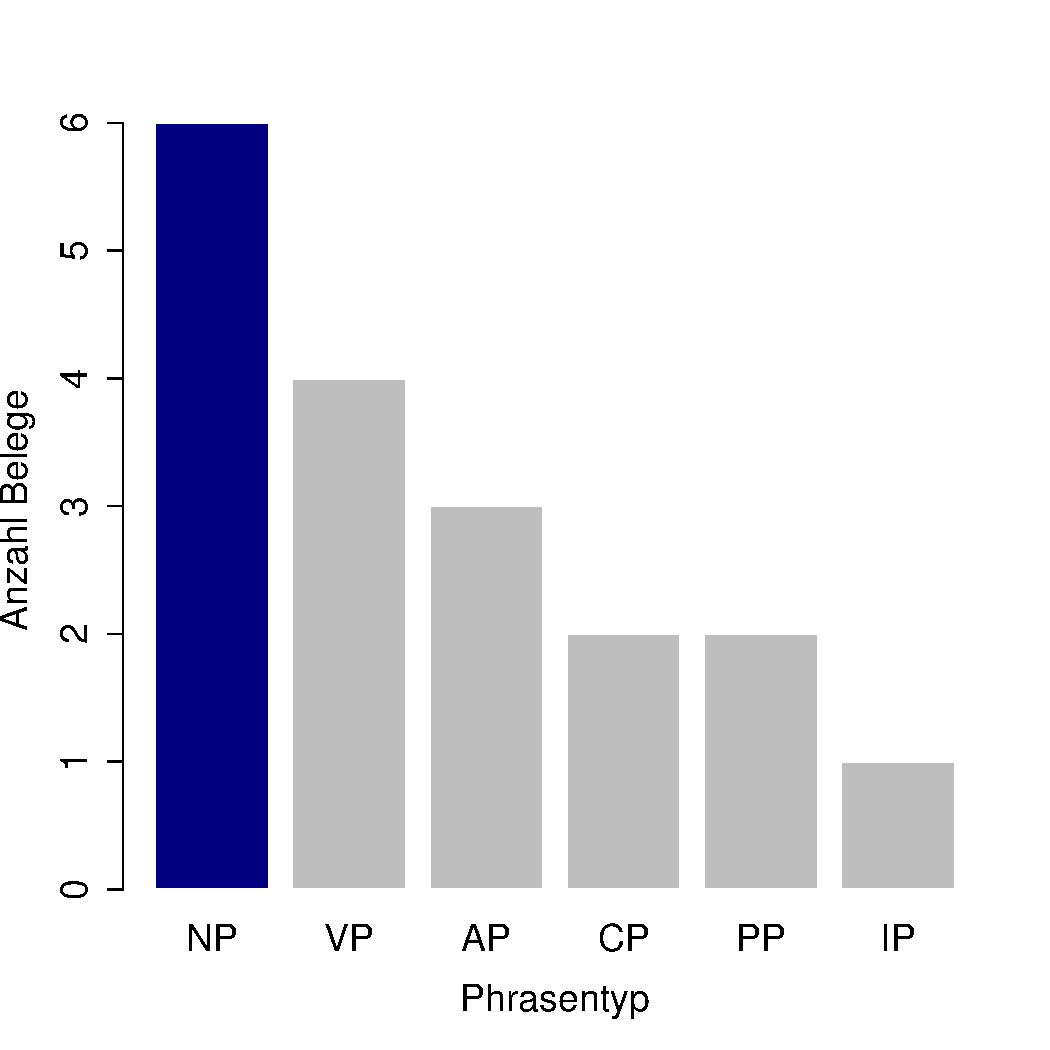
\includegraphics[height=0.6\textheight]{RVorlesung/mode}
  \end{center}
\end{frame}

\begin{frame}
  {Zentraltendenz II}
  \alert{Median} | \alert{Mitte der sortierten Stichprobe} | \orongsch{ab Ordinalskala}\\
  \Zeile
  \begin{center}
    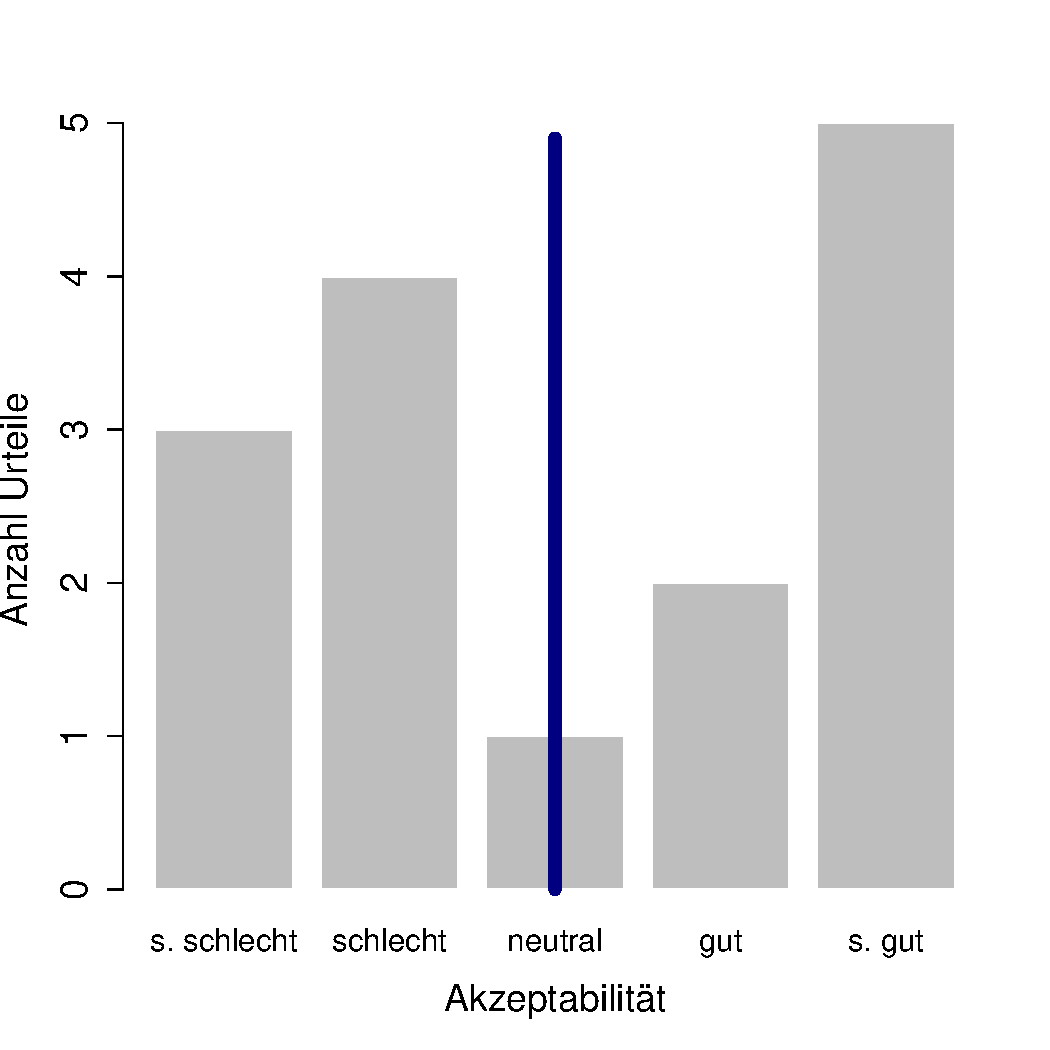
\includegraphics[height=0.6\textheight]{RVorlesung/median}
  \end{center}
  \Zeile
  \grau{\footnotesize Numerische Messungen | Verschiedene Interpolationsmethoden\\
    \url{https://en.wikipedia.org/wiki/Quantile\#Estimating_quantiles_from_a_sample}}
\end{frame}

\begin{frame}
  {Median bestimmen | Stichprobe}
  \centering 
  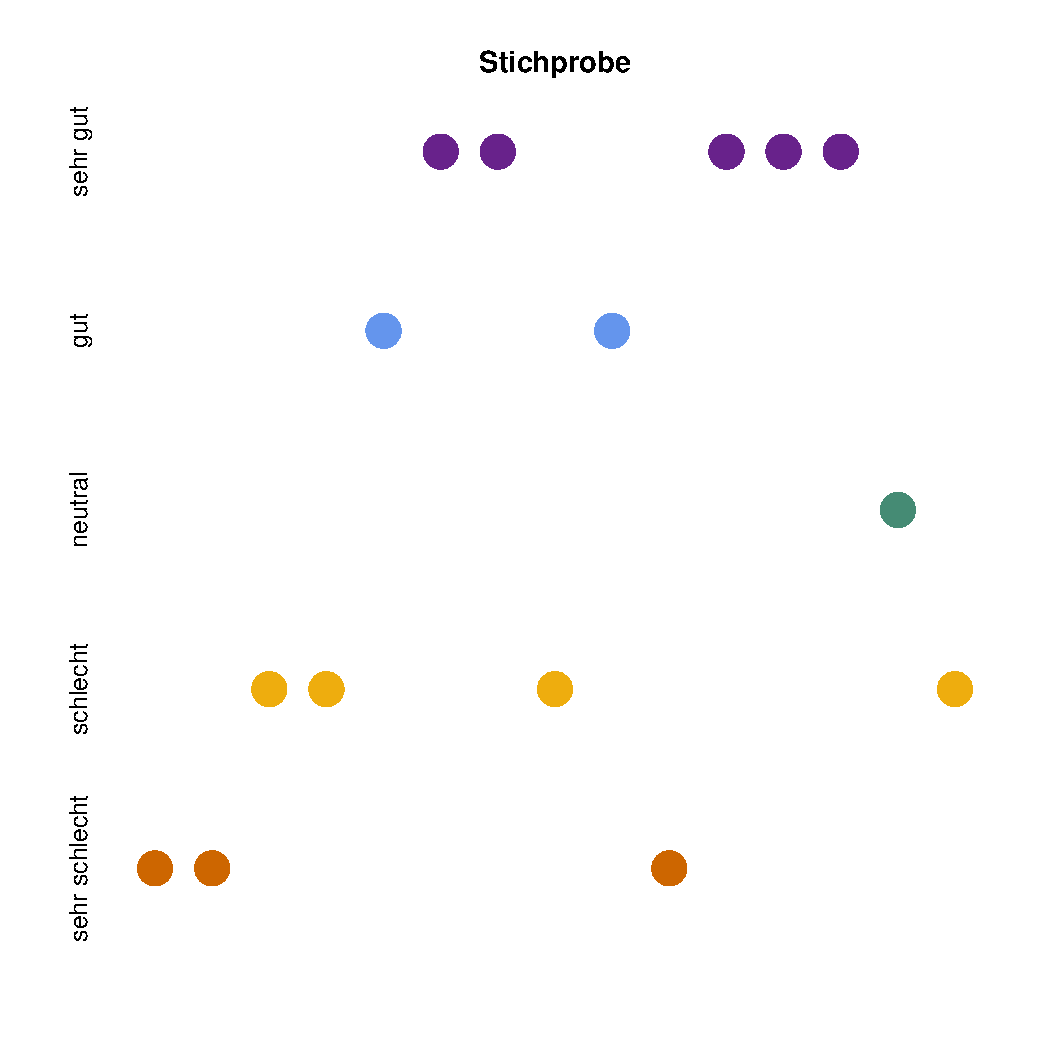
\includegraphics[height=0.9\textheight]{RVorlesung/median1a}
\end{frame}

\begin{frame}
  {Median bestimmen | Sortierte Stichprobe}
  \centering 
  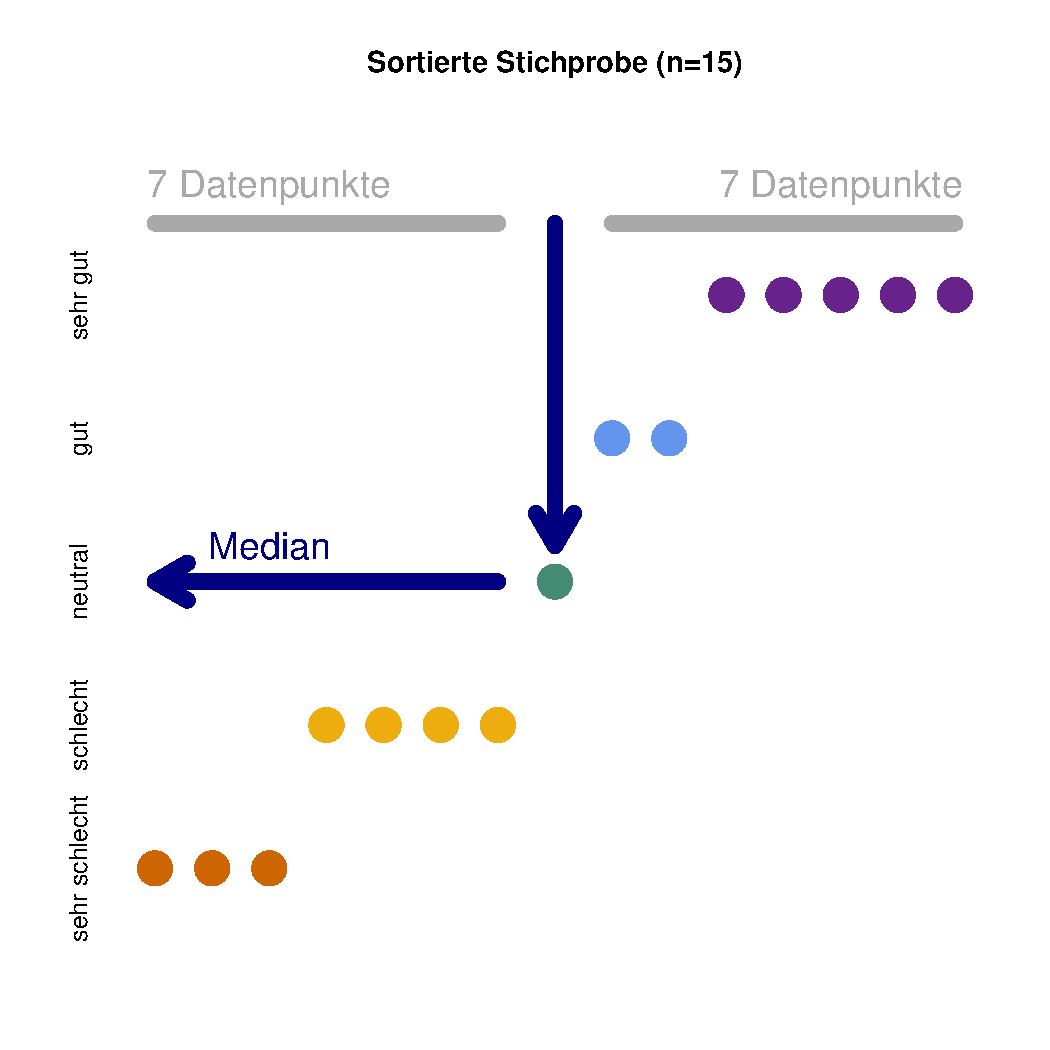
\includegraphics[height=0.9\textheight]{RVorlesung/median1b}
\end{frame}

\begin{frame}
  {Median bestimmen | Verzerrtere sortierte Stichprobe}
  \centering 
  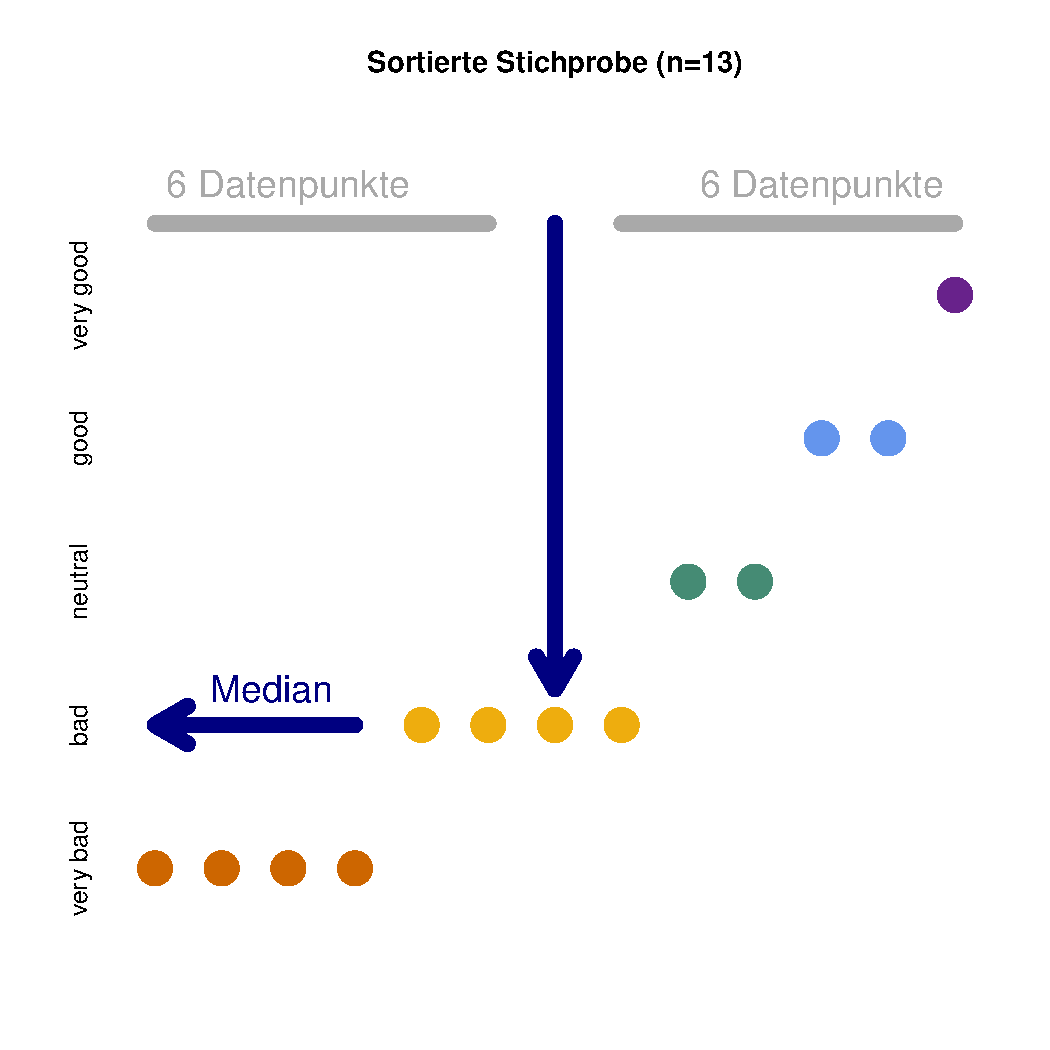
\includegraphics[height=0.9\textheight]{RVorlesung/median2}
\end{frame}

\begin{frame}
  {Zentraltendenz III}
  \alert{Arithmetisches Mittel} $\bar{x}$ | Summe aller Werte geteilt durch $n$ | \orongsch{ab Intervallskala}\\
  \Zeile
  \begin{multicols}{2}
    \centering 
    \hspace{0em}\\
    \vspace{0.1\textheight}
    $\bar{x}=\frac{\sum\limits_{i=1}^{n}x_i}{n}$
    \newpage
    \raggedright
    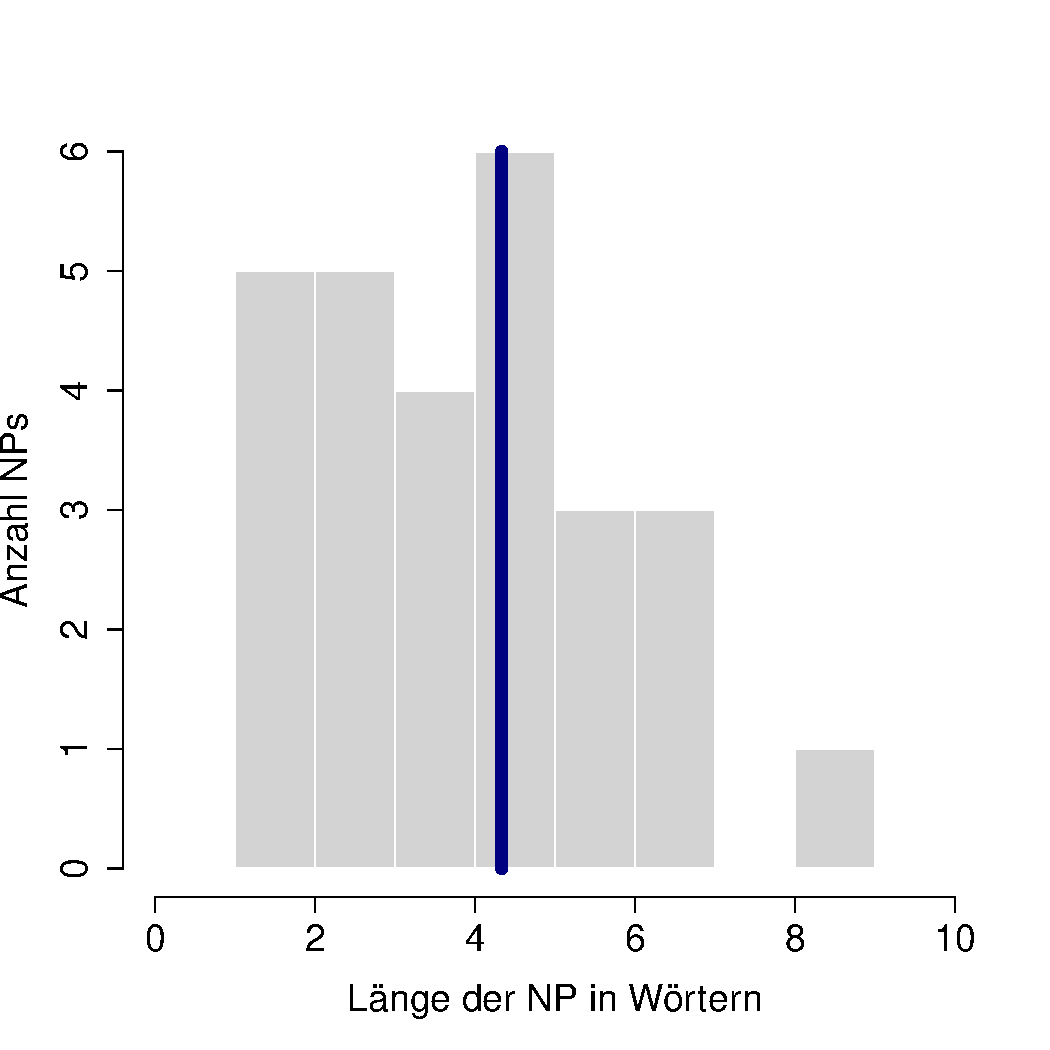
\includegraphics[height=0.6\textheight]{RVorlesung/mean}
  \end{multicols}
\end{frame}



\section{Empirische Verteilungen und Dispersion}

\begin{frame}
  {Warum sind Dispersionsmaße wichtig?}
  \alert{Dispersion} | Streuung der Daten\\
  \Zeile
  \begin{itemize}[<+->]
    \item \alert{Zentraltendenz} | Orientierung über Tendenzen der Stichprobe
     \Zeile 
    \item \alert{Ein Maß für Zentraltendenz} für \orongsch{beliebig viele Verteilungsformen}
      \Halbzeile
    \item Arithmetisches Mittel | deskriptiv oft \orongsch{unbrauchbar ohne Betrachtung der Verteilung}
    \item Median | \orongsch{auch nur bedingt besser}
  \end{itemize}
\end{frame}

\begin{frame}
  {Vier sortierte Stichproben}
  Jeder Punkt entspricht einem Datenpunkt\slash einer Messung!\\
  \begin{center}
    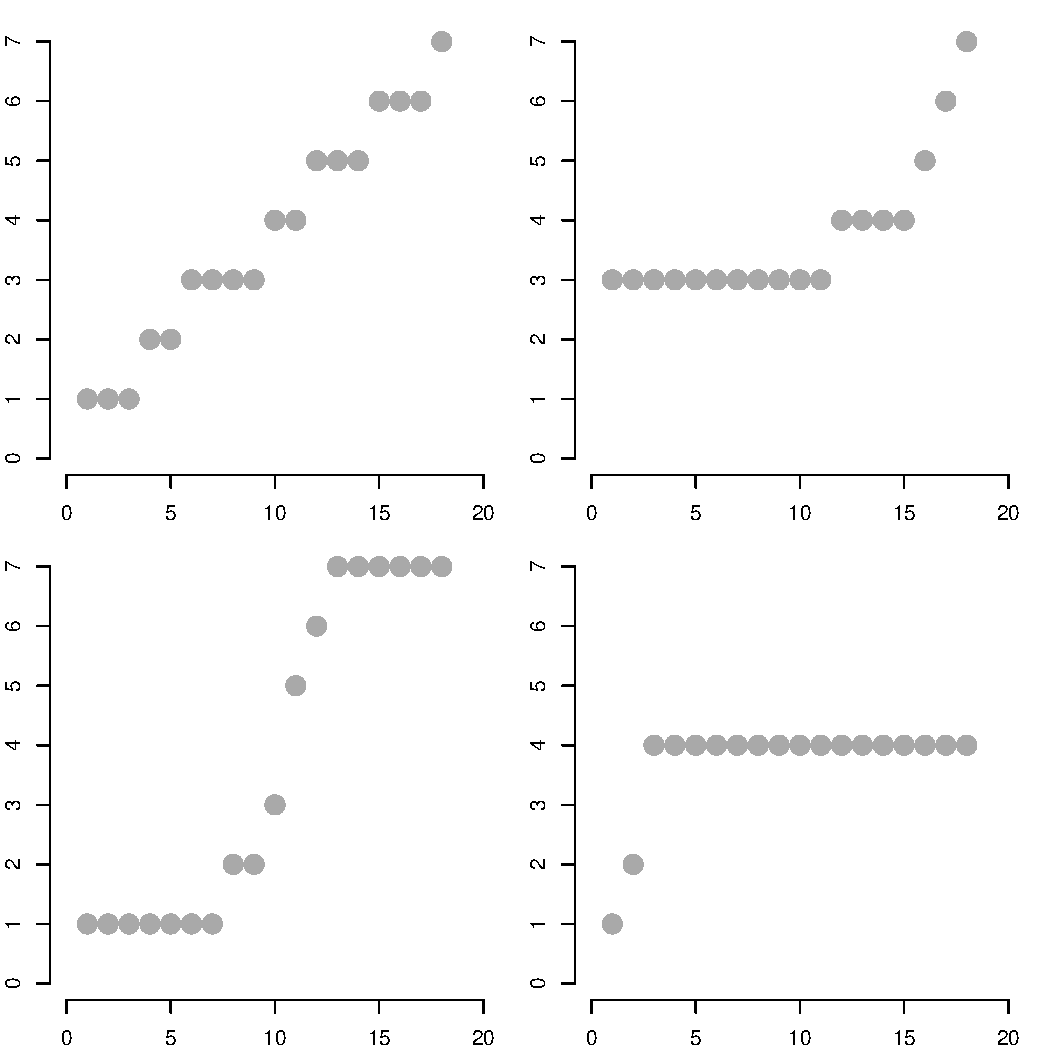
\includegraphics[height=0.75\textheight]{RVorlesung/foursamples}
  \end{center}
\end{frame}

\begin{frame}
  {Verteilungsformen}
  \alert{Histogramme} | Vier Stichproben mit \alert{$\bar{x}=3.72$} und \alert{$n=18$}\\
  \Viertelzeile
  \grau{Zum Beispiel 18 Bewertungen eines Probanden auf einer 7-Punkt-Skala}\\
  \begin{center}
    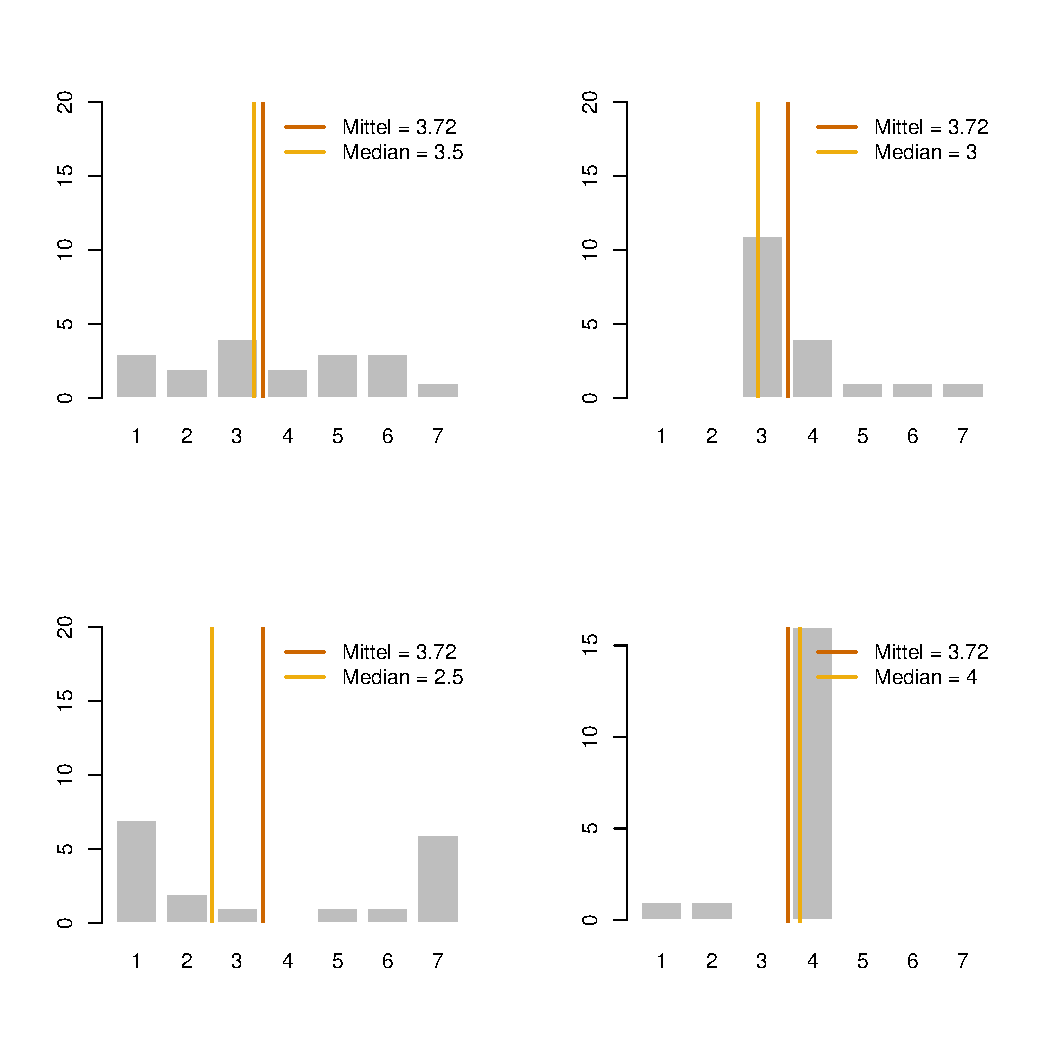
\includegraphics[height=0.75\textheight]{RVorlesung/fourdists}
  \end{center}
\end{frame}

\begin{frame}
  {Quartile}
  \alert{Quartile} | Generalisierung des Medians (bei 25 \%, 50 \%, 75 \%)\\
  \begin{center}
    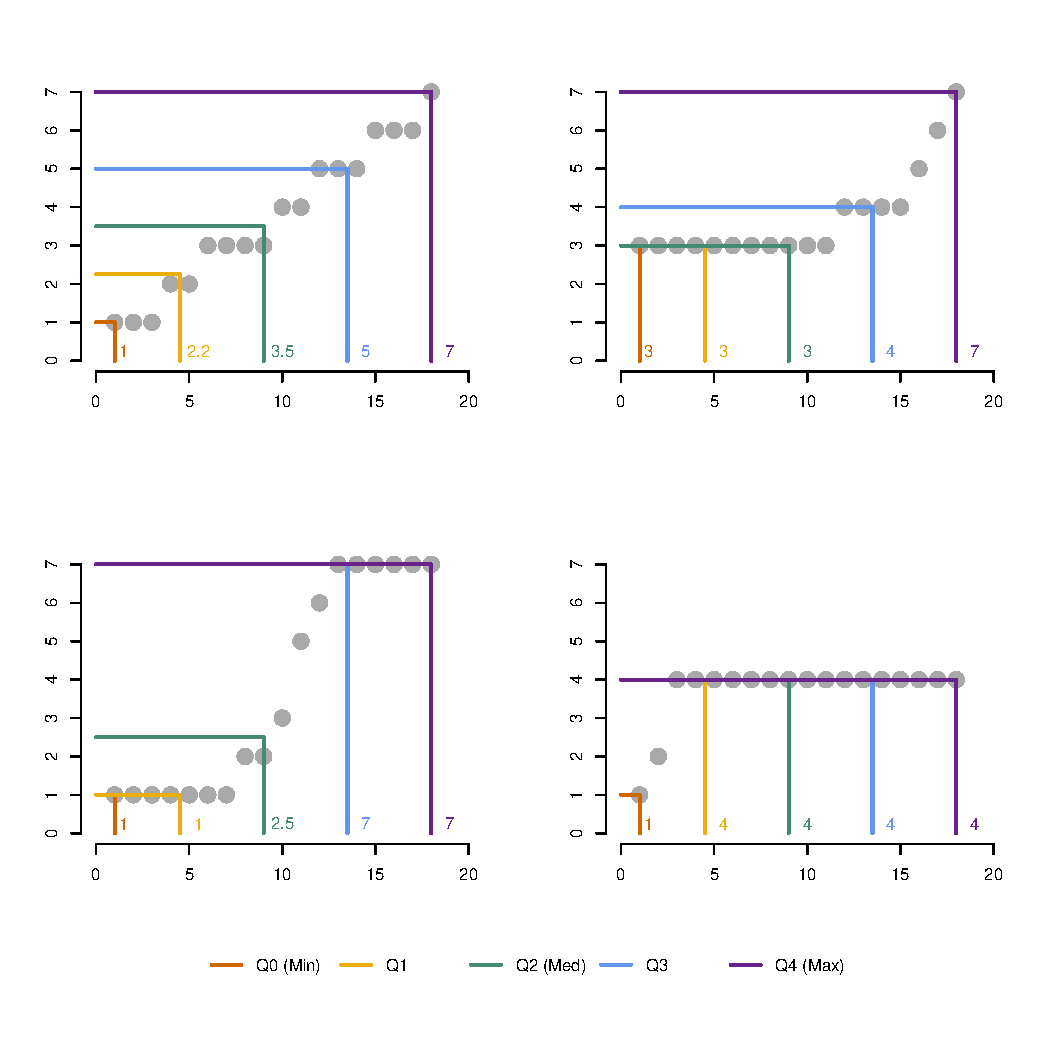
\includegraphics[height=0.85\textheight]{RVorlesung/fourquartiles}
  \end{center}
\end{frame}


\begin{frame}
  {Interquartilbereich, Boxplots und Violinplots}
  \begin{itemize}[<+->]
    \item Interquartilbereich \alert{$IQR = Q_3-Q_1$} | Die mittleren 50 \%
     \Zeile 
    \item Boxplots
      \Viertelzeile
      \begin{itemize}[<+->]
        \item \alert{Median} | Linie in der Mitte
        \item \alert{Oberes und unteres Quartil} | Boxen
        \item \alert{1,5-facher Interquartilabstand} | gestrichelte Hebel
        \item \alert{Ausreißer} | Punkte
      \end{itemize}
      \Halbzeile
    \item Violinplots | Zusätzlich Plot der Verteilungsdichte (statt Box)
  \end{itemize}
\end{frame}


\begin{frame}
  {Boxplots | Die bessere Zusammenfassung}
  \begin{center}
    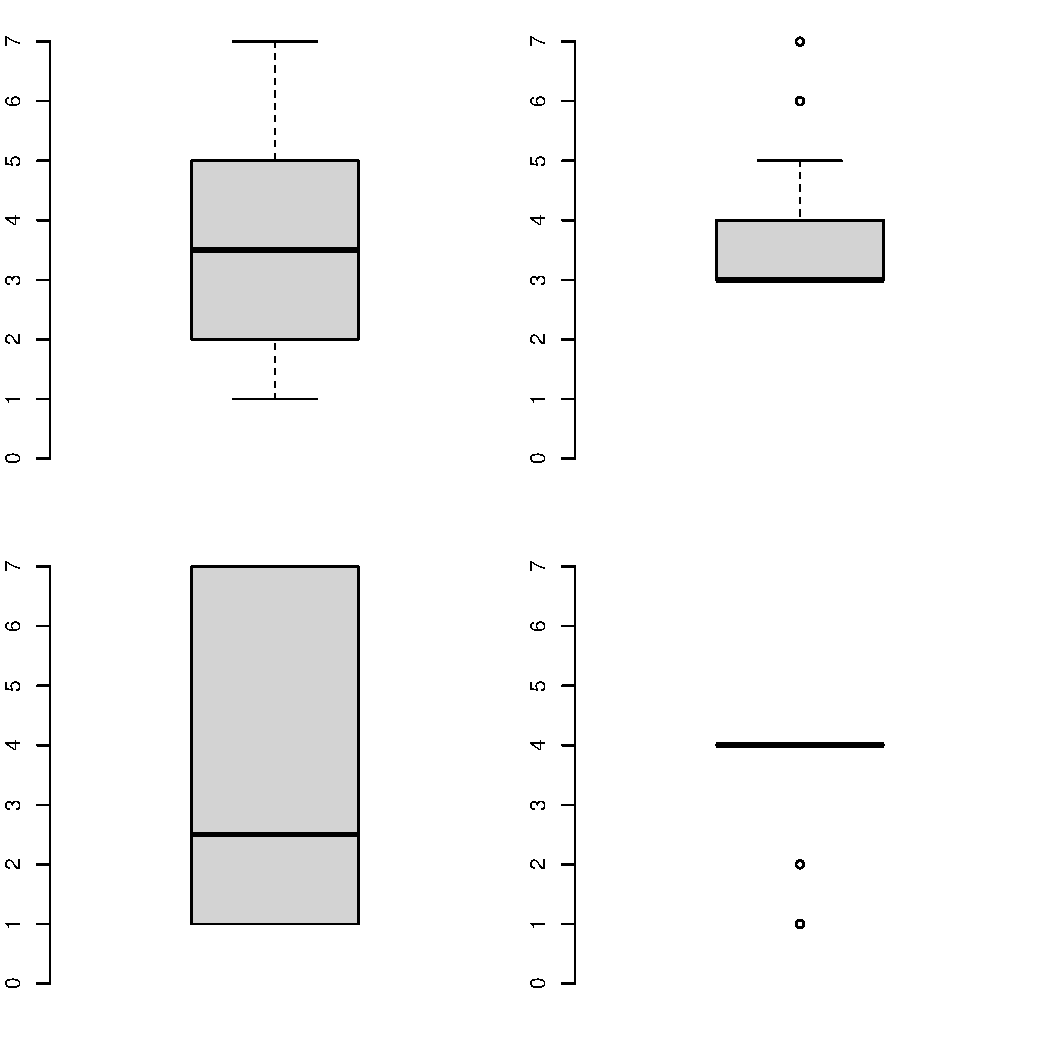
\includegraphics[height=0.7\textheight]{RVorlesung/fourbox}
  \end{center}
\end{frame}


\begin{frame}
  {Violinplots | Die noch bessere Zusammenfassung}
  \begin{center}
    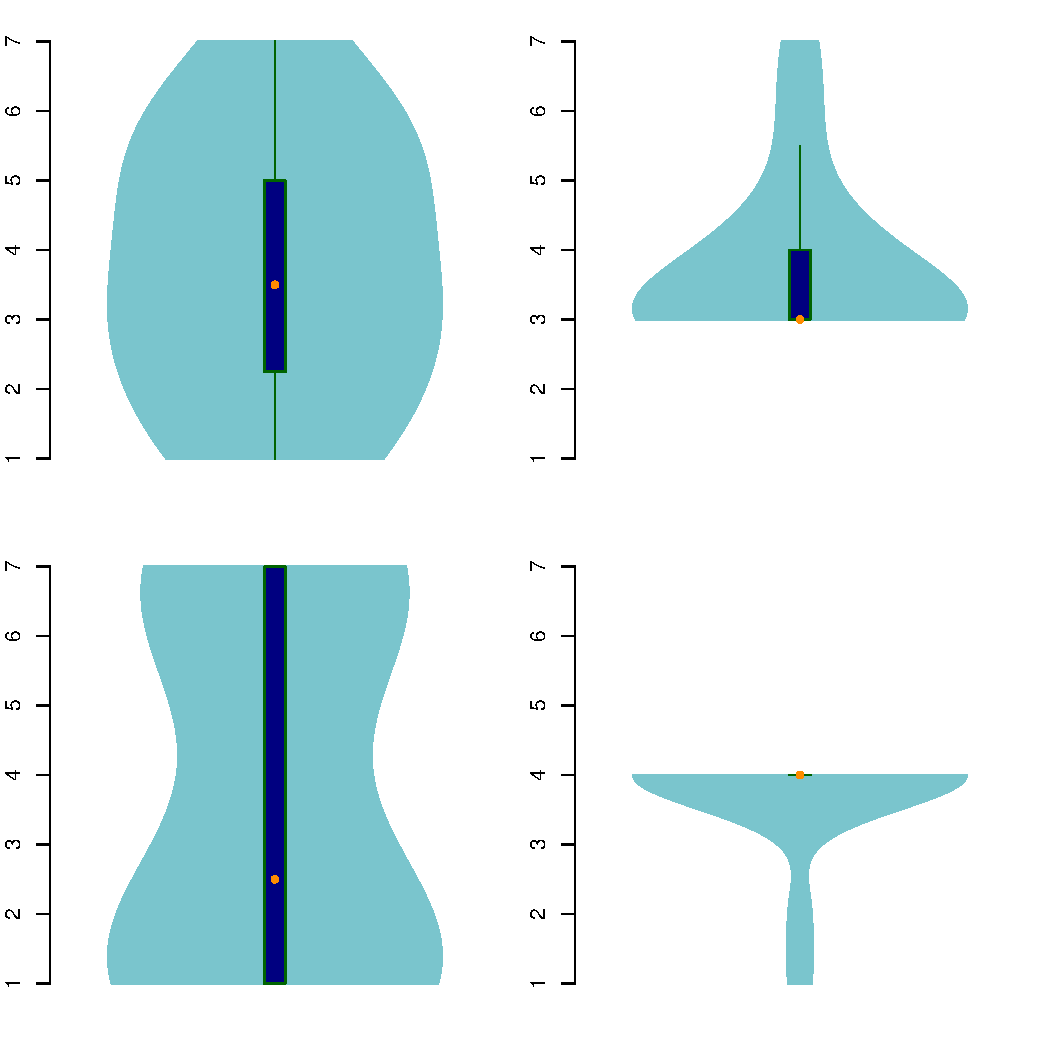
\includegraphics[height=0.7\textheight]{RVorlesung/fourviolins}
  \end{center}
\end{frame}

\begin{frame}
  {Was bestimmt die Varianz?}
  Die \alert{Distanzen der Messwerte zum Mittel} sind unterschiedlich groß.\\
  \begin{center}
    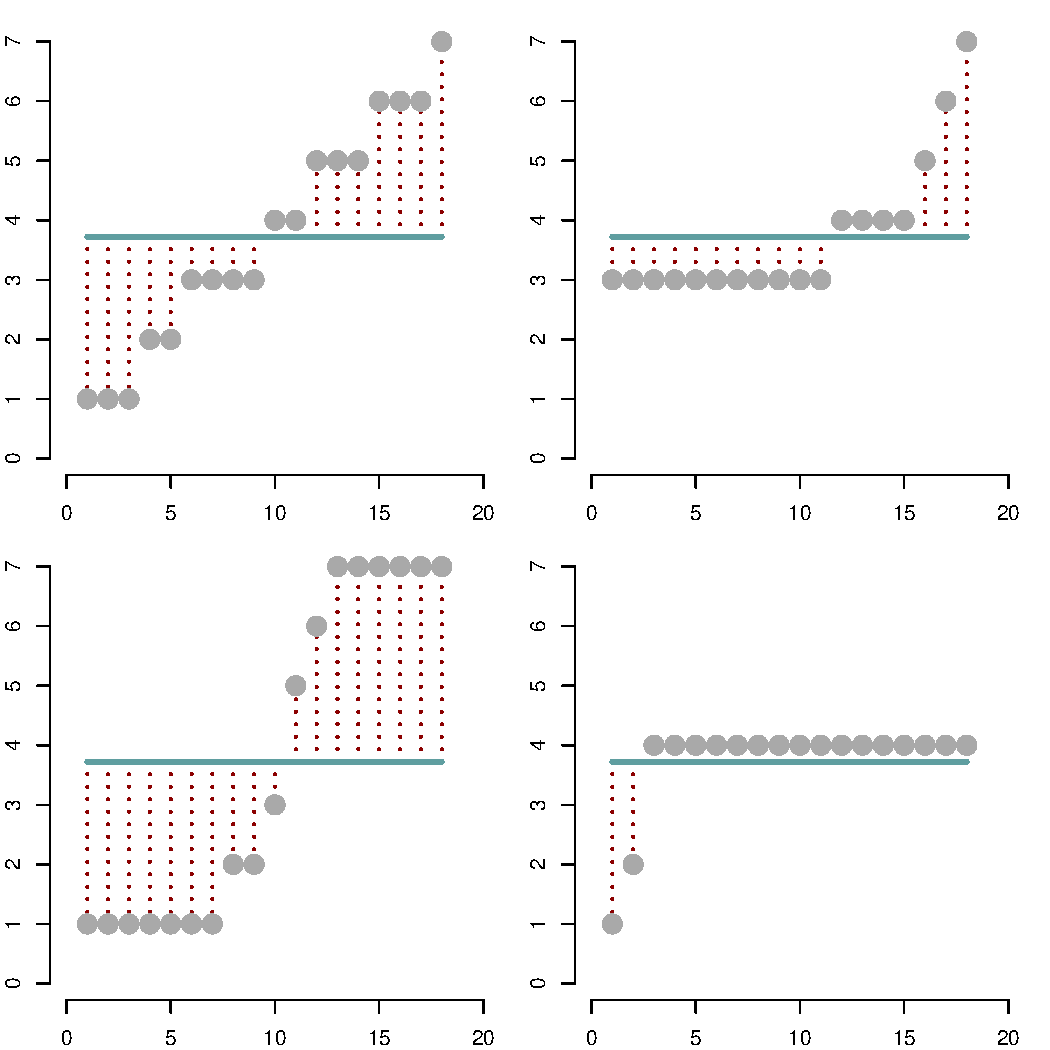
\includegraphics[height=0.7\textheight]{RVorlesung/fourvariances}
  \end{center}
\end{frame}


\begin{frame}
  {Varianz und Standardabweichung}
  \alert{Varianz $s^2$} | Quadrierte \alert{mittlere Abweichung} vom Mittelwert\\
      \begin{center}
	\alert{$s^2(x)=\frac{ \sum\limits_{i=1}^{n}(x_i-\bar{x})^2}{n-1}$}
      \end{center}
\pause
      \vspace{0.5cm}
    \alert{Standardabweichung $s$} | Quadratwurzel der Varianz\\
      \begin{center}
	\alert{$s(x)=\sqrt{s^2(x)}$}
      \end{center}
      \vspace{0.5cm}

  \pause
    \alert{Summe der Quadrate} | Zählerterm der Varianz\\
  \begin{center}
    $SQ(x)=\sum\limits_{i=1}^{n}(x_i-\bar{x})^2$
  \end{center}
\end{frame}

\begin{frame}
  {Unterschiedliche Standardabweichungen}
  \begin{center}
    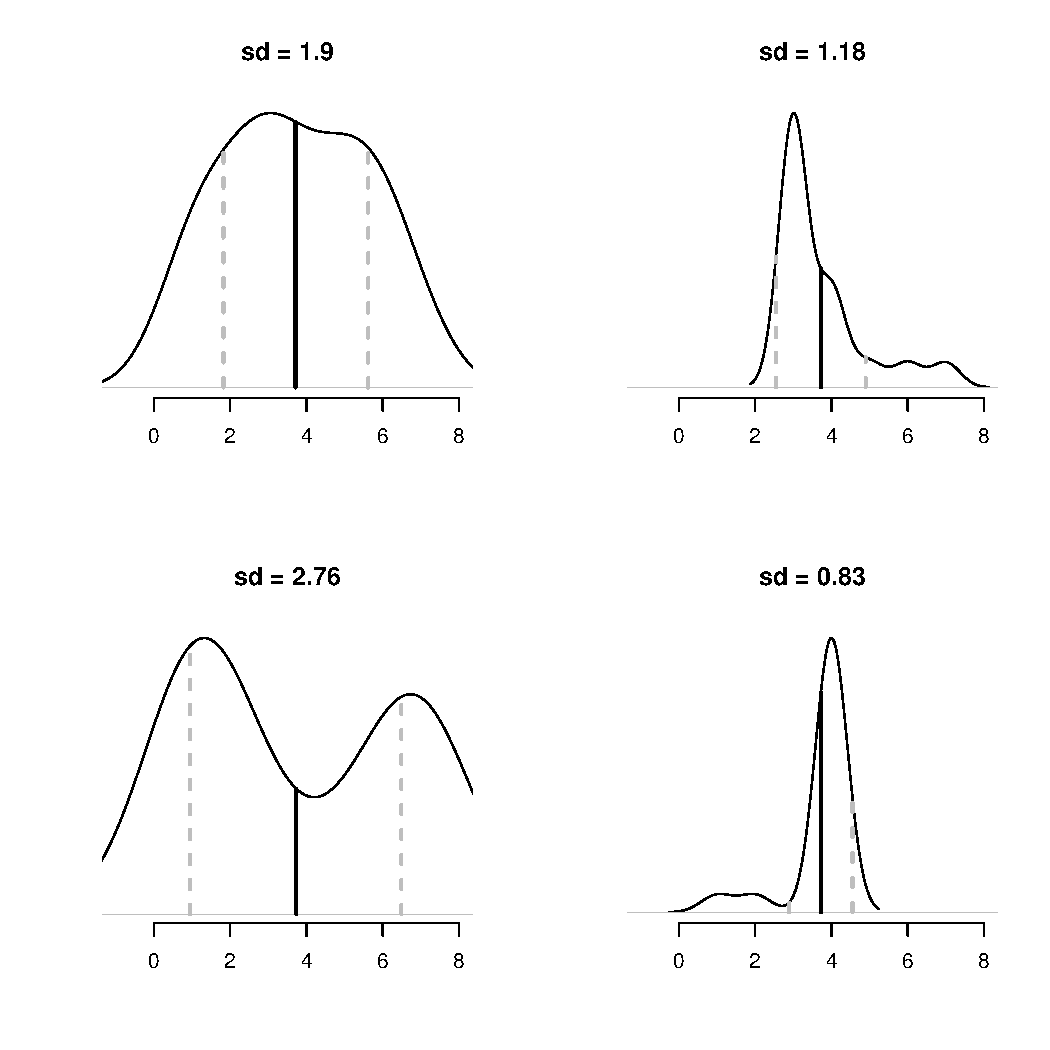
\includegraphics[height=0.9\textheight]{RVorlesung/stdevs}
  \end{center}
\end{frame}


\begin{frame}
  {z-Wert}
  Für jeden Messpunkt $x_i$ | \alert{$z_i=\frac{x_i-\bar{x}}{s(x)}$}\\
  \begin{center}
    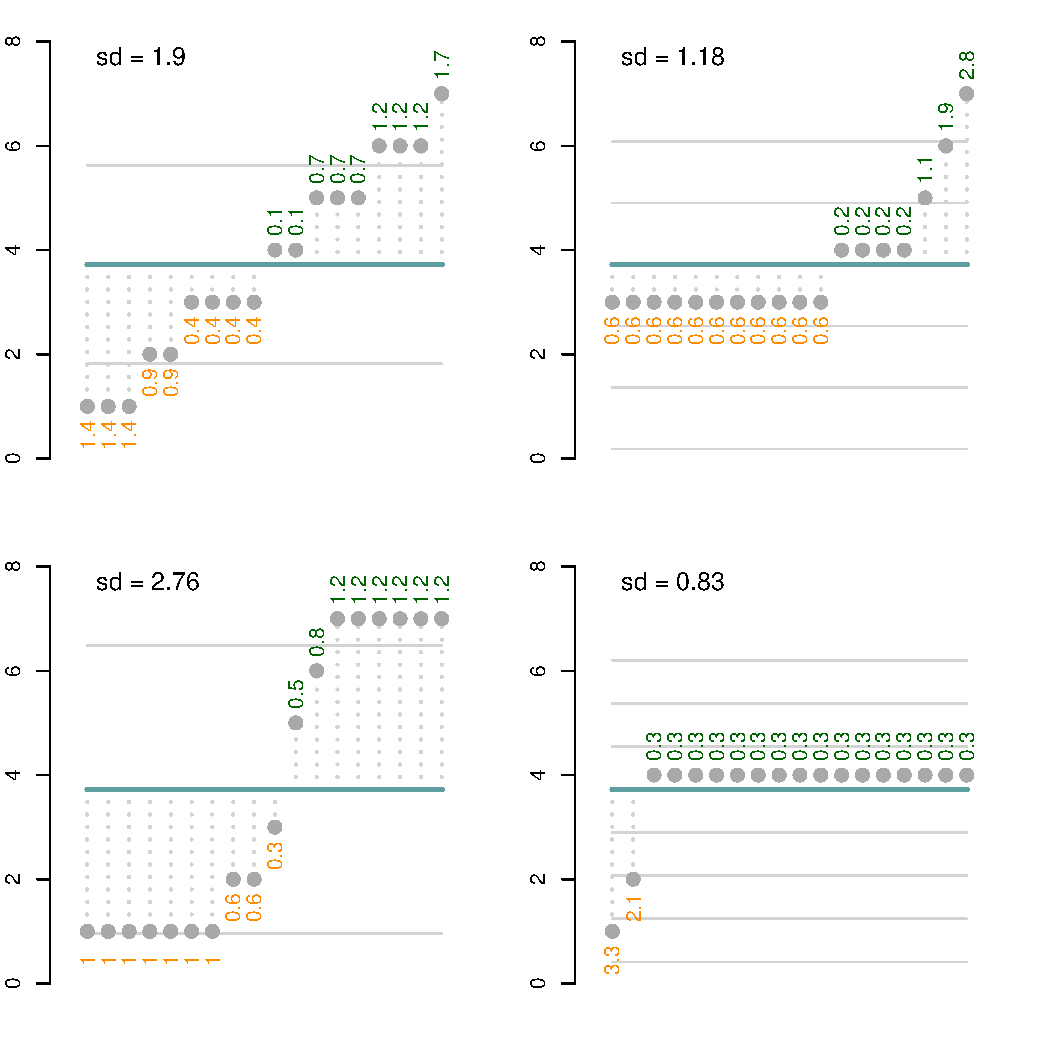
\includegraphics[height=0.8\textheight]{RVorlesung/fourzs}
  \end{center}
\end{frame}

\begin{frame}
  {z-Wert | Rechenbeispiel}
  \begin{itemize}[<+->]
    \item Bsp.: $\alert{x}=[3.9, 4.3, 7.2, 8.5, 11.1, 12.1, 14.0, 20.7]$
      \Halbzeile
      \begin{itemize}[<+->]
        \item $\alert{\bar{x}}=$\onslide<2->{$10.225$}
          \Halbzeile
        \item $\alert{s^2(x)}=$$\frac{(3.9-10.255)^2+\ldots+(20.7-10.225)^2}{8-1}=$$\frac{215.495}{7}=$$30.785$
          \Halbzeile
        \item $\alert{s(x)}=$$\sqrt{30.785}=$$5.548$
          \Halbzeile
        \item $\alert{z}=[\frac{3.9-10.225}{5.548}$, \ldots, $\frac{20.7-10.225}{5.548}]=$$[-1.140, -1.068, -0.545, -0.311, 0.158, 0.338, 0.680, 1.888]$
      \end{itemize}
  \end{itemize}
\end{frame}

\section{Bivariate Statistiken}

\begin{frame}
  {Zähldaten von zwei Variablen}
  \alert{Kreuztabelle} | Darstellung der Zähldaten zweier Variablen\\
  \Zeile
  \begin{center}
    \begin{tabular}{rcc}
      \cline{2-3}
      &&\\
      & \textbf{Variable 1 | Wert 1} & \textbf{Wert2} \\
      &&\\
      \hline
      &&\\
      \textbf{Variable 2 | Wert 1} & Anzahl $x_{11}$ & Anzahl $x_{12}$ \\
      &&\\
      \textbf{Wert 2} & Anzahl $x_{21}$ & Anzahl $x_{22}$ \\
      &&\\
      \hline
    \end{tabular}
  \end{center}
\end{frame}



\section{Standardfehler und Konfidenzintervalle}

\begin{frame}
  {Anteilswerte und Stichproben}
  \begin{itemize}[<+->]
    \item Das Verb \textit{essen} | Manchmal mit, manchmal ohne Akkusativ (direktes Objekt)
    \item Angenommenes wahres Verhältnis | \alert{Mit Objekt 39 \%, ohne Objekt 61 \%}
      \Halbzeile
    \item Viele Stichproben mit n=100 | Ergebnis \rot{nicht} immer 39 zu 61
     \Doppelzeile 
    \item \alert{95\%-Konfidenzintervall} \\
      \gruen{In welchem Bereich liegen 95\% aller Anteilswerte bei n=100?}
  \end{itemize}
\end{frame}


\begin{frame}
  {Sechzehn simulierte Stichprobenentnahmen (n=100)}
  \centering 
  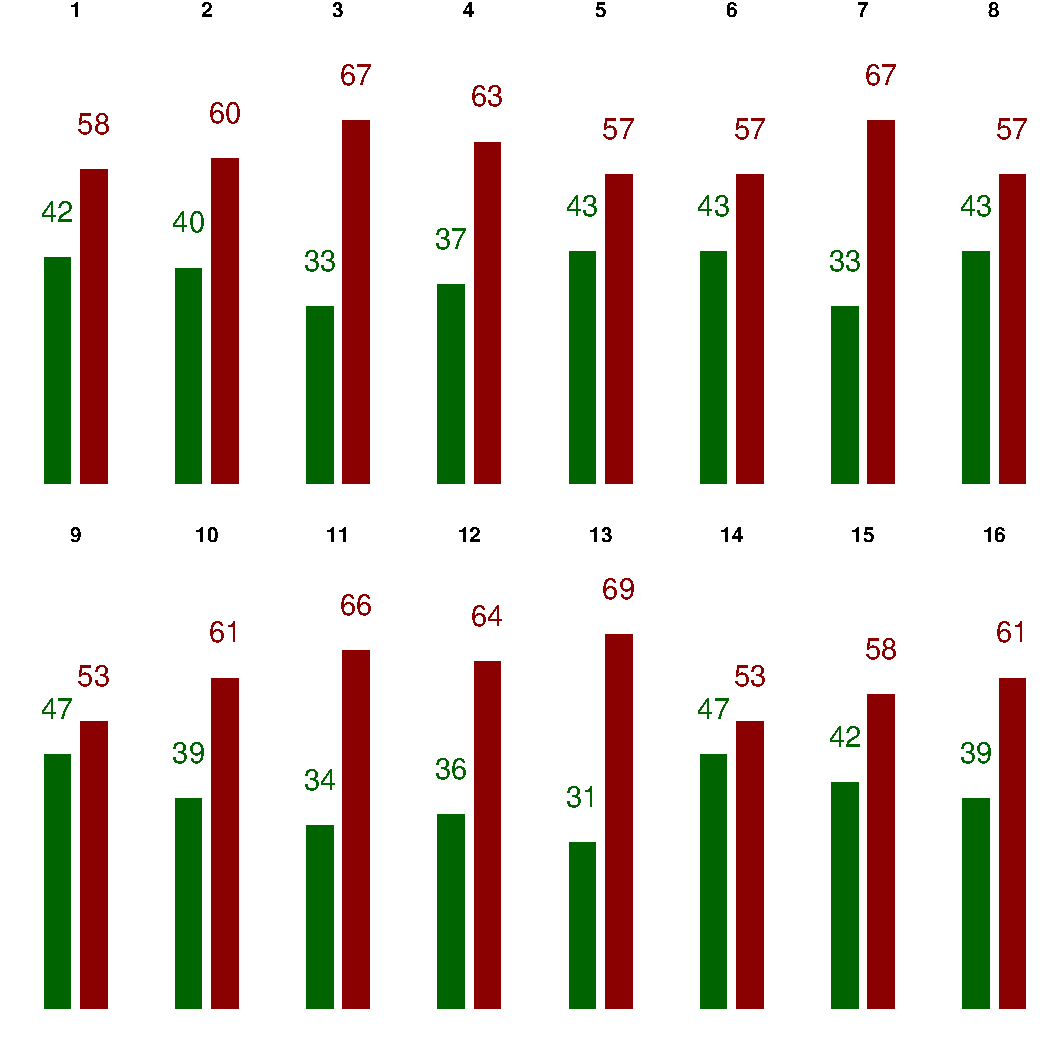
\includegraphics[height=0.8\textheight]{RVorlesung/sixteenbernoullis}
\end{frame}

\begin{frame}
  {Wiederholte Stichprobenentnahmen (n=100)}
  \centering 
  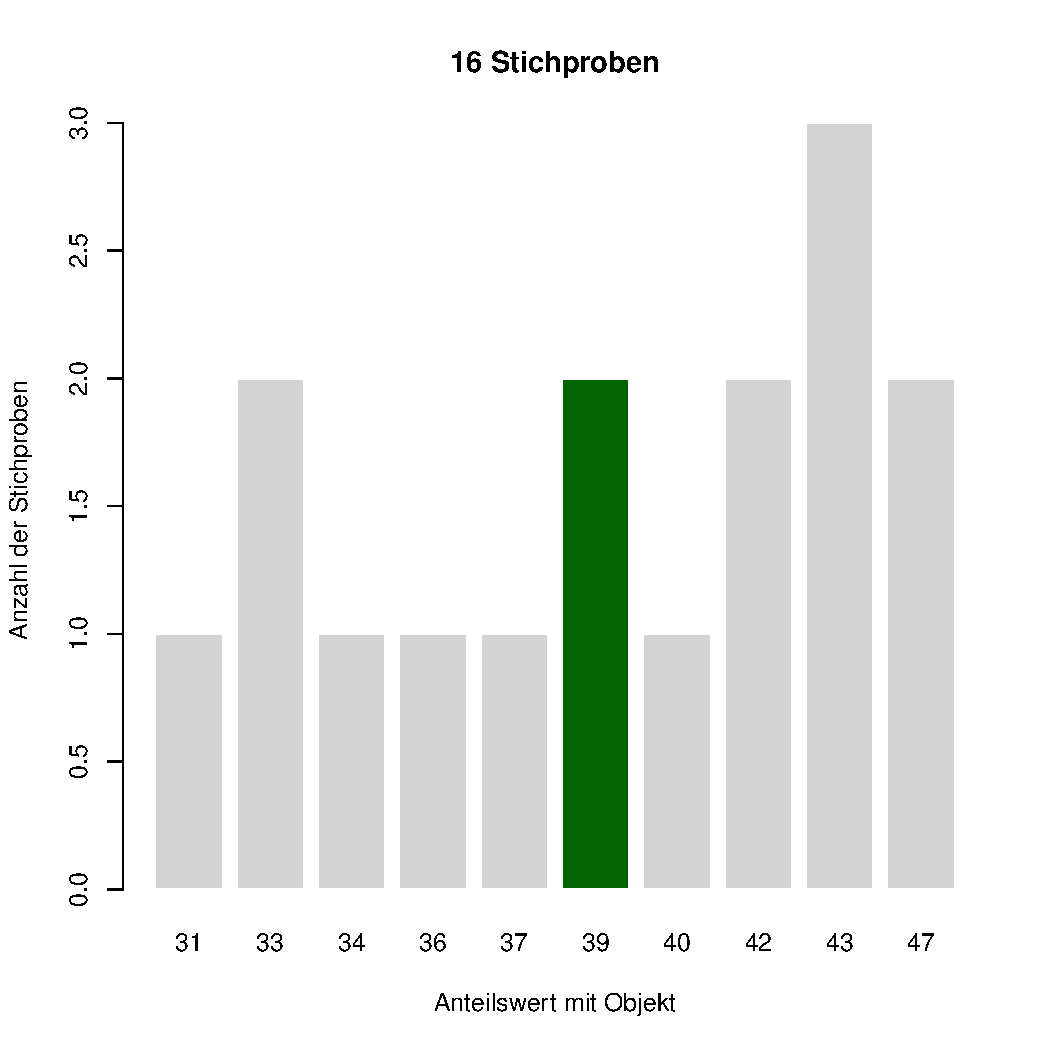
\includegraphics[width=0.3\textwidth]{RVorlesung/manybernoullis1}
  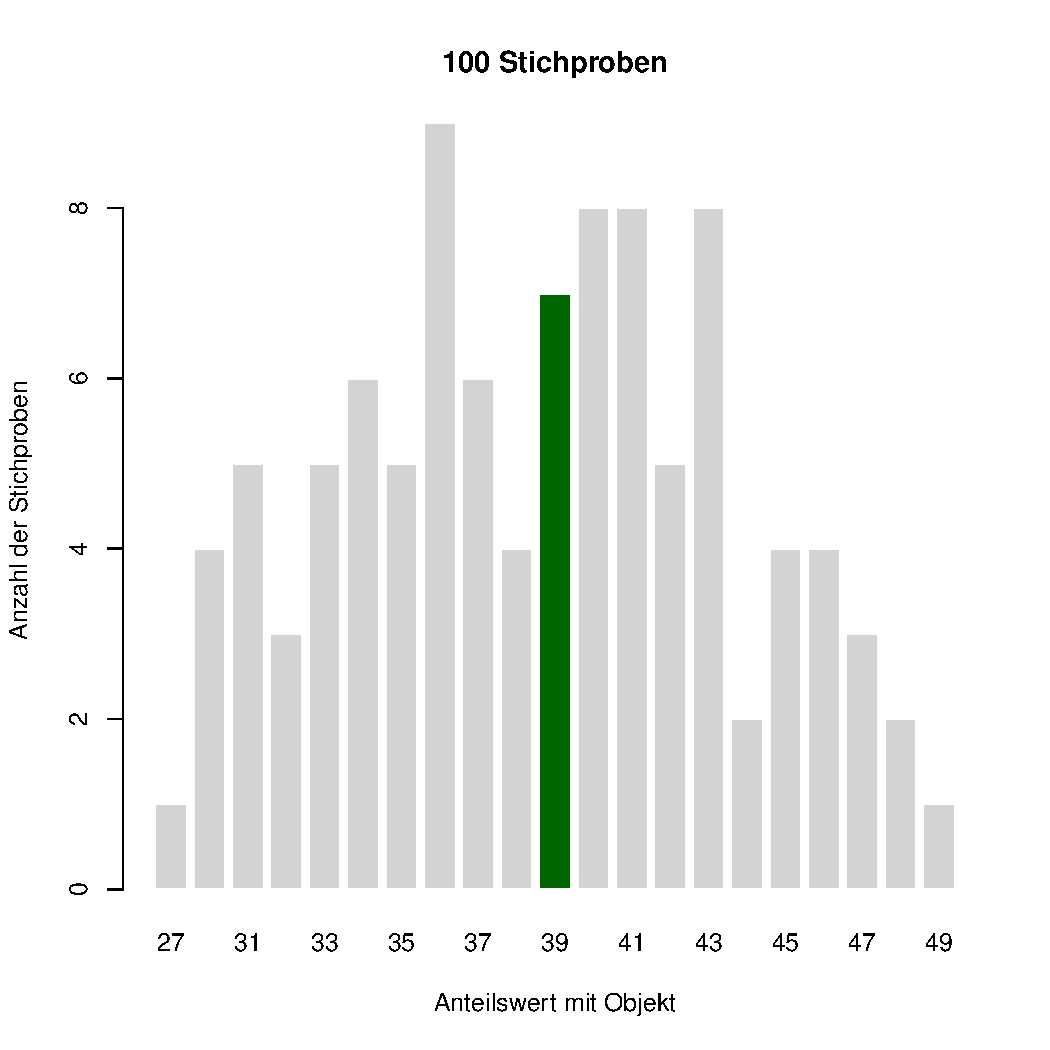
\includegraphics[width=0.3\textwidth]{RVorlesung/manybernoullis2}
  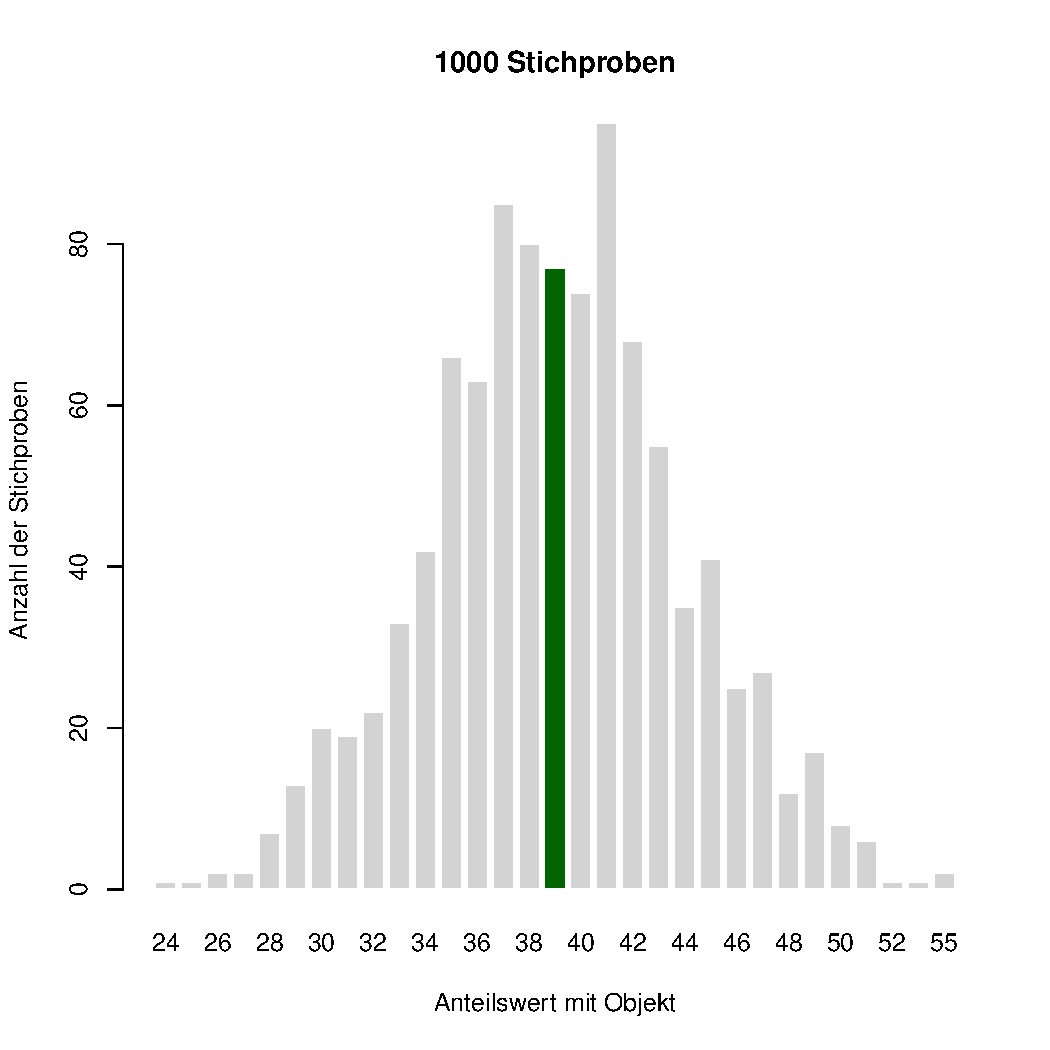
\includegraphics[width=0.3\textwidth]{RVorlesung/manybernoullis3}
\end{frame}


\begin{frame}
  {Standardfehler}
  \begin{itemize}[<+->]
    \item Die \alert{meisten $q$} | Nah am wahren Wert $Q$
    \item Sehr \alert{wenige $q$} | Weit von $Q$ entfernt
      \Halbzeile
    \item Bei unendlich vielen Messungen
      \begin{itemize}[<+->]
        \item \alert{\orongsch{Mittelwert} der gemessenen Anteilswerte gleich $Q$}
        \item Gemessene Anteilswerte \orongsch{normalverteilt um $Q$}
        \item \alert{Standardabweichung} der Messwerte um Q bekannt \ding{222} \gruen{Standardfehler}
      \end{itemize}
     \Zeile 
    \item \gruen{Standarfehler} | Standardabweichung der Messwerte
      \begin{itemize}[<+->]
        \item Bei \alert{gegebener Stichprobengröße $n$}
        \item Bei einem \alert{bekannten Populationsanteil Q}
      \end{itemize}
  \end{itemize}
\end{frame}

\begin{frame}
  {Standardfehler für Anteilswerte | Berechnung}
  \begin{itemize}[<+->]
    \item Für einen wahren Anteilswert $Q$
    \item Bei Stichprobengröße $n$
  \end{itemize}
  \Halbzeile
  \begin{center}
    \alert{$SF(Q,n)=\sqrt{\frac{Q\cdot(1-Q)}{n}}$}\\
    \Doppelzeile
    Bsp. für $Q=0.39$ und $n=100$ | $SF(q)=\sqrt{\frac{0.39\cdot(1-0.39)}{100}}=0.0488$
  \end{center}
\end{frame}

\begin{frame}
  {Standardfehler | Interpretation}
  \begin{center}
    \alert{$SF(Q,n)=\sqrt{\frac{Q\cdot(1-Q)}{n}}$}\\

    \vspace{.1cm}
    Bsp.: $SF(0.39,100)=\sqrt{\frac{0.39\cdot(1-0.39)}{100}}=0.0488$
  \end{center}
  \Zeile
  \begin{itemize}[<+->]
    \item Für \alert{beliebig viele} Stichproben
    \item Bei \alert{Stichprobengröße $n=100$}
    \item Aus einer Grundgesamtheit mit \alert{wahrem Anteilswert $Q=0.39$}
      \Halbzeile
    \item Abweichung der gemessenen Anteile von $Q=0.39$ mit einem \alert{$SF=0.0488$}
  \end{itemize}
\end{frame}


\begin{frame}
  {Konfidenzintervall | Standardfehler und Normalverteilung}
  \alert{Normal-\slash Gaussverteilung} | Parameter \alert{Mittelwert} und \alert{Standardabweichung}\\
  \Viertelzeile
  \ding{222} Mathematisch exhaustiv bekannt, Flächen unter der Kurve usw.\ berechenbar\\
  \centering
  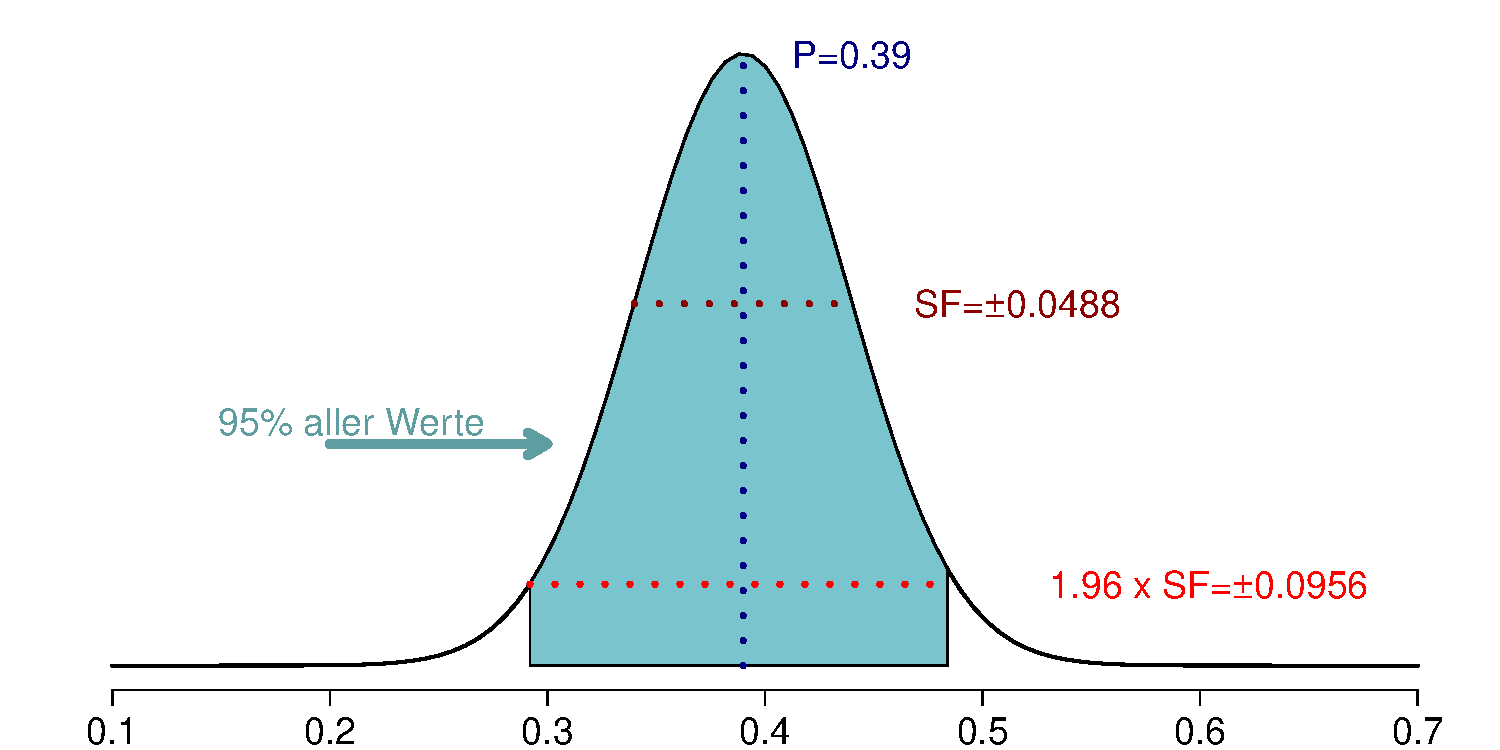
\includegraphics[height=0.75\textheight]{RVorlesung/ci95}
\end{frame}


\begin{frame}
  {Verteilungsfunktion der Normalverteilung}
  \onslide<+->
  \onslide<+->
  \centering 
  \LARGE
  \begin{math}
    p(\orongsch{x})=\grau{\frac{1}{\gruen{\sigma}\sqrt{2\pi}}}e^{-\frac{1}{2}\left(\frac{\orongsch{x}-\alert{\mu}}{\gruen{\sigma}}\right)^2}
  \end{math}\\
  \large
  \Doppelzeile
  Wenn Sie mehr wissen möchten:\\
  \url{https://youtu.be/cy8r7WSuT1I}\\
  Großartiges Video von Grant Sanderson (3blue1brown)
\end{frame}


\begin{frame}
  {Konfidenzintervall | z-Werte}
  \begin{itemize}[<+->]
    \item Stichproben (wie erwähnt) \alert{normalverteilt} 
    \item Der \alert{z-Wert}, zum Beispiel für $\alpha=0.95$: \alert{$z(0.95)$} beantwortet:\\
      \orongsch{Wie viele Standardfehler definieren 95\% der Fläche unter der Kurve?}
      \Zeile
    \item \alert{Quantilfunktion der Normalverteilung} | In R mit \alert{\texttt{qnorm()}} oder \alert{Tabelle}
    \item Quantilfunktion | Wie viele Standardabweichungen trennen auf jeder Seite 2.5\% ab?
    \item \alert{\texttt{qnorm(0.025, lower.tail=FALSE)}} \ding{222} \orongsch{$z(0.95) = 1.96$}
  \end{itemize}
\end{frame}

\begin{frame}
  {Konfidenzintervall | Standardfehler um wahren Anteilswert}
  \begin{itemize}[<+->]
    \item Standardfehler | \alert{Standardabweichung} der Stichprobenwerte
    \item \alert{Konfidenzbreite} | \orongsch{z-Wert multipliziert mit Standardfehler}
    \item 95\% der Werte | Intervall \orongsch{Anteilswert ± Konfidenzbreite}
  \end{itemize}
  \Doppelzeile
  \begin{center}
    \alert{$KI(Q,n,\alpha)=Q\pm z(\alpha)\cdot SF(Q,n)$}\\
    \Zeile
  Bsp.: $KI(0.39,100,0.95)=0.39\pm1.96\cdot 0.0488=0.39\pm0.096=\alert{[0.29, 0.49]}$
  \end{center}
\end{frame}

\begin{frame}
  {Interpretation}
  \begin{center}
    Konfidenzintervall im Beispiel | \alert{0.29 bis 0.49}\\
    \Halbzeile
    In 95\% aller Stichproben mit $n=100$ liegt der Messwert\\
    zwischen $0.29$ und $0.49$ bei einem wahren Anteil von 0.39.
  \end{center}
  \Zeile
  \begin{itemize}[<+->]
    \item Praxis | \orongsch{Wahrer Anteil nicht bekannt}, daher \orongsch{Schätzung aus Stichprobenanteil $q$}
    \Zeile
    \item \rot{Der gemessene Anteil $q$ kann aber eine totale Fehlschätzung sein!}
    \item Die Philosophie dahinter geht von \alert{wiederholten Messungen} aus.
      \Halbzeile
    \item Entweder liegt der gemessene Wert im Konfidenzintervall,\\
      \rot{oder ein seltenes Ereignis ist eingetreten}.
      \Halbzeile
    \item \rot{\textbf{Falsche Interpretation}:\\Wir sind zu 95\% sicher, dass der wahre Wert zwischen 0.29 und 0.49 liegt.}
  \end{itemize}
\end{frame}

\begin{frame}
  {Konfidenzintervall | Breite bei verschiedenen Q, n und $\alpha$}
  \centering 
  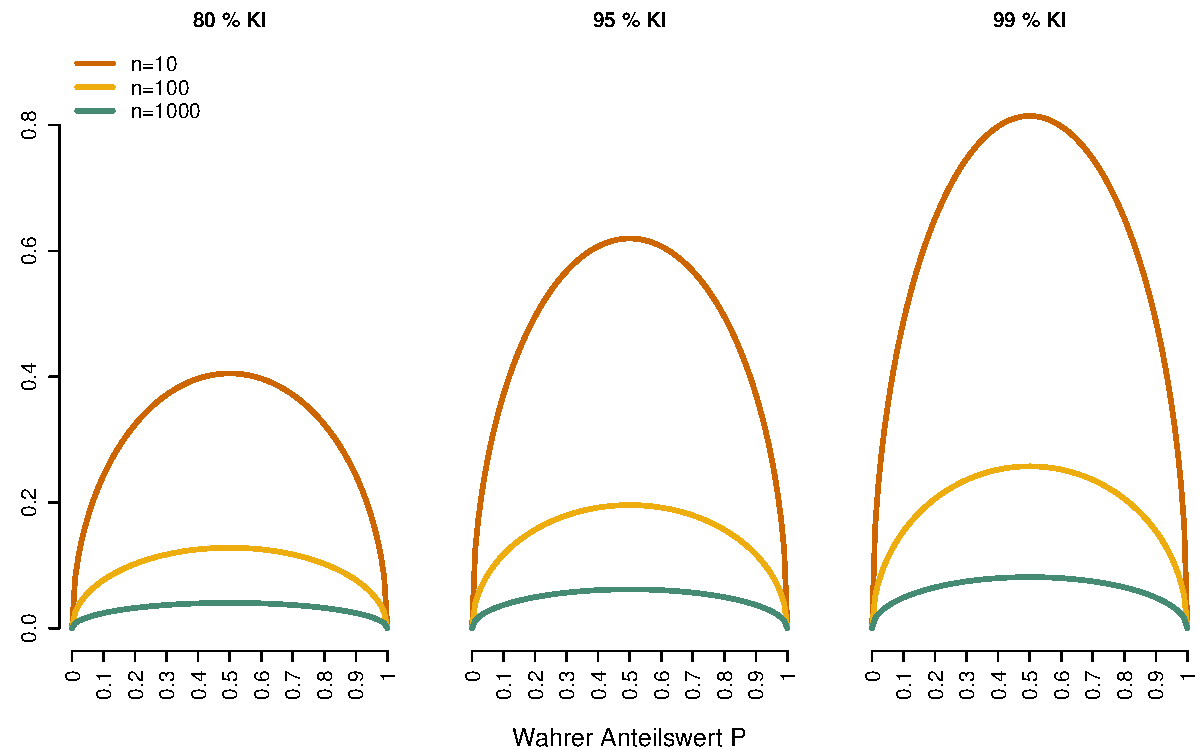
\includegraphics[height=0.85\textheight]{RVorlesung/threecis}
\end{frame}

\begin{frame}
  {Konfidenzintervall für Mittelwerte}
  \onslide<+->
  \onslide<+->
  Parallel zum KI für Anteilswerte: \alert{KI für Mittelwerte} mit \orongsch{derselben Formel}\\
  \Doppelzeile
  \onslide<+->
  \centering 
  Nur der Standardfehler wird anders berechnet:\\
  \Zeile
  \alert{$SF(\sigma, n)=\frac{\sigma}{\sqrt(n)}$}\\
  \Halbzeile
  \grau{$KI(\bar{x},n,\alpha)=\bar{x}\pm z(\alpha)\cdot SF(\sigma,n)$}\\
  \onslide<+->
  \Doppelzeile
  Interpretation des KI (95\%): Für einen \alert{beliebigen Mittelwert $\bar{x}$}\\
  und die \alert{wahre Standardabweichung der Population $\sigma$} liegen\\
  im Grenzwert exakt \alert{95\% aller Stichproben der Größe $n$ im 95\%-KI}.\\
  \Zeile
  Hier wird die wahre Standardabweichung $\sigma$ ggf.\\
  aus der Standardabweichung $s(x)$ Stichprobe geschätzt.
\end{frame}

\begin{frame}
  {Zur Interpretation des KIs}
  \onslide<+->
  \onslide<+->
  \centering 
  Schauen Sie sich möglichst mein (sehr altes) Video zur Interpretation von KIs an,\\
  auch wenn ich deutlich weniger im Kopf habe als Grant Sanderson.\\
  \Zeile
  \url{https://www.youtube.com/watch?v=TG8Z3RXL4E8X}
\end{frame}


\begin{frame}
  {Kritische Werte für Normalverteilung}
  \centering 
  \begin{tabular}[h]{ccp{0.1\textwidth}cc}
    \toprule
    \textbf{$\alpha$} & \textbf{$z(\alpha)$} && \textbf{$\alpha$} & \textbf{$z(\alpha)$}\\
    \midrule
    0.99 & 2.576 && 0.84 &  1.405 \\
    0.98 & 2.326 && 0.83 &  1.372 \\
    0.97 & 2.170 && 0.82 &  1.341 \\
    0.96 & 2.054 && 0.81 &  1.311 \\
    0.95 & 1.960 && 0.80 &  1.282 \\
    0.94 & 1.881 && 0.79 &  1.254 \\
    0.93 & 1.812 && 0.78 &  1.227 \\
    0.92 & 1.751 && 0.77 &  1.200 \\
    0.91 & 1.695 && 0.76 &  1.175 \\
    0.90 & 1.645 && 0.75 &  1.150 \\
    0.89 & 1.598 && & \\ 
    0.88 & 1.555 && & \\ 
    0.87 & 1.514 && & \\ 
    0.86 & 1.476 && & \\ 
    0.85 & 1.440 && & \\ 
    \bottomrule
  \end{tabular}
\end{frame}

\ifdefined\TITLE
  \section{Nächste Woche | Überblick}

  \begin{frame}
    {Einzelthemen}
    \begin{enumerate}
      \item Inferenz
      \item Deskriptive Statistik
      \item \alert{Nichtparametrische Verfahren}
      \item z-Test und t-Test
      \item ANOVA
      \item Freiheitsgrade und Effektstärken
      \item Power und Severity
      \item Lineare Modelle
      \item Generalisierte Lineare Modelle
      \item Gemischte Modelle
    \end{enumerate}
  \end{frame}
\fi

  \let\subsection\section\let\section\woopsi

  \section{z-Test und t-Test}
  \let\woopsi\section\let\section\subsection\let\subsection\subsubsection
  
\section{Übersicht}

\begin{frame}
  {Übersicht}
  \begin{itemize}[<+->]
%    \item Intuitive Einführung in das Konzept der Freiheitsgrade.
    \item Wann sind Unterschiede zwischen Mittelwerten signifikant?
    \item Mittelwerte in Grundgesamtheiten und Stichproben
  \end{itemize}
\end{frame}

\begin{frame}
  {Literatur}
  \begin{itemize}
    \item \citet{GravetterWallnau2007}
    \item \citet{Bortz2010}
      \vspace{\baselineskip}
    \item oder eben gleich \citet{Fisher1935a}
  \end{itemize}
\end{frame}


\section{Wiederholungen}


\subsection{Logik von statistischen Tests}

\begin{frame}
  {Tests in Fishers Philosophie}
  \begin{enumerate}
    \item \alert{Nullhypothese} (\Null) festlegen: Der theoretisch angenommene Effekt\\
      existiert \alert{nicht} (z.\,B.: Die Versuchsperson [VP] kann \alert{nicht} erkennen,\\
      ob Tee oder Milch zuerst in der Tasse war).
    \item \alert{Stichprobengröße} und \alert{Versuchsaufbau} festlegen (z.\,B.\ acht Tassen\\
      mit vier \textit{Tee zuerst}-Tassen; VP kennt das Verhältnis)
    \item \alert{\Sig-Niveau} festlegen: Wie unwahrscheinlich darf das Ergebnis\\
      unter Annahme der \Null\ sein, damit wir die \Null\ zurückweisen.
    \item Experiment durchführen, Ergebnis messen.
    \item \alert{p-Wert} berechnen: Wie wahrscheinlich \alert{war} es, dieses Ergebnis\\
      oder ein extremeres Ergebnis zu erreichen, wenn die \Null\ die Welt korrekt beschreibt.
    \item Wenn \alert{$p\leq$\,\Sig}, dann \Null\ zurückweisen: Entweder der Effekt existiert\\
      (\zB die VP kann die Reihenfolge des Einschenkens erkennen)\\
      \alert{oder ein seltenes Ereignis ist eingetreten}.
  \end{enumerate}
\end{frame}

\begin{frame}
  {Einschränkungen und Probleme bei der Interpretation}
  \begin{itemize}
    \item Voraussetzung: \alert{echte Zufallsstichprobe}
    \item Ergebnis: \alert{kein Beweis}
    \item keine Auskunft darüber, wie "`wahrscheinlich"' der Effekt ist
    \item keine Auskunft darüber, wie stark wir von der Existenz des Effekts\\
      überzeugt sein sollten (= \textit{inverse probability})
    \item jede \Null-Zurückweisung: nur ein kleinteiliger Hinweis auf einen Effekt
    \item \alert{substantielle} theoretische Hypothese oft und hart testen!
      \vspace{\baselineskip}
    \item \alert{Sensitivity}: keine Auskunft über die \alert{Stärke} des Effekts
      \begin{itemize}
        \item große Stichprobe $\rightarrow$ hohe Sensitivität
        \item kleine Strichprobe $\rightarrow$ niedrige Sensitivität
        \item je sensitiver desto leichter werden schwache Effekte signifikant
        \item Abhilfe bei Neyman-Pearson: \alert{Power} (Teststärke) vor dem Experiment
        \item quasi-kompatibel zu Fisher: \alert{Effektstärke} nach dem Experiment
      \end{itemize}
  \end{itemize}
\end{frame}

\begin{frame}
  {Und beim Konfidenzintervall?}
  Am Beispiel des 95\%-Konfidenzintervalls (KI)
  \begin{itemize}
    \item \rot{Falsch}: Wir können zu 95\% sicher sein, dass der wahre Wert im KI liegt.
    \item \rot{Falsch}: Der wahre Wert liegt mit 95\% Wahrscheinlichkeit im KI.
      \vspace{\baselineskip}
    \item Warum? \alert{Wenn der wahre Wert nicht im geschätzten KI liegt,\\
      ist die Wahrscheinlichkeit 1, dass er nicht im KI liegt.}
    \item Fakten haben die Wahrscheinlichkeit 1.
      \vspace{\baselineskip}
    \item Richtig: Entweder liegt der wahre Wert im KI\\
      \alert{oder ein seltenes Ereignis ist eingetreten}
    \item "`selten"' heißt: nur in 5 von 100 Fällen (im Grenzwert)
  \end{itemize}
\end{frame}


\begin{frame}
  {Exakter vs.\ asymptotischer Test}
  \begin{itemize}
    \item \alert{exakter} Test: 
      \begin{itemize}
        \item Die Wahrscheinlichkeitverteilung ist bekannt und wird direkt\\
          zugrunde gelegt (= Berechnung der exakten Wahrhscheinlichkeit).
        \item Fisher-Test, Binomialtest
        \item hohe Sensitivität
        \item geeignet für kleine Stichproben
        \item oft rechenintensiv
      \end{itemize}
    \vspace{\baselineskip}
    \item \alert{approximativer} oder \alert{asymptotischer} Test: 
      \begin{itemize}
        \item Die Wahrscheinlichkeitsverteilung ist nicht bekannt\\
          (oder kann mathematisch nicht effizient zugrundegelegt werden)\\
          und es wird ein Differenzwert berechnet, der asymptotisch\\
          eine bekannte Verteilung hat.
        \item $\chi^2$-Test, t-Test, ANOVA
        \item oft wird Normalverteilung approximiert
        \item wegen asymptotischer Natur weniger sensitiv (= größere Stichprobe)
      \end{itemize}
  \end{itemize}
\end{frame}

\begin{frame}
  {Parametrische und nichtparametrische Tests}
  \begin{itemize}
    \item \alert{parametrischer Test}:
      \begin{itemize}
        \item Messung eines Parameters\slash mehrerer Parameter der Grundgesamtheit
        \item (Parameter entsprechen in der Messung einer Variable)
        \item zum Beispiel Mittelwert oder Varianz
        \item Voraussetzung: \alert{bekannte Wahrscheinlichkeitsverteilung der Variable}
        \item \zB t-Test (mittel), ANOVA (Varianz)
      \end{itemize}
    \vspace{\baselineskip}
    \item \alert{nichtparametrischer Test}:
      \begin{itemize}
        \item keine direkte Messung eines zufallsverteilten Parameters
        \item zum Beispiel Ränge oder Zähldaten
        \item keine Verteilungsannahmen (auch: \textit{verteilungsfreier Test})
        \item \zB $\chi^2$, Binomialtest, H-Test, U-Test
      \end{itemize}
  \end{itemize}
\end{frame}


%\subsection{Freiheitsgrade}
%
%\begin{frame}
%  {Freiheitsgrade "`intuitiv"'}
%  \begin{itemize}[<+->]
%    \item Beispiel: Schätzung eines Parameters (\zB Mittel)\\
%      auf Basis von 1000 gemessenen Werten
%    \item Wenn 999 Werte bekannt sind,\\
%      steht abhängig vom Mittel der 1000ste Wert fest.
%    \item Für jedes Mittel $\mu$ einer Stichprobe mit $n$ Messungen\\
%      sind nur $n-1$ frei wählbar.
%  \end{itemize}
%\end{frame}
%
%\begin{frame}
%  {(Unintuitive) Erweiterung(en)}
%  \begin{itemize}[<+->]
%    \item generell: \alert{$df=n-|E|$}\\
%      wobei $E$ die zu schätzenden Parameter und $|E|$ ihre Anzahl ist.
%    \item Warum bei \alert{$\chi^2$} dann \alert{$df=(Zeilenzahl-1)\cdot(Spaltenzahl-1)$}?
%    \item Bsp.: Tabelle mit $2\times3$ Feldern, also $df=(2-1)(3-1)=1\cdot2=2$\ldots
%    \item Bei bekannten Randsummen sind aber tatsächlich nur 2 Felder frei wählbar!
%  \end{itemize}
%  \begin{center}
%    \visible<4->{
%      \begin{tabular}[h!]{|c|c|c|c}
%	\cline{2-3}
%	\multicolumn{1}{c|}{}& X1 & X2 \\
%	\cline{1-3}
%	Y1 & $\oplus$ & & ZS1 \\
%	\cline{1-3}
%	Y2 & $\oplus$ & & ZS2 \\
%	\cline{1-3}
%	Y3 & & & ZS3 \\
%	\cline{1-3}
%	\multicolumn{1}{c}{}& \multicolumn{1}{c}{SQ1} & \multicolumn{1}{c}{SQ2} & \\
%      \end{tabular}
%    }
%  \end{center}
%\end{frame}


\section[t-Test]{t-Test}

\subsection{t-Test mit einer Stichprobe}

\begin{frame}
  {Fragestellung beim z-Test und beim Einstichproben-t-Test}
  \begin{itemize}[<+->]
    \item Mittel $\mu$ über $X$ in der Grundgesamtheit bekannt\\
      (\zB mittlere Satzlänge im Korpus).
    \item Stichprobe (\zB der Grundriss von PE) zeigt gemessenes Mittel $\bar{x}$.
    \item Reicht das für ein signifikantes Testergebnis?
    \item \alert{\Null: $\bar{x}=\mu$}
  \end{itemize}
\end{frame}

\begin{frame}
  {z-Test}
    Wäre die \alert{Varianz der GG} als $s^2(X)$ bekannt:\\
    \vspace{0.5cm}
    \begin{itemize}[<+->]
      \item SF(X) bei Stichprobengröße $n$ ausrechnen, und\ldots
      \item mit \alert{$z=\frac{\bar{x}-\mu}{SF(X)}$} einen Signifikanztest über Normalverteilung rechnen
        \vspace{\baselineskip}
      \item Problem aber leider: $SF(X)=\frac{s(X)}{\sqrt{n}}$
      \item und $s^2(X)$ meist nicht bekannt!
    \end{itemize}
    \vspace{\baselineskip}
    Aufgabe: Mit Ihrer Stichprobe aus NaB und $\mu=6.8$ sowie $s^2(X)=10.8$ z-Test rechnen. (Bzw.\ erstmal die nötigen Werte ausrechnen. Wir besprechen dann die Interpretation als Test.)
\end{frame}

\begin{frame}
  {Annahme beim t-Test mit einer Stichprobe}
  \begin{itemize}[<+->]
    \item Wir kennen $\mu$ oder haben eine Hypothese (\zB $\mu=0.5$).
    \item Wir haben eine Stichprobe $x$ mit $n$ und bekannten $\bar{x}$ und $s^2(x)$.
        \vspace{\baselineskip}
    \item anders als bei z-Test: \alert{Wir schätzen $SF(X)\approx SF(x)$!}
  \end{itemize}
\end{frame}

\begin{frame}
  {t-Formel}
  \begin{center}
    \alert{$t=\frac{\bar{x}-\mu}{SF(x)}$}
  \end{center}
  \vspace{1cm}
  \visible<2->{
    \begin{center}
      Bitte rechnen für Satzlängen (in Wörtern):\\
      $\mu=7.3$\\
      $x=[6, 3, 12, 16, 8, 15, 9, 9, 2, 11]$
    \end{center}
  }
\end{frame}

\begin{frame}
  {Lösung}
  \begin{enumerate}[<+->]
    \item $\bar{x}=9.1$
    \item $s^2(x)=21.43$
    \item $s(x)=4.63$
    \item $SF(x)=\frac{4.63}{\sqrt{10}}=1.464$
    \item $t=\frac{9.1-7.3}{1.464}=1.229$
  \end{enumerate}
  \pause
  \begin{center}
    \alert{Und was sagt uns $t=1.229$?}
  \end{center}
\end{frame}

\begin{frame}
  {t-Verteilung}
    Während die z-Werte normalverteilt sind,\\
    flacht die Verteilung der t-Werte durch die Schätzung\\
    je nach $df$ verglichen mit der Normalverteilung ab.\\
    \vspace{-0.5cm}
    \begin{center}
      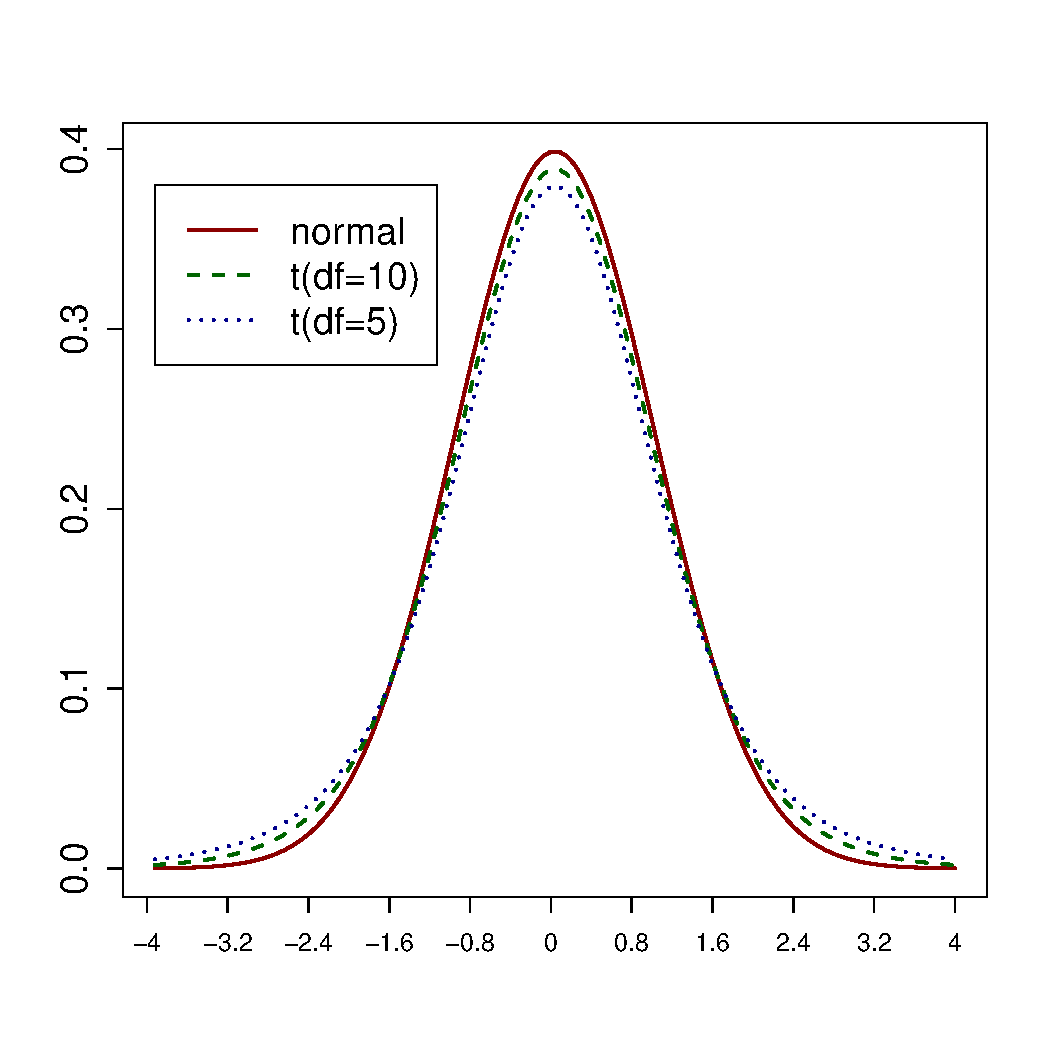
\includegraphics[width=0.5\textwidth]{graphics/tnorm}
    \end{center}
\end{frame}

% pdf("tnorm.pdf")
% plot(dnorm(x=seq(-4,4,length=100)), type="l", lwd=2, col="darkred", xlab="", ylab="", cex.axis=1.5, xaxt="n")
% axis(1,seq(0,100,length=11), labels=round(seq(-4,4,length=11), 2), cex=1.5)
% lines(dt(x=seq(-4,4,length=100), df=10), type="l", lwd=2, col="darkgreen", lty=2)
% lines(dt(x=seq(-4,4,length=100), df=5), type="l", lwd=2, col="darkblue", lty=3)
% legend(1,0.38,legend=c("normal","t(df=10)","t(df=5)"), col=c("darkred", "darkgreen","darkblue"), lty=c(1,2,3), lwd=2, cex=1.5)
% dev.off()

\begin{frame}
  {$df$ und Signifikanz}
  \begin{itemize}[<+->]
    \item \alert{$df=n-1$} ($\bar{x}$ muss für $s^s(x)$ bekannt sein)
    \item Welche t-Werte machen $1-\alpha$ der Werte aus?
    \item \texttt{> qt(c(0+0.05/2, 1-0.05/2), df=9)\\
      $\Rightarrow 2.262157 .. -2.262157$}
    \item Der errechnete t-Wert ist nicht signifikant.
    \item \Null: $\mu=\bar{x}$ nicht zurückgewiesen.
  \end{itemize}
\end{frame}

\begin{frame}
  {Effektstärke}
  \begin{itemize}[<+->]
    \item Signifikanz $\neq$ starker Effekt
    \item Effektstärke beim t-Test für Stichprobe $x$:
  \end{itemize}
  \pause
  \begin{center}
    \alert{Cohens $d=\frac{\bar{x}-\mu}{s(x)}$}
  \end{center}
  \pause
  \begin{itemize}
    \item Herleitung\slash Erklärung: Gravetter \& Wallnau, Kap.\ 9
  \end{itemize}
\end{frame}

\begin{frame}
  {Erklärung der Varianz}
  \begin{itemize}
    \item ähnlich der Effektstärke: \\
      \alert{Welcher Anteil der Varianz in den Daten\\
      wird durch die Unabhängige erklärt?}
  \end{itemize}
  \pause
  \begin{center}
    \alert{Cohens $r^2=\frac{t^2}{t^2+df}$}
  \end{center}
  \pause
  \begin{itemize}
    \item Herleitung\slash Erklärung: Gravetter \& Wallnau, Kap.\ 9
  \end{itemize}
\end{frame}

\subsection{t-Test mit zwei Stichproben}

\begin{frame}
  {Zwei-Stichproben t-Test}
  \begin{itemize}[<+->]
    \item \alert{zwei Grundgesamtheiten} (\zB dt.\ Sätze im 19.\ und im 20.\ Jh.)
    \item dazu: \alert{zwei Stichproben} (je eine) mit einem \alert{Mittelwert} (\zB Länge)
    \item Interesse: anhand der \alert{zwei Stichproben} zeigen,\\
      dass sie (sehr wahrscheinlich) \alert{aus zwei Grundgesamtheiten} kommen
    \item \alert{\Null: $\mu_1-\mu_0=0$}
    \item hier also: eine unabhängige Variable (Jahrhundert)\\
      und eine abhängige Variable (Satzlänge), gemessen als Mittel
  \end{itemize}
\end{frame}

\begin{frame}
  {Genereller Ansatz}
  Allgemein funktioniert der t-Test \alert{immer} so:
  \begin{center}
    \alert{$t=\frac{Stichprobenwert-Grundgesamtheitswert}{Standardfehler}$}
  \end{center}
  \pause
  Jetzt geht man per Hypothese von zwei GG und zwei Stichproben aus, also:
  \pause
  \begin{center}
    \alert{$t=\frac{(\bar{x_1}-\bar{x_2})-(\mu_1-\mu_2)}{SF(x_1-x_2)}$}
  \end{center}
  \pause
  \begin{itemize}[<+->]
    \item Wir testen also auf die \alert{Differenz der Unterschiede}.
    \item Per \Null\ wird gesetzt: \alert{$\mu_1-\mu_2=0$}
  \end{itemize} 
\end{frame}

\begin{frame}
  {Schätzung des Standardfehlers}
  Für \alert{gleichgroße Stichproben}:
  \begin{center}
    \alert{$SF(\bar{x_1}-\bar{x_2})=\sqrt{\frac{s^2(x_1)}{n_1}+\frac{s^2(x_2)}{n_2}}$}
  \end{center}
  \pause
  \begin{itemize}[<+->]
    \item Problem: Beitrag zum SF von beiden Stichproben gleich.
    \item Besser: \alert{zusammengefasste Varianz}, und daraus dann SF.
  \end{itemize}
  \pause
  \begin{center}
    \alert{$s^2_p(x_1,x_2)=\frac{(\sum\limits_{i=1}^{n}(x_{1,i}-\bar{x_1})^2)+(\sum\limits_{i=1}^{n}(x_{2,i}-\bar{x_2})^2)}{(n_1-1)+(n_2-1)}=\frac{SQ(x_1)+SQ(x_2)}{(n_1-1)+(n_2-1)}$}\\
    \vspace{0.5cm}
    \pause
    \alert{$SF(x_1-x_2)=\sqrt{\frac{s^2_p(x_1,x_2)}{n_1}+\frac{s^2_p(x_1,x_2)}{n_2}}$}
  \end{center}
  \pause
  \footnotesize
  Mehr: Gravetter \& Wallnau, Kap.\ 10
\end{frame}

\begin{frame}
  {Illustration der zusammengefassten Varianz}
  \begin{center}
    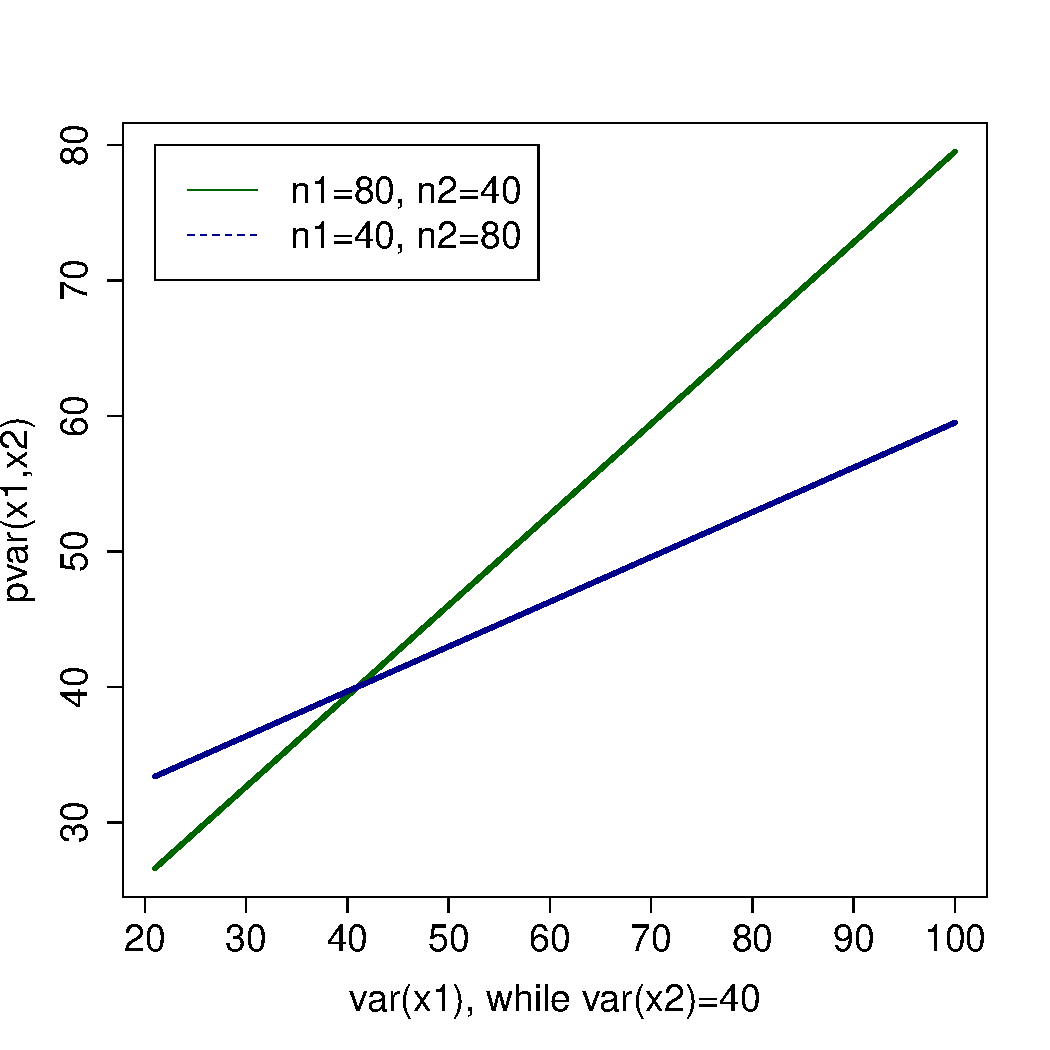
\includegraphics[width=0.5\textwidth]{graphics/pvar}
  \end{center}
\end{frame}

% pdf("pvar.pdf")
% plot(apply(vars1, 1, pv), type="l", lwd=3, cex=1.5, cex.axis=1.5, xlab="var(x1), while var(x2)=40", cex.lab=1.5, ylab="pvar(x1,x2)", col="darkgreen", xaxt="n")
% axis(1, at=seq(0,80,by=10), labels=seq(20,100,by=10), cex.axis=1.5)
% lines(apply(vars2, 1, pv), lwd=3, col="darkblue")
% legend(1,80,legend=c("n1=80, n2=40", "n1=40, n2=80"), lty=c(1,2), col=c("darkgreen", "darkblue"), cex=1.5)
% dev.off()

\begin{frame}
  {Rechnen des Tests}
  t-Wert
  \begin{center}
    \alert{$t=$}$\frac{(\bar{x_1}-\bar{x_2})-(\mu_1-\mu_2)}{SF(x_1-x_2)}=\frac{(\bar{x_1}-\bar{x_2})-0}{SF(x_1-x_2)}=$\alert{$\frac{\bar{x_1}-\bar{x_2}}{SF(x_1-x_2)}$}
  \end{center}
  \pause
  Freiheitsgrade
  \begin{center}
    $df=df(x_1)+df(x_2)=(n_1-1)+(n_2-1)$
  \end{center}
  \pause
  Effektstärke
  \begin{center}
    $d=\frac{\bar{x_1}-\bar{x_2}}{\sqrt{s^2_p}}$
  \end{center}
  \pause
  Erklärung der Varianz
  \begin{center}
    $r^2=\frac{t^2}{t^2+df}$
  \end{center}
\end{frame}

\begin{frame}
  {Übung}
  Bitte "`von Hand in \texttt{R}"' t-Test für folgende zwei Stichproben\\
  bei $\alpha=0.05$ rechnen:\\
  \begin{center}
    $x_1=[11, 11, 8, 8, 11, 9, 8, 11, 9, 8]$\\
    $x_2=[10, 14, 14, 13, 11, 14, 10, 14, 12, 10]$
  \end{center}
  \pause
  \begin{center}
    Und überprüfen mit:\\
    \texttt{> t.test(x1, x2)}
  \end{center}
\end{frame}

\begin{frame}
  {Voraussetzungen prüfen I}
  Die \alert{GGs müssen normalerverteilt} sein:
  \begin{center}
    \texttt{shapiro.test(x)}\\
    Wenn $p\leq0.05$ wird die Nullhypothese des Shapiro-Wilk-Tests verworfen --\\
    \Null: Die Werte stammen aus einer normalverteilten GG.
  \end{center}
  \pause
  Die \alert{Varianzen müssen homogen sein}:
  \begin{center}
    \texttt{var.test(x1, x2)}\\
    Auch hier: $p\leq0.05$ weist die \Null\ zurück (sehr informell) --\\
    \Null: Die Varianzen von x1 und x2 sind homogen.
  \end{center}
\pause
\begin{center}
  \alert{Solche Tests sind umstritten, weil sie i.\,d.\,R.\ viel zu empfindlich reagieren.\\
    \citet{ZuurEa2009} empfehlen \zB grafische Methoden (bei linearen Modellen).}
\end{center}

\end{frame}


\begin{frame}
  {Voraussetzungen prüfen II}
  Wenn Voraussetzungen nicht erfüllt sind:
  \begin{itemize}[<+->]
    \item steigt das Risiko für Typ 1-Fehler
    \item nicht-parametrische Alternative nehmen
    \item Daten transformieren
    \item sich über Robustheit des Test ggü. verletzten Annahmen informieren\\
      (oft schwer zugängliche und kontroverse Spezialliteratur)
  \end{itemize}
\end{frame}


\ifdefined\TITLE
  \section{Nächste Woche | Überblick}

  \begin{frame}
    {Einzelthemen}
    \begin{enumerate}
      \item Inferenz
      \item Deskriptive Statistik
      \item Nichtparametrische Verfahren
      \item z-Test und t-Test
      \item \alert{ANOVA}
      \item Freiheitsgrade und Effektstärken
      \item Power und Severity
      \item Lineare Modelle
      \item Generalisierte Lineare Modelle
      \item Gemischte Modelle
    \end{enumerate}
  \end{frame}
\fi


  \let\subsection\section\let\section\woopsi
  
  \section{Simulationen}

  \section{ANOVA}
  \let\woopsi\section\let\section\subsection\let\subsection\subsubsection
  \section{ANOVA}

\begin{frame}
  {Übersicht}
  \begin{itemize}[<+->]
    \item Vergleiche von Mittelwerten zwischen mehr als zwei Gruppen
    \item Mittelwertvergleiche mit mehreren Unabhängigen
    \item \alert{Warum kann man über Varianzen Mittelwerte vergleichen?}
  \end{itemize}
\end{frame}

\begin{frame}
  {Literatur}
  \begin{itemize}
    \item \citet{GravetterWallnau2007}
    \item \citet{Bortz2010}
    \item indirekt: \citet{MaxwellDelaney2004}
  \end{itemize}
\end{frame}

\subsection{Überblick}

\begin{frame}
  {Mittelwerte und Varianzen}
  \begin{itemize}[<+->]
    \item Einschränkung beim t-test: immer nur 2 Gruppen
    \item t-Test bei mehr als 2 Gruppen: komplizierte paarweise Vergleiche
      \Zeile
    \item stattdessen ANOVA: ANalysis Of VAriance
    \item Vergleich von Varianzen zwischen beliebigen Gruppen
    \item Schluss auf Mittelwerte nur indirekt über die Varianzen
      \Zeile
    \item \alert{bei zwei Gruppen: Konvergenz von t-Test und ANOVA}
  \end{itemize}
\end{frame}

\begin{frame}
  {Achtung: Gruppen vs.\ Faktoren}
  \begin{itemize}[<+->]
    \item ANOVA vergleicht immer \alert{mehrere Gruppen}
    \item Gruppen bei der einfaktoriellen ANOVA =\\
      den Ausprägungen \alert{einer unabhängigen Variable} (\zB Text-Register)
    \item diese Variablen heißen hier \alert{Faktoren}.
      \Zeile
    \item Einfluss der Faktoren auf \alert{eine abhängige} (\zB Satzlänge, Lesezeit)
      \Zeile
    \item bei mehreren Faktoren (\zB Text-Register und Jahrhundert):\\
      \alert{mehrfaktorielle ANOVA}.
  \end{itemize}
\end{frame}

\begin{frame}
  {Idee bei ANOVA (\zB drei Gruppen)}
  \begin{itemize}[<+->]
    \item \alert{H0: $\bar{x_1}=\bar{x_2}=\bar{x3}$}
    \item aber: \alert{Es gibt keinen ``Differenzwert'' für drei Mittel}\\
      (also sowas wie den t-Wert).
      \Zeile
    \item daher \alert{Varianzvergleich}
    \item \alert{F-Wert} (Verteilung unter H0 bekannt) als Test-Statistik
  \end{itemize}
  \pause
  \vspace{0.5cm}
  \begin{center}
    \alert{$F=\frac{\mathsf{Varianz\ zwischen\ Stichprobenmitteln}}{\mathsf{Varianz\ in\ den\ Stichproben}}=\frac{\mathsf{Varianz\ zwischen\ Stichprobenmitteln}}{\mathsf{Varianz\ per\ Zufall}}$}
  \end{center}
\end{frame}


\subsection{Graphische Einführung}

\begin{frame}
  {Drei Stichproben}
  $x_1=[0, 1, 3, 1, 0]$\\
  $x_2=[4, 3, 6, 3, 4]$\\
  $x_3=[1, 2, 2, 0, 0]$\\

  \vspace{-0.5cm}
  \begin{center}
    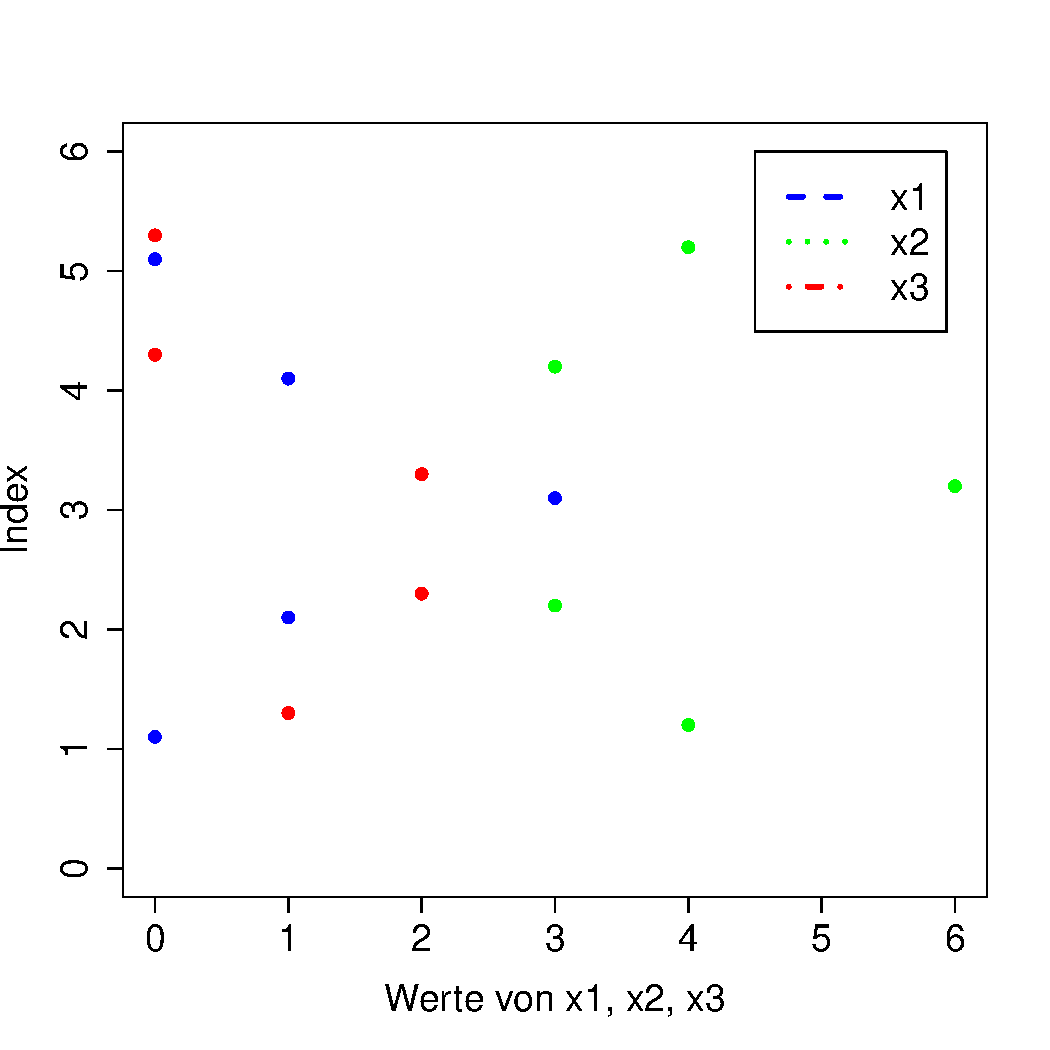
\includegraphics[width=0.45\textwidth]{anova_points}
  \end{center}
\end{frame}


\begin{frame}
  {Komponenten der Varianz von $x_1$}
  
  \begin{center}
    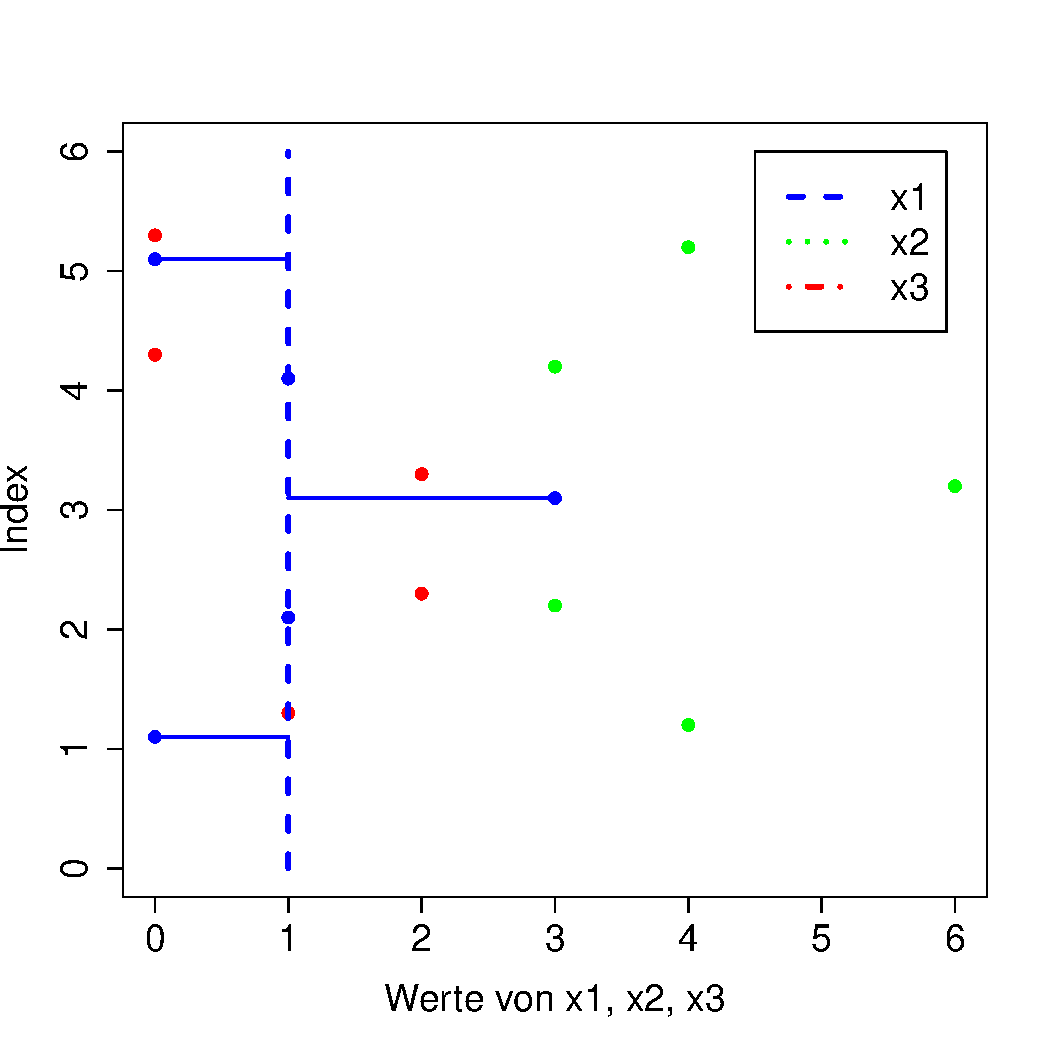
\includegraphics[width=0.45\textwidth]{anova_var_x1}\\
    $s^2(x_1)=1.5$
  \end{center}
\end{frame}

\begin{frame}
  {Komponenten der Varianz von $x_2$}
  
  \begin{center}
    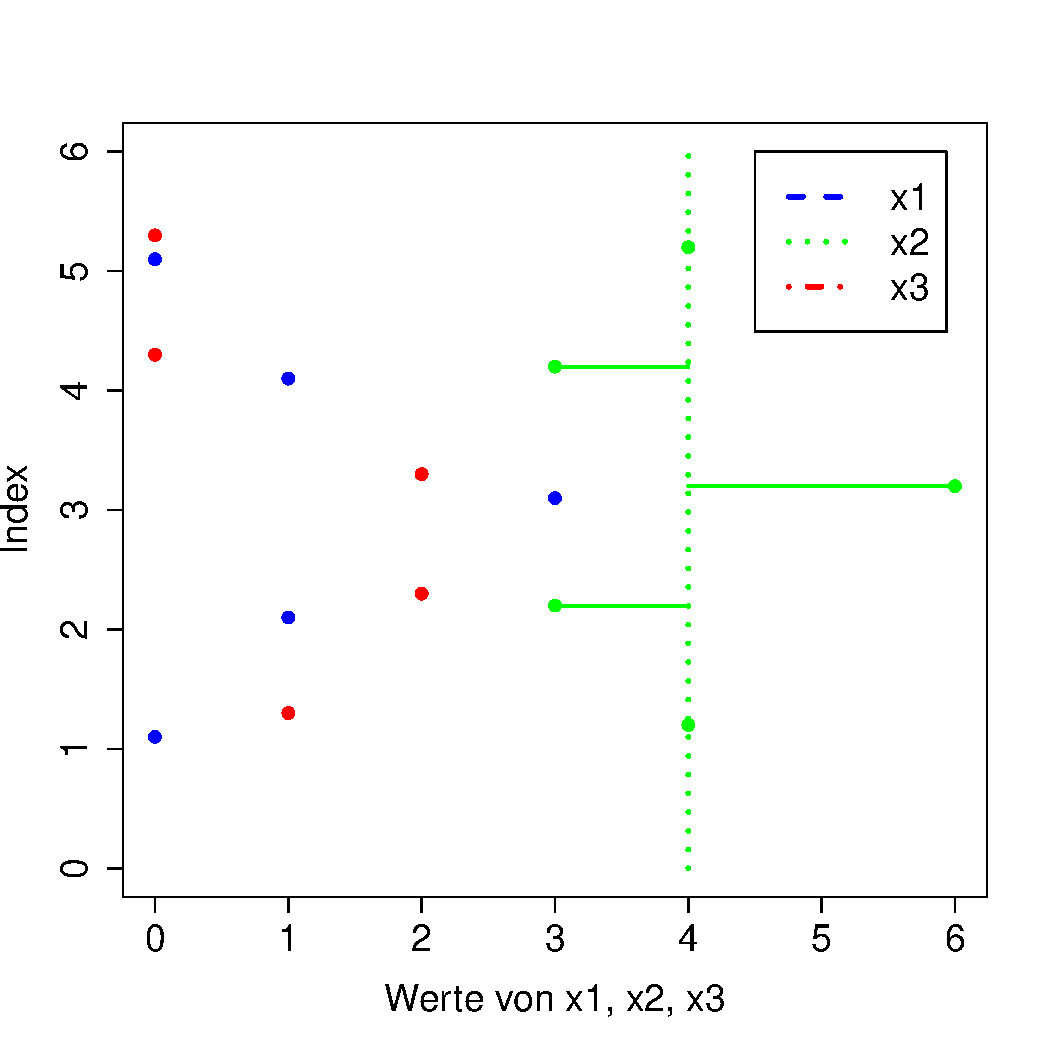
\includegraphics[width=0.45\textwidth]{anova_var_x2}\\
    $s^2(x_2)=1.5$
  \end{center}
\end{frame}

\begin{frame}
  {Komponenten der Varianz von $x_3$}
  
  \begin{center}
    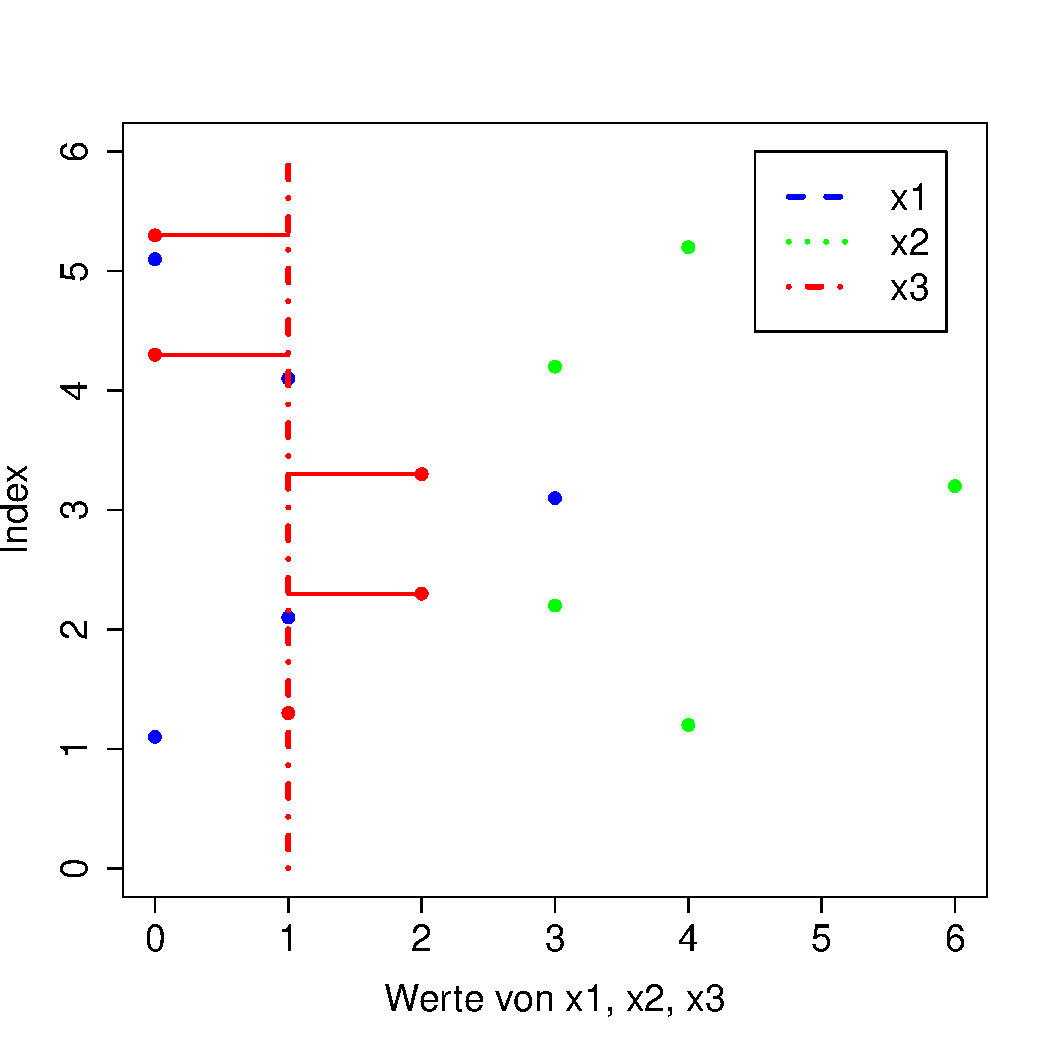
\includegraphics[width=0.45\textwidth]{anova_var_x3}\\
    $s^2(x_3)=1$
  \end{center}
\end{frame}

\begin{frame}
  {Varianz in der zusammengefassten Stichprobe $X$}
  
  \begin{center}
    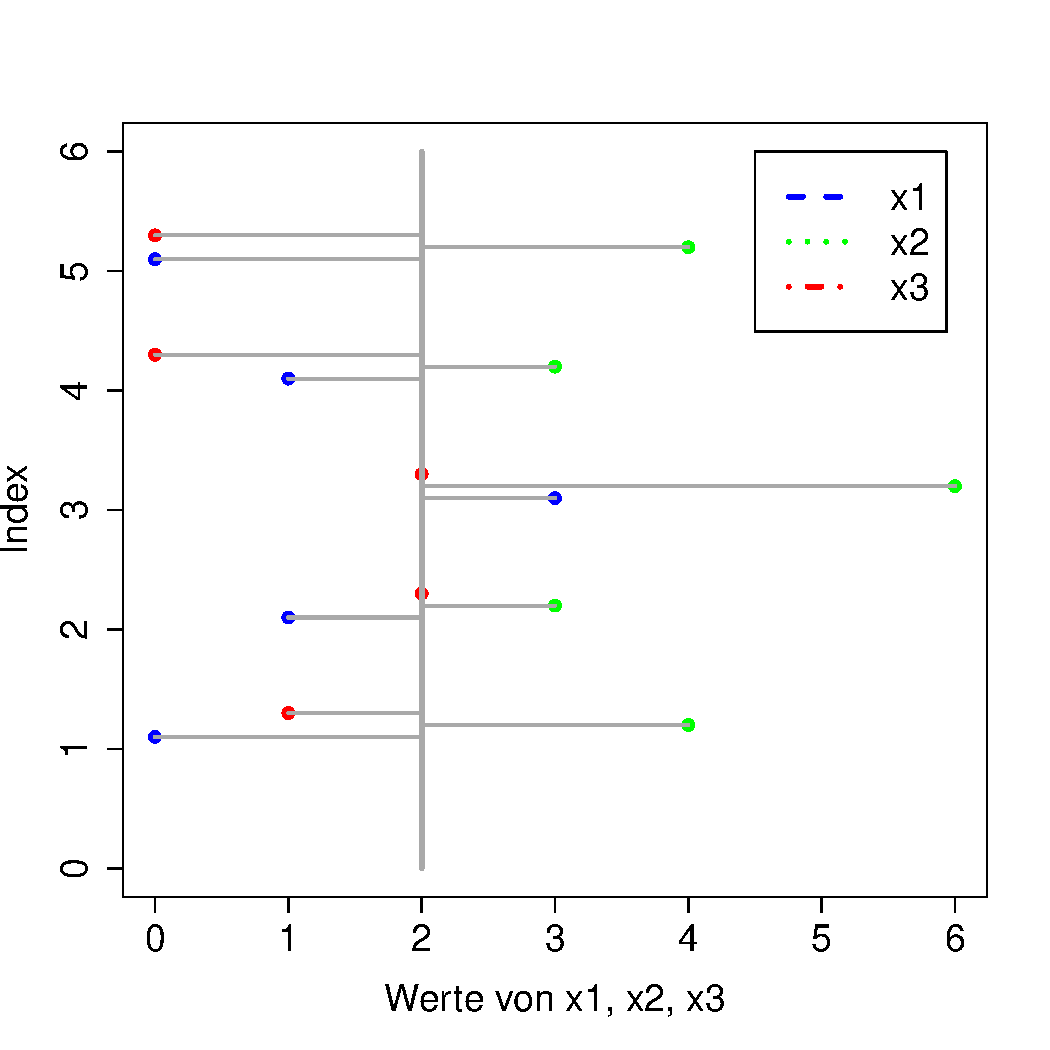
\includegraphics[width=0.45\textwidth]{anova_var_total}\\
    $s^2(X)=3.29$
  \end{center}
\end{frame}

\begin{frame}
  {Varianz zwischen den drei Gruppen}
  
  \begin{center}
    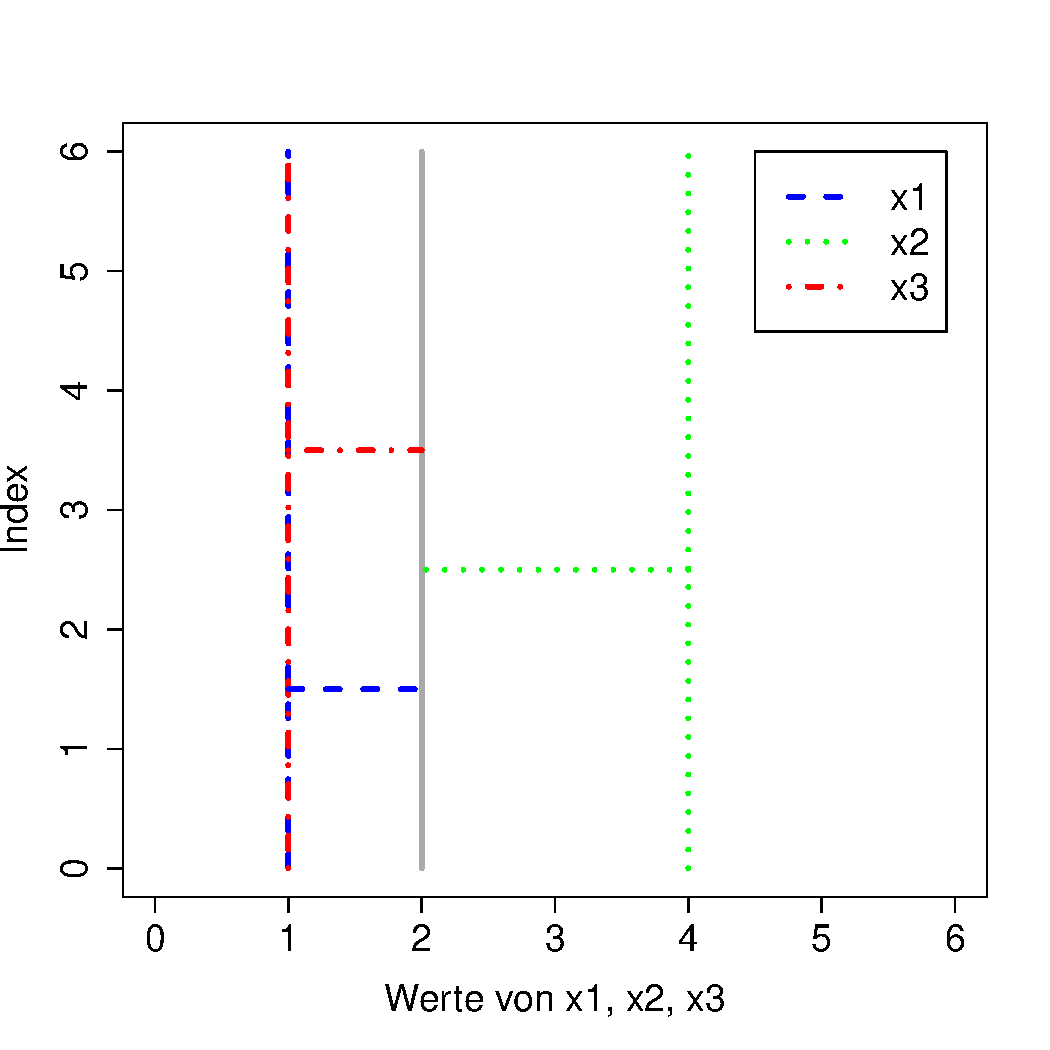
\includegraphics[width=0.45\textwidth]{anova_var_between}\\
    $s^2([\bar{x_1}, \bar{x_2}, \bar{x_3}])=1.33$\\
    \vspace{0.5cm}
    Achtung: Bei unterschiedlichen Stichprobengrößen\\
    ist das nicht ganz so einfach!
  \end{center}
\end{frame}


\begin{frame}
  {Es gilt bezüglich der Varianzen}

  \begin{center}
    \begin{tabular}[h!]{ccccc}
      \multirow{3}{*}{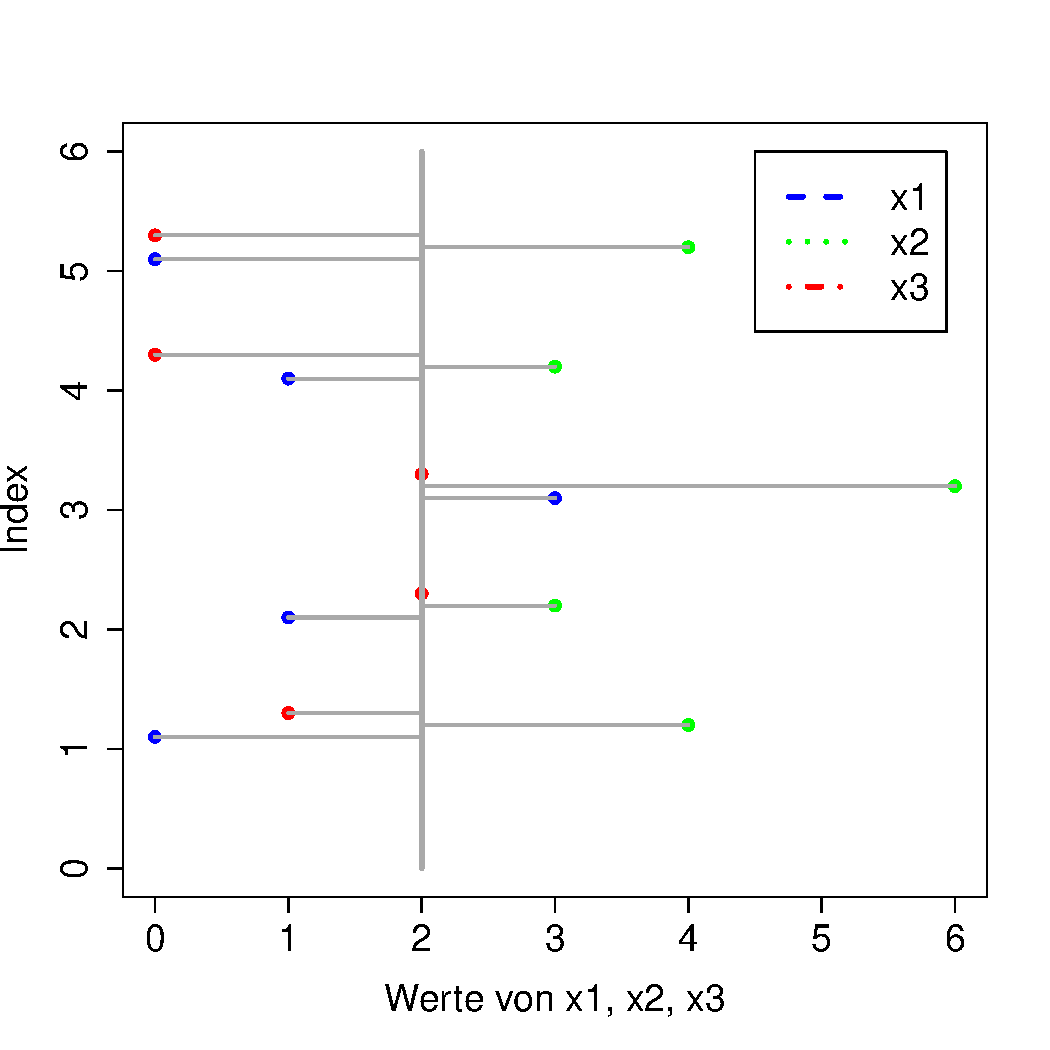
\includegraphics[width=0.2\textwidth]{anova_var_total}} & \multirow{3}{*}{$=$} & \multirow{3}{*}{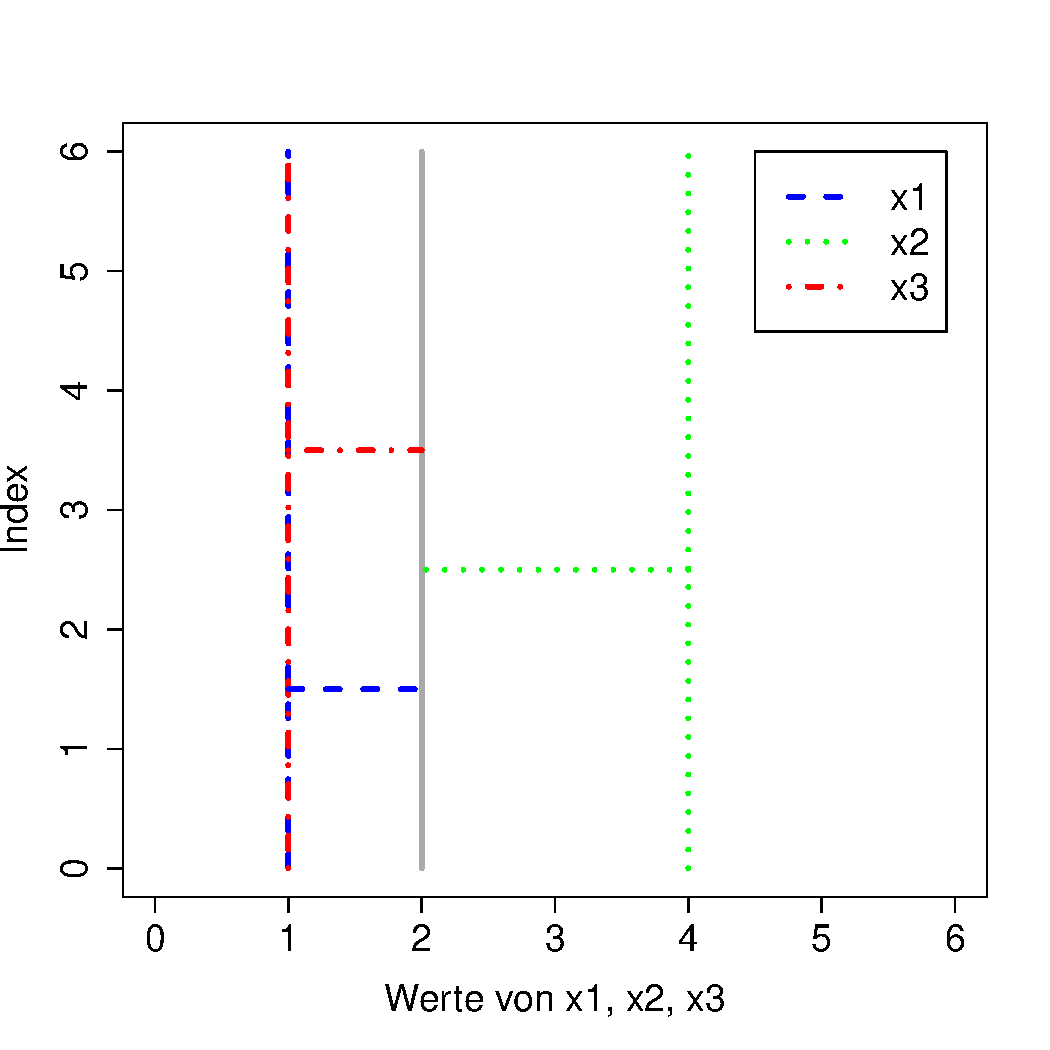
\includegraphics[width=0.2\textwidth]{anova_var_between}} & \multirow{3}{*}{$+$} & 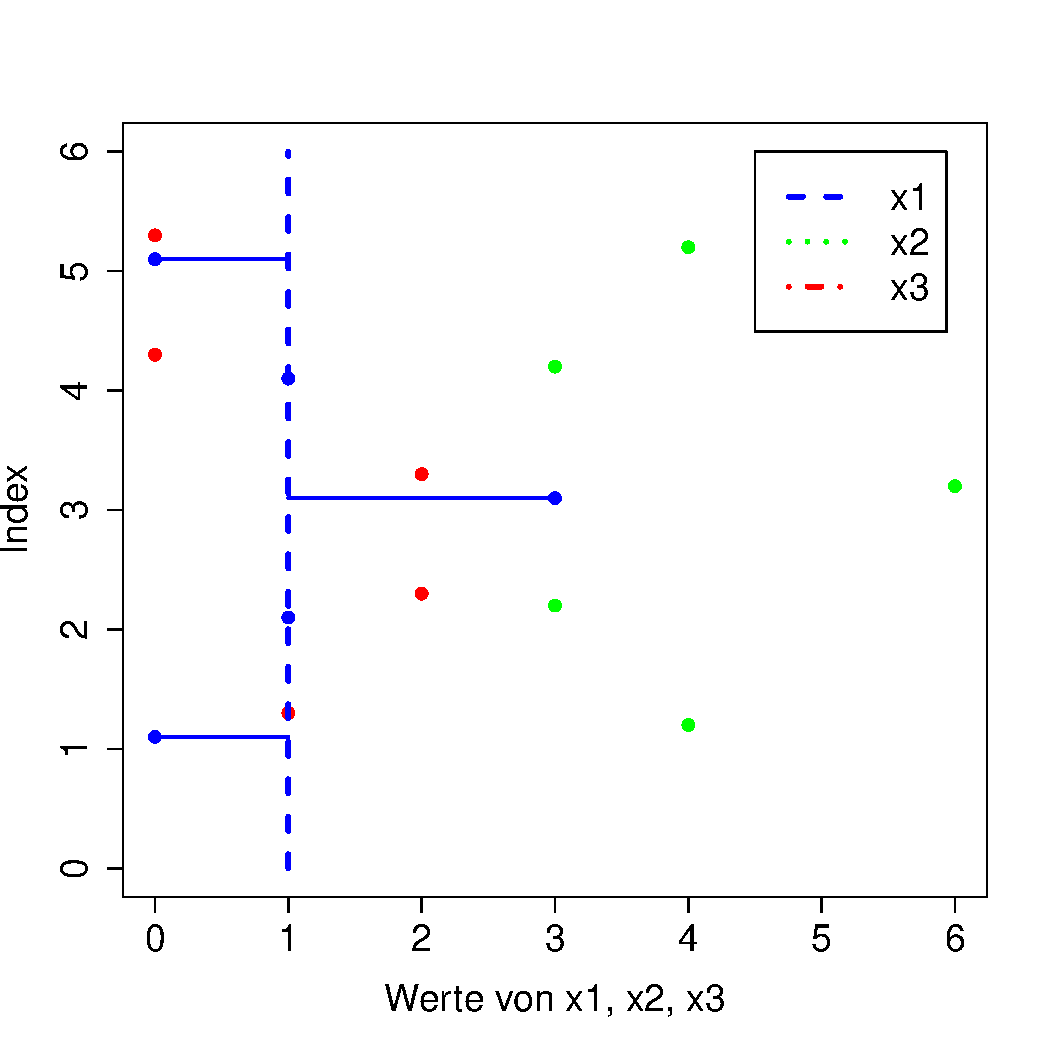
\includegraphics[width=0.15\textwidth]{anova_var_x1} \\
      &&&& 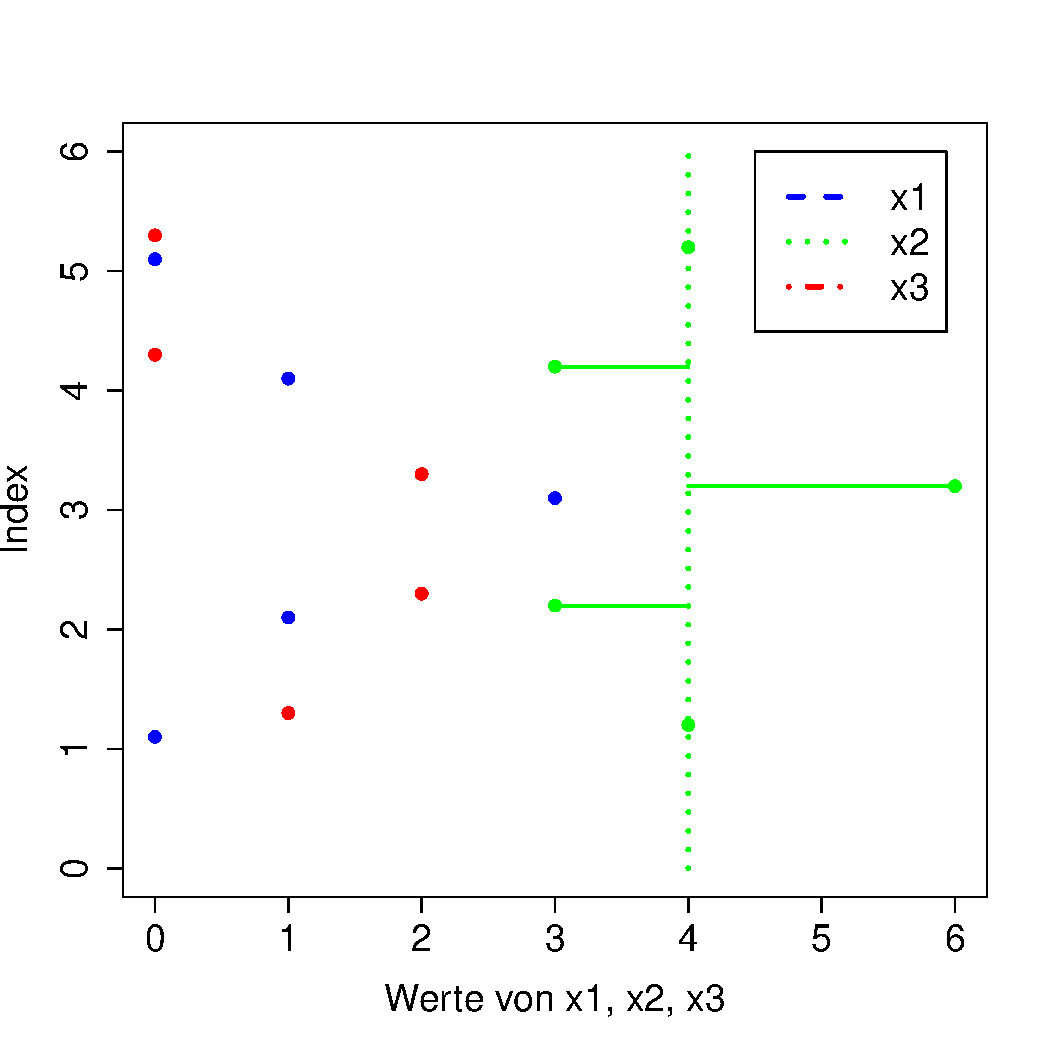
\includegraphics[width=0.15\textwidth]{anova_var_x2} \\
      &&&& 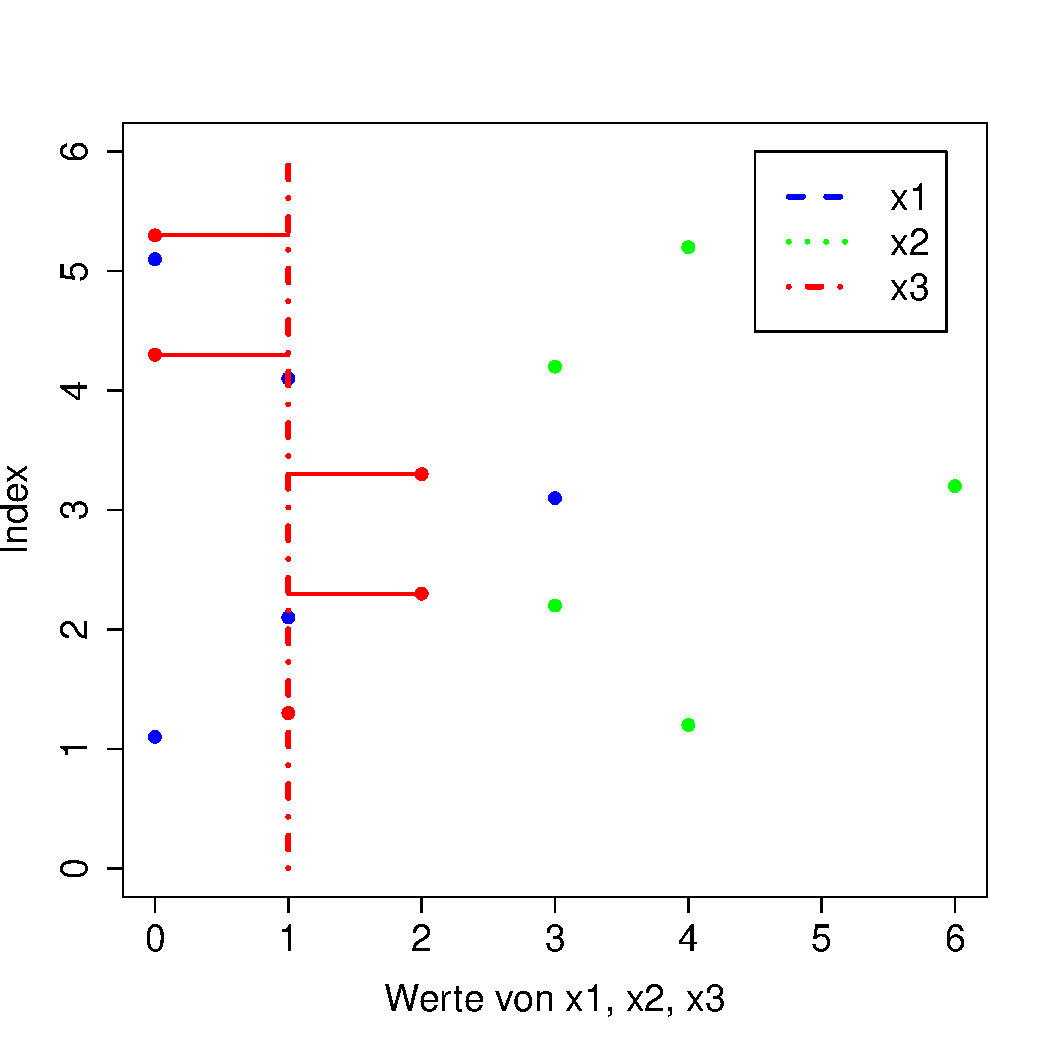
\includegraphics[width=0.15\textwidth]{anova_var_x3} \\
      \hline
      $s^2(X)$ & $=$ & $s^2(\bar{x_1},\bar{x_2},\bar{x_3})$ & $+$ & $s^2(x_1)+s^2(x_2)+s^2(x_3)$ \\
    \end{tabular}\\
    \Zeile
    \rot{Wenn man den Abstand zwischen den Mitteln verschiebt,\\\textbf{muss} die Gesamtvarianz größer werden!}
  \end{center}
\end{frame}

\begin{frame}
  {Graphische Verdeutlichung des F-Werts}
  
  \begin{center}
    \alert{$F=\frac{\mathsf{Varianz\ zwischen\ Stichprobenmitteln}}{\mathsf{Varianz\ in\ den\ Stichproben}}=\frac{\mathsf{Varianz\ zwischen\ Stichprobenmitteln}}{\mathsf{Varianz\ per\ Zufall}}$}\\
    \begin{tabular}[h!]{cc}
      \multirow{2}{*}{$F=$} & 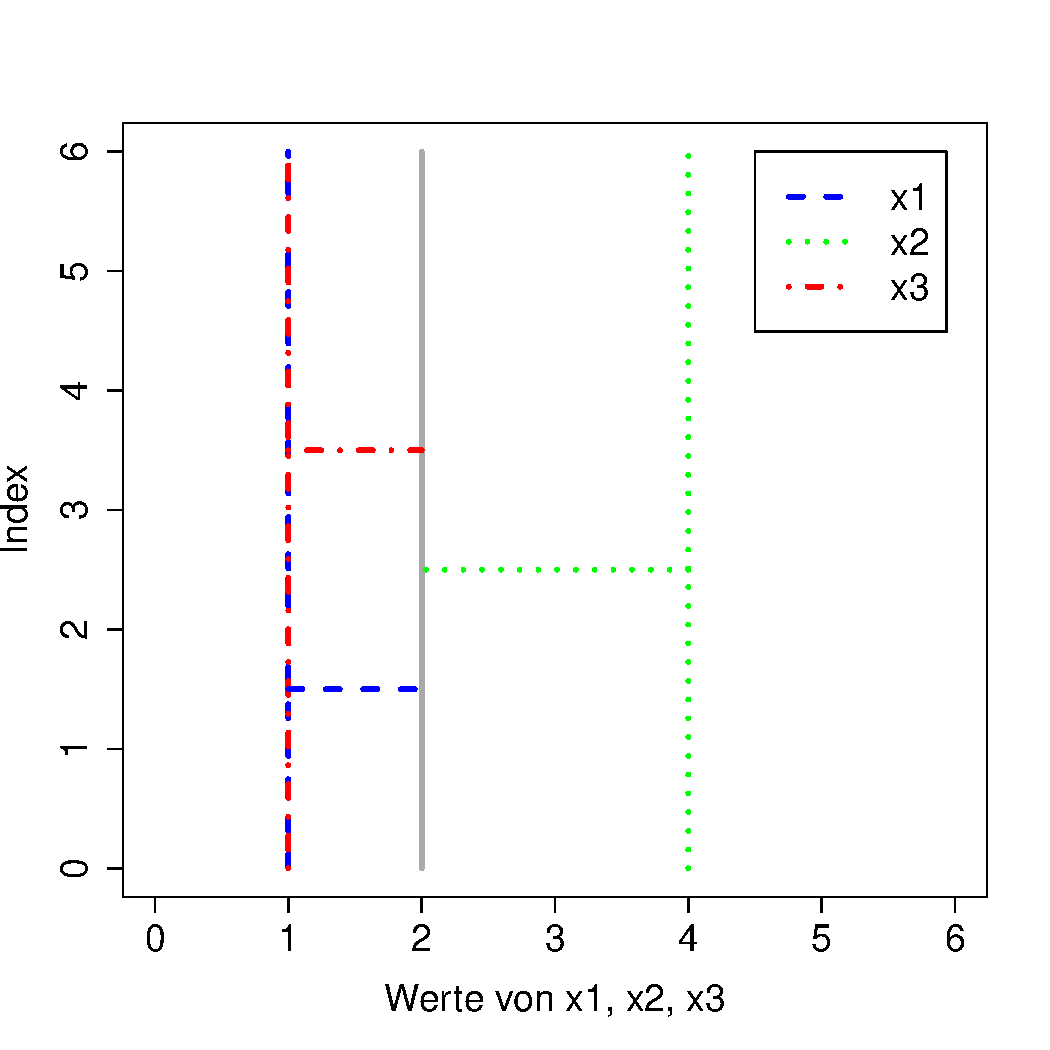
\includegraphics[width=0.2\textwidth]{anova_var_between} \\\cline{2-2}
      & 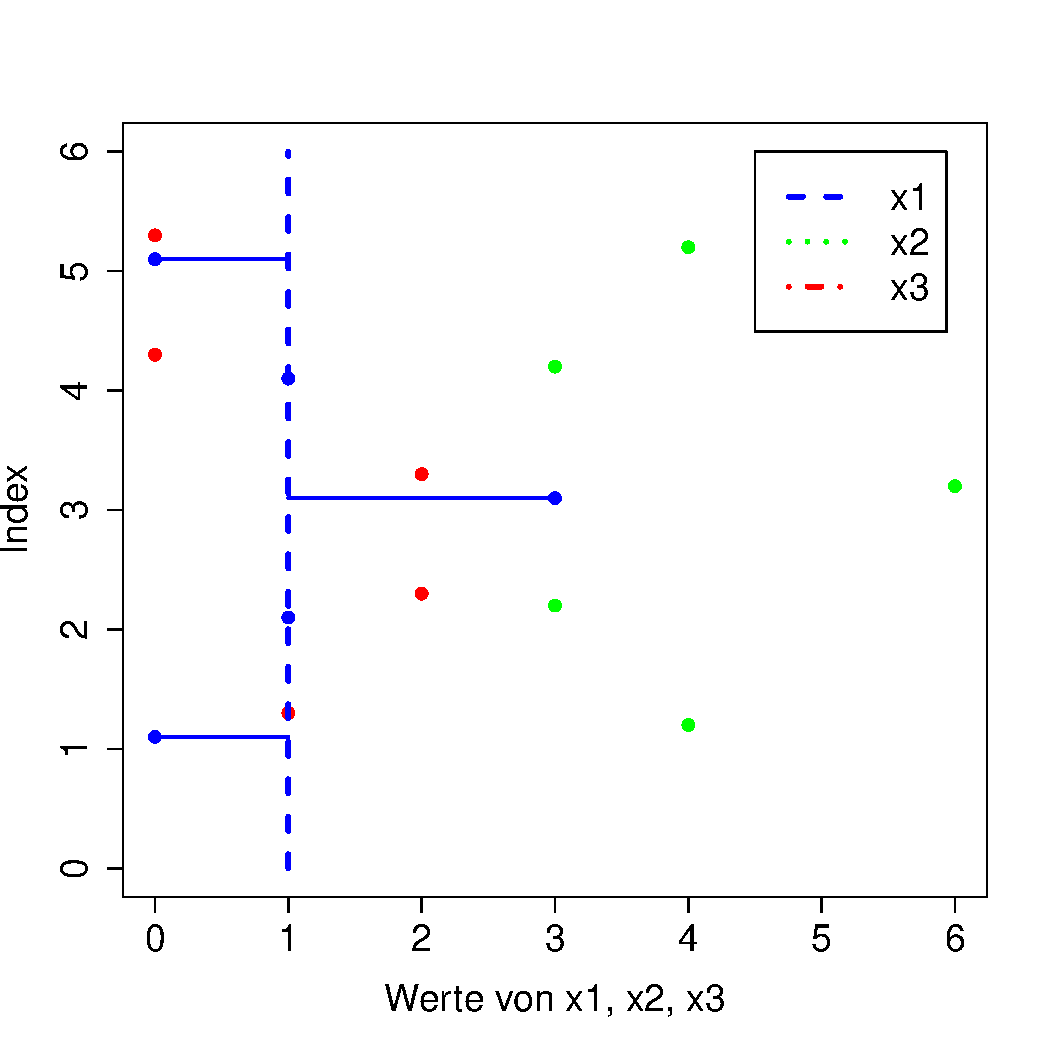
\includegraphics[width=0.2\textwidth]{anova_var_x1}\ \raisebox{1.25cm}{+}\ 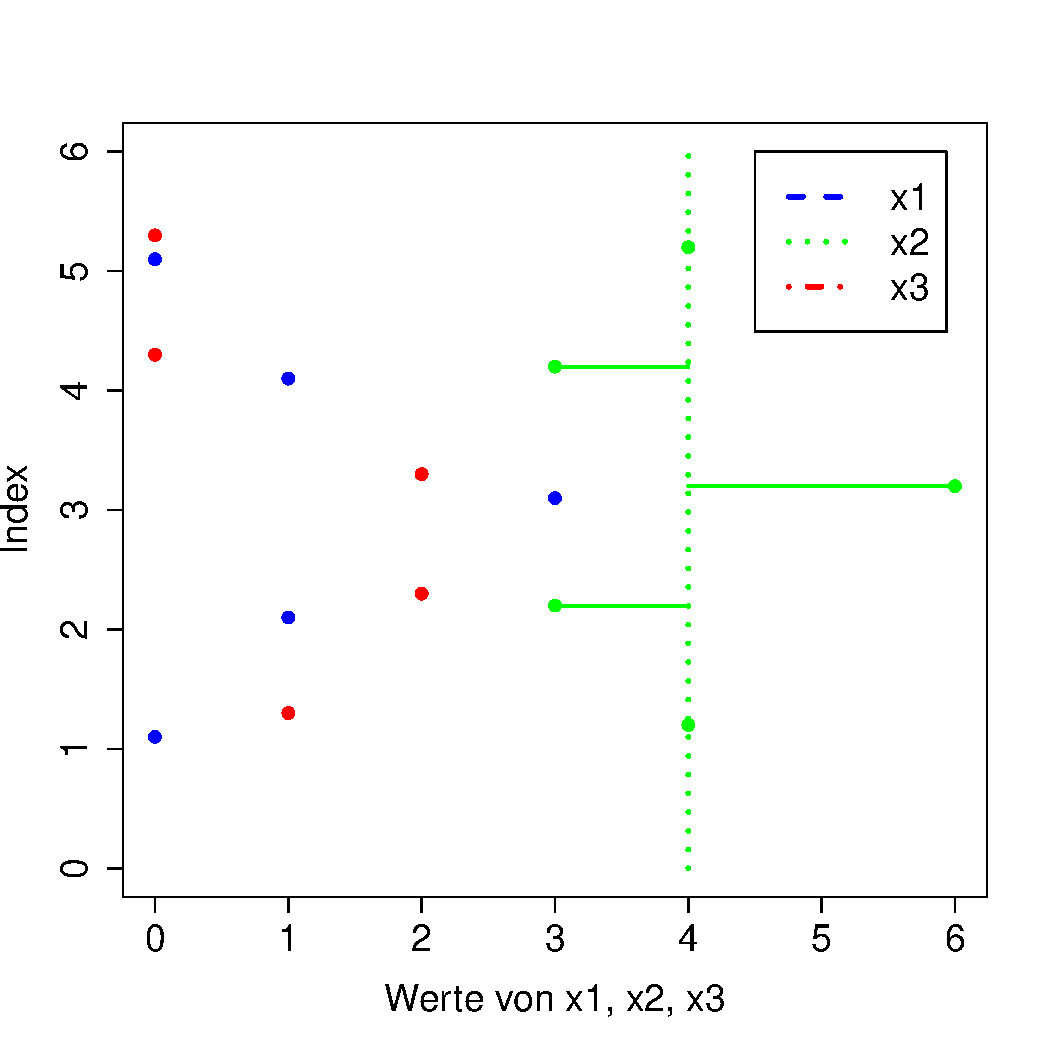
\includegraphics[width=0.2\textwidth]{anova_var_x2}\ \raisebox{1.25cm}{+}\ 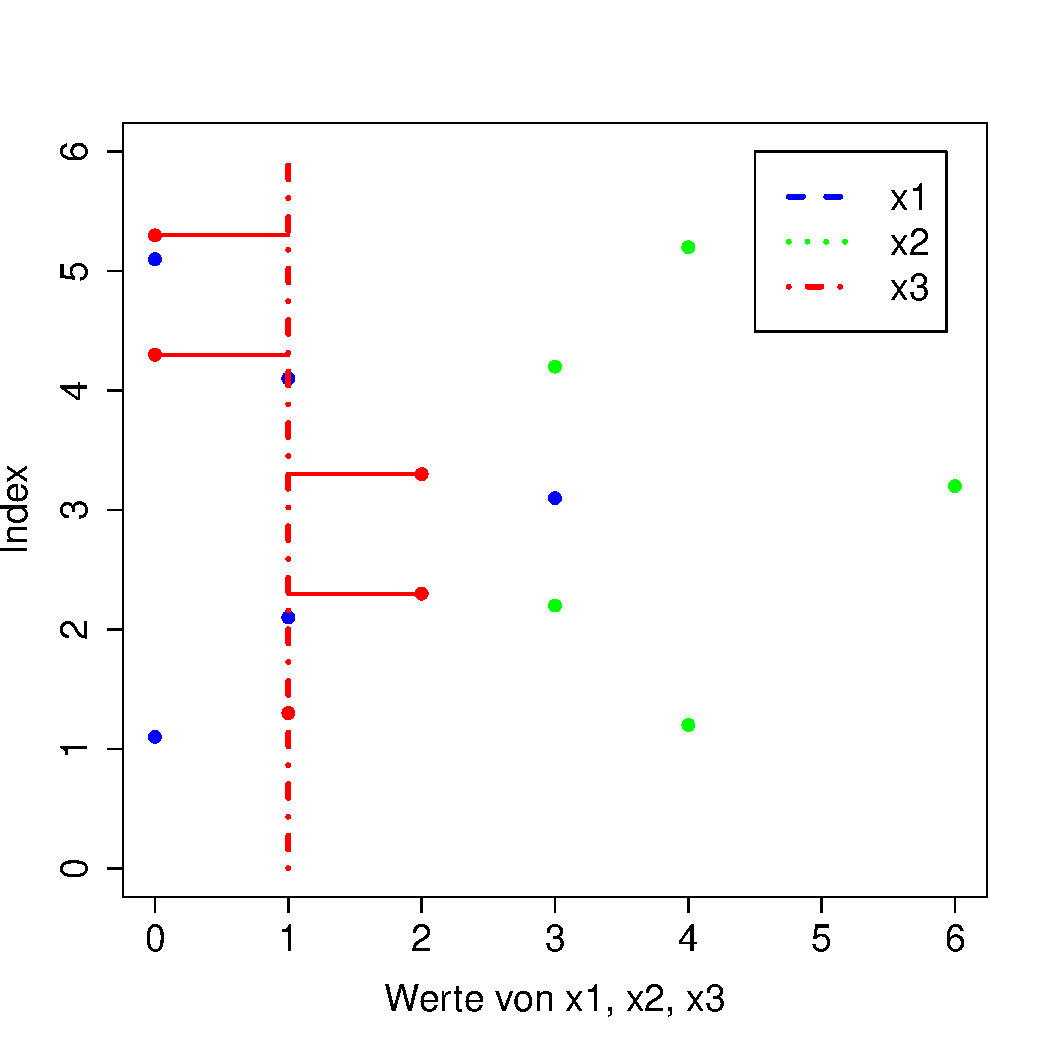
\includegraphics[width=0.2\textwidth]{anova_var_x3} \\
    \end{tabular}\\
    \Zeile
    \rot{Wenn man den Abstand zwischen den Mitteln verschiebt,\\\textbf{muss} die Gesamtvarianz größer werden!}
  \end{center}
\end{frame}

\subsection{Einfaktorielle ANOVA}

\begin{frame}
  {Wie funktioniert der F-Wert}
  \begin{itemize}[<+->]
    \item $F=\frac{\mathsf{Varianz\ zwischen\ Stichprobenmitteln}}{\mathsf{Varianz\ in\ den\ Stichproben}}$
    \Zeile
    \item Warum?
    \item $F=\frac{\mathsf{\alert{Unterschied\ durch\ Effekt}+Unterschiede\ durch\ restliche\ Varianz}}{\mathsf{Unterschied\ durch\ restliche\ Varianz}}$
    \Zeile
    \item Unter Annahme der H0 gibt es keinen Effekt, \ldots
    \item also \alert{$Unterschied\ durch\ Effekt=0$}
    \Zeile
    \item dann: $F=\frac{\mathsf{\alert{0}+Unterschiede\ durch\ restliche\ Varianz}}{\mathsf{Unterschied\ durch\ restliche\ Varianz}}=\alert{1}$
  \end{itemize}
\end{frame}

\begin{frame}
  {Notation, fast wie in Gravetter \& Wallnau, Kap.~13}
  \begin{itemize}[<+->]
    \item Anzahl der Gruppen \alert{$x_i$}: \alert{$k$}
    \item Größe der Gruppen: \alert{$n_i$}
    \item Größe der Gesamtstichprobe \alert{$X$}: \alert{$N$}
    \item Summen der Gruppen: \alert{$T_i$}
    \item Gesamtsumme: \alert{$G$}
    \item Mittel (anders als G\&W): \alert{$\bar{x_i}$}, \alert{$\bar{X}$}
    \item Summe der Quadrate (=Zähler der Varianz): \alert{$SQ(x_i)$}, \alert{$SQ(X)$}
  \end{itemize}
  \pause
  \vspace{0.5cm}
  Zur Erinnerung: $s^2(x)=\frac{\sum (x-\bar{x})}{n-1}=\frac{SQ(x)}{df(x)}$\\
\end{frame}

\begin{frame}
  {Varianz ist Varianz beim F-Wert}
  \begin{center}
    $F=\frac{Varianz\ zwischen\ den\ Gruppen}{Varianz\ in\ den\ Gruppen}=\frac{\ \ \ s^2_{zwischen}\ \ \ }{s^2_{in}}=\alert{\frac{\ \ \ \frac{SQ_{zwischen}}{df_{zwischen}}\ \ \ }{\frac{SQ_{in}}{df_{in}}}}$\\
    \vspace{0.5cm}

    denn\\
    \vspace{0.5cm}

    $s^2(x)=\frac{SQ(x)}{df(x)}$
  \end{center}
\end{frame}

\begin{frame}
  {Berechnung der SQ}
  Am einfachsten unter Beachtung von:\\
  \alert{$SQ_{gesamt}=SQ_{zwischen}+SQ_{in}$}\\

  \vspace{0.5cm}
  \pause
  Es gilt: \alert{$SQ_{gesamt}=SQ(X)=\sum(X-\bar{X})$}\\
  
  \vspace{0.5cm}
  \pause
  Außerdem: \alert{$SQ_{in}=\sum SQ(x_i)$}\\
  
  \vspace{0.5cm}
  \pause
  Damit: \alert{$SQ_{zwischen}=SQ_{gesamt}-SQ_{in}$}\\
\end{frame}

\begin{frame}
  {$SQ_{zwischen}$}
  $SQ_{zwischen}$ kann man auch direkt ausrechnen:

  \vspace{0.5cm}
  \begin{center}
    $SQ_{zwischen}=\sum\limits_i(\frac{T_i^2}{n_i})-\frac{G^2}{N}$
  \end{center}
\end{frame}


\begin{frame}
  {Aufgabe}
  $x_1=[0, 1, 3, 1, 0]$\\
  $x_2=[4, 3, 6, 3, 4]$\\
  $x_3=[1, 2, 2, 0, 0]$\\

  \begin{center}
    Bitte alle $SQ$ ausrechnen, inkl.\ $SQ_{zwischen}$ direkt.
  \end{center}

  \vspace{0.5cm}
  \scriptsize
  Tipp: Sie brauchen als Vorwissen \alert{nur}\\
  den Stoff der ersten Statistik-Sitzung:
  \begin{itemize}
    \item arithmetisches Mittel
    \item SQ
  \end{itemize}
\end{frame}

\begin{frame}
  {Freiheitsgrade ausrechnen}
  Es gilt auch hier, ähnlich wie bei den $SQ$:\\
  \alert{$df_{gesamt}=df_{zwischen}+df_{in}$}

  \vspace{0.5cm}
  $df_{gesamt}=N-1$\\[2ex]
  $df_{zwischen}=k-1$\\[2ex]
  $df_{in}=\sum\limits_{i=1}^{k}(n_i-1)=(N-1)-(k-1)$
\end{frame}

\begin{frame}
  {Alles zusammen: F-Wert}
  \begin{center}
    $F=\frac{s^2_{zwischen}}{s^2_{in}}=\frac{\ \ \ \frac{SQ_{zwischen}}{df_{zwischen}}\ \ \ }{\frac{SQ_{in}}{df_{in}}}$\\
  \end{center}

  \vspace{0.5cm}
  \begin{center}
    Bitte ausrechnen für o.\,g.\ Beispiel.
  \end{center}
\end{frame}

\begin{frame}
  {Ermitteln der kritischen Werte}
  \begin{center}
    F-Verteilung:\\
    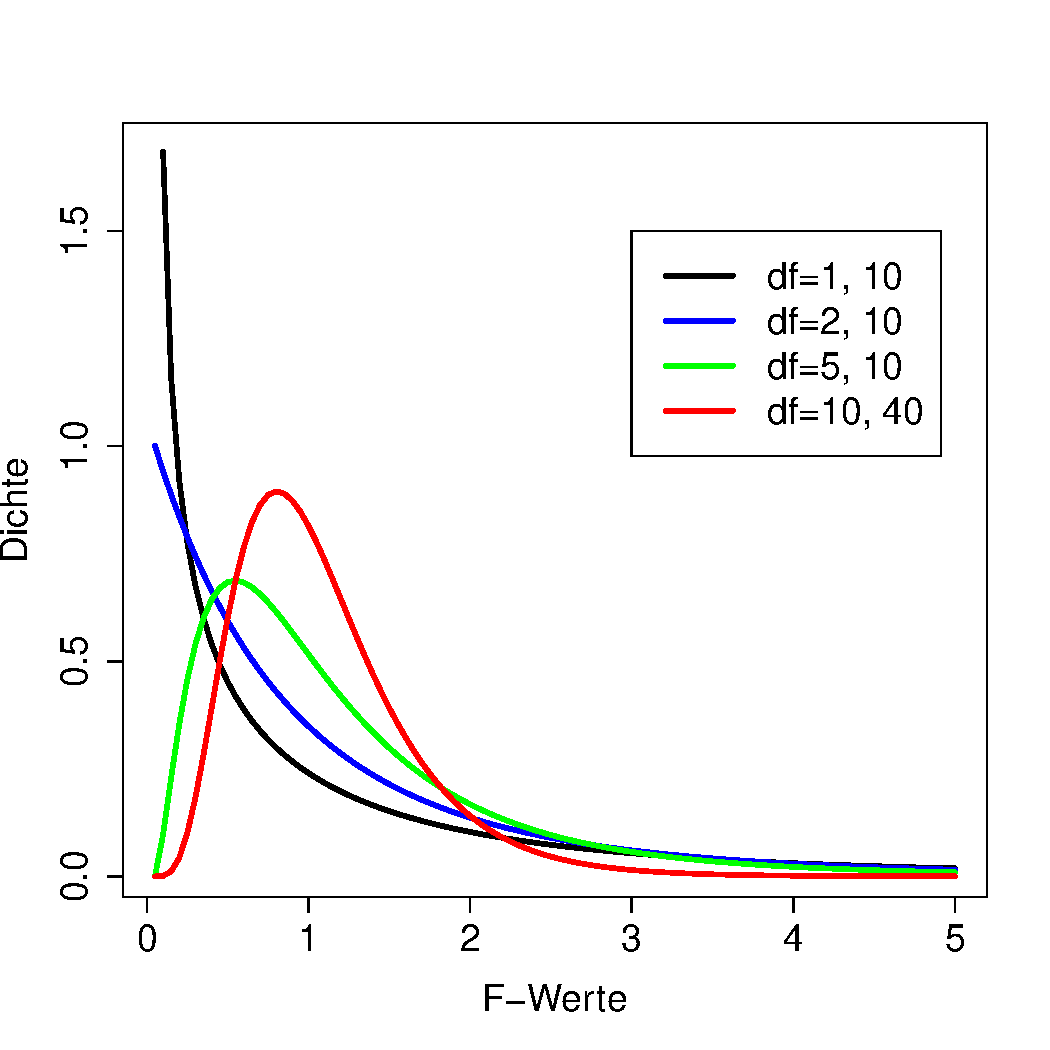
\includegraphics[width=0.3\textwidth]{anova_fdist}
  \end{center}

  \vspace{0.5cm}
  In \texttt{R} für $df_{zwischen}=2$ und $df_{in}=12$ bei sig=0.05:\\
  \texttt{> qf(0.95, 2, 12) $\Rightarrow$ 3.885294}
\end{frame}

\begin{frame}
  {Effektstärke}

  \begin{center}
    \alert{$\eta^2=\frac{SQ_{zwischen}}{SQ_{gesamt}}$}\\[4ex]
    (wieder ein $r^2$-Maß)
  \end{center}
\end{frame}

\begin{frame}
  {Post-Hoc-Tests}
  \begin{itemize}[<+->]
    \item Problem: \alert{Welche Gruppen unterscheiden sich denn nun?}
    \Zeile
    \item Lösung: Post(-Hoc)-Tests, \zB Scheff\'e-Test:
      \begin{itemize}
	\item \alert{paarweise ANOVA}
	\item aber: \alert{$k$} wird gesetzt \alert{wie bei ursprünglicher ANOVA}
	\item dadurch Vermeidung kumulierten Alpha-Fehlers\\
	  (Vorteil ggü.\ paarweisen t-Tests)
	\item weiterer Vorteil: paarweise Post-Tests nur erforderlich,\\
	  wenn \alert{Omnibus-ANOVA} bereits Signifikanz gezeigt hat
	\item und: Generalisierbarkeit zu mehrfaktorieller ANOVA\\
	  (geht mi t-Test nicht)
      \end{itemize}
  \end{itemize}

  \vspace{0.2cm}
  \pause
  \begin{center}
    Bitte ausrechnen für die oben gerechnete ANOVA.
  \end{center}
\end{frame}

\subsection{Zweifaktorielle ANOVA}

\begin{frame}
  {Wozu mehrfaktorielle Designs}

  Oft vermutet man den Einfluss \alert{mehrerer Unabhängiger} auf eine Abhängige.\\
  Beispiel: Satzlängen

  \begin{center}
    \begin{tabular}[h!]{|cc|ccc|}
      \cline{3-5}
      \multicolumn{2}{c|}{} & \multicolumn{3}{c|}{\textbf{Textsorte}} \\
      \multicolumn{2}{c|}{} & \textbf{Fiktion} & \textbf{Zeitung} & \textbf{Wissenschaft} \\
      \hline
      \multirow{2}{*}{\textbf{Jahrhundert}} & \textbf{19} & $x_{11}$ & $x_{12}$ & $x_{13}$ \\
      & \textbf{20} & $x_{21}$ & $x_{22}$ & $x_{23}$ \\
      \hline
    \end{tabular}\\
    \vspace{0.5cm}

    Hier also: $2\cdot3=6$ Gruppen
  \end{center}
\end{frame}

\begin{frame}
  {Ablauf der zweifaktoriellen ANOVA}
  \begin{enumerate}[<+->]
    \item erste ANOVA zwischen Zeilen
    \item zweite ANOVA zwischen Spalten
    \item dritte ANOVA für \alert{Interaktionen} zwischen Zeilen und Spalten
    \Zeile
    \item Interaktion: Ungleichverteilung in Gruppen, die nicht\\
      durch die Spalten- und Zeileneffekte erklärt werden kann
    \Zeile
    \item Alle drei ANOVAs sind \alert{unabhängig} voneinander!
  \end{enumerate}
\end{frame}

\begin{frame}
  {Komponenten der zweifaktoriellen ANOVA}
  \begin{itemize}[<+->]
    \item \alert{Gesamtvarianz} = Varianz zwischen Gruppen + Varianz in den Gruppen
    \Zeile
    \item \alert{Varianz zwischen den Gruppen} =\\
      Haupt-Faktoren-Varianz + \alert{Interaktions-Varianz}
    \Zeile
    \item \alert{Haupt-Faktoren-Varianz} =\\
      Varianz zwischen Faktor A-Gruppen +\\
      Varianz zwischen Faktor B-Gruppen
  \end{itemize}
\end{frame}

\begin{frame}
  {Schritt 1(1): SQ\slash df zwischen den Gruppen}
  \alert{Jede Zelle} der Tabelle ist eine Gruppe.

  \begin{center}
    \alert{$SQ_{zwischen}=\sum\limits_i(\frac{T_i^2}{n_i})-\frac{G^2}{N}$}\\

    \alert{$df_{zwischen}=k-1$} (k = Anzahl der Zellen\slash Gruppen)
  \end{center}
  \vspace{1cm}
  Beachte: \alert{Keine} Änderung verglichen mit einfaktorieller ANOVA!
\end{frame}

\begin{frame}
  {Schritt 1(2): SQ\slash df in den Gruppen}
  \alert{Jede Zelle} der Tabelle ist eine Gruppe.

  \begin{center}
    \alert{$SQ_{in}=\sum SQ(x_i)$}\\

    \alert{$df_{in}=\sum df(x_i)$}
  \end{center}
  \vspace{1cm}
  Beachte: \alert{Keine} Änderung verglichen mit einfaktorieller ANOVA!
\end{frame}

\begin{frame}
  {Schritt 2(2): SQ\slash df für Gruppe A}

  Berechnung nach dem Schema für Zwischen-Gruppen-Varianz

  \begin{center}
    \begin{tabular}[h!]{|cc|ccc||c|}
      \cline{3-5}
      \multicolumn{2}{c|}{} & \multicolumn{3}{c||}{\textbf{Textsorte}} & \multicolumn{1}{c}{}\\
      \multicolumn{2}{c|}{} & \textbf{Fiktion} & \textbf{Zeitung} & \textbf{Wissenschaft} & \multicolumn{1}{c}{}\\
      \hline
      \multirow{2}{*}{\textbf{Jahrhundert}} & \textbf{19} & $x_{11}$ & $x_{12}$ & $x_{13}$ & \alert{$A_1$}\\
      & \textbf{20} & $x_{21}$ & $x_{22}$ & $x_{23}$ & \alert{$A_2$}\\
      \hline
    \end{tabular}\\
    \vspace{0.5cm}

    Auch hier keine wesentliche Änderung:\\
    \alert{$SQ_{A}=\sum\limits_i(\frac{T_{A_i}^2}{n_{A_i}})-\frac{G^2}{N}$}\\
    \alert{$df_{A}=k_A-1$} ($k_A$ = Anzahl der \alert{Zeilen})
  \end{center}
\end{frame}

\begin{frame}
  {Schritt 2(2): SQ\slash df für Gruppe A}

  Berechnung nach dem Schema für Zwischen-Gruppen-Varianz

  \begin{center}
    \begin{tabular}[h!]{|cc|ccc|}
      \cline{3-5}
      \multicolumn{2}{c|}{} & \multicolumn{3}{c|}{\textbf{Textsorte}} \\
      \multicolumn{2}{c|}{} & \textbf{Fiktion} & \textbf{Zeitung} & \textbf{Wissenschaft} \\
      \hline
      \multirow{2}{*}{\textbf{Jahrhundert}} & \textbf{19} & $x_{11}$ & $x_{21}$ & $x_{31}$ \\
      & \textbf{20} & $x_{12}$ & $x_{22}$ & $x_{32}$ \\
      \hline\hline
      \multicolumn{2}{c|}{} & \alert{$B_1$} & \alert{$B_2$} & \alert{$B_3$} \\
      \cline{3-5}
    \end{tabular}\\
    \vspace{0.5cm}

    Auch hier keine Änderung:\\
    \alert{$SQ_{B}=\sum\limits_i(\frac{T_{B_i}^2}{n_{B_i}})-\frac{G^2}{N}$}\\
    \alert{$df_{B}=k_B-1$} ($k_B$ = hier Anzahl der \alert{Spalten})
  \end{center}
\end{frame}

\begin{frame}
  {Schritt 2(3): SQ\slash df für Interaktion $A\times B$}
  Die Varianz, die auf Kosten der Interaktion geht, ist\\
  \alert{die Zwischen-Gruppen-Varianz ohne die Einzelfaktor-Varianz}.\\

  \vspace{0.5cm}
  \begin{center}
    $SQ_{A\times B}=SQ_{zwischen}-SQ_A-SQ_B$\\
    $df_{A\times B}=df_{zwischen}-df_A-df_B$
  \end{center}
\end{frame}

\begin{frame}
  {Alle drei F-Werte ausrechnen}
  Die \alert{zwei}faktorielle ANOVA\\
  erfordert wie gesagt \alert{drei} Einzel-ANOVAs.\\

  \begin{center}
    $F_A=\frac{\frac{SQ_A}{df_A}}{\ \ \ \frac{SQ_{zwischen}}{df_{zwischen}}\ \ \ }=\frac{s^2_A}{s^2_{zwischen}}$\\[3ex]
    $F_B=\frac{\frac{SQ_A}{df_B}}{\ \ \ \frac{SQ_{zwischen}}{df_{zwischen}}\ \ \ }=\frac{s^2_B}{s^2_{zwischen}}$\\[3ex]
    $F_{A\times B}=\frac{\frac{SQ_{A\times B}}{df_{A\times B}}}{\ \ \ \frac{SQ_{zwischen}}{df_{zwischen}}\ \ \ }=\frac{s^2_{A\times B}}{s^2_{zwischen}}$\\
  \end{center}
\end{frame}

\begin{frame}
  {Effektstärken}
  Entsprechend sind \alert{drei} $\eta^2$ auszurechnen:\\

  \vspace{0.5cm}
  \begin{center}
    $\eta^2_A=\frac{SQ_A}{SQ_{gesamt} - SQ_B - SQ_{A\times B}}$ \\[3ex]
    $\eta^2_B=\frac{SQ_B}{SQ_{gesamt} - SQ_A - SQ_{A\times B}}$ \\[3ex]
    $\eta^2_{A\times B}=\frac{SQ_{A\times B}}{SQ_{gesamt} - SQ_A - SQ_B}$ \\
  \end{center}

  Wir fragen jeweils, welchen Anteil an der Varianz,\\
  die die anderen beiden Faktoren \alert{nicht} erklären,\\
  der jeweilige dritte Faktor hat.
\end{frame}

\begin{frame}
  {Das jetzt alles zusammen}
  Bitte vollständige zweifaktorielle ANOVA\\
  bei sig=0.05 und sig=0.01 rechnen:\\

  \begin{center}
    \begin{tabular}[h!]{|c||c|c|c|}
      \hline
      & \textbf{B1} & \textbf{B2} & \textbf{B3} \\
      \hline
      \hline
      \textbf{A1} & $1, 3, 1, 4$ & $4, 3, 3, 6$ & $8, 6, 8, 10$ \\
      \hline
      \textbf{A2} & $8, 6, 6, 8$ & $1, 6, 8, 1$ & $1, 4, 1, 4$ \\
      \hline
    \end{tabular}
  \end{center}
\end{frame}

  \let\subsection\section\let\section\woopsi

  \section{Nichtparametrische Verfahren}
  \let\woopsi\section\let\section\subsection\let\subsection\subsubsection
  \section[Zähldaten]{Testverfahren für Zähldaten}

\begin{frame}
  {Übersicht}
  \begin{itemize}[<+->]
%    \item Einführung in Verfahren mit \alert{Test-Werten}
    \item Unterschiede in Zähldaten 
    \item Signifikanz und Effektstärke
    \item Unterschiede bei Ja\slash Nein-Experimenten
  \end{itemize}
\end{frame}

\begin{frame}
  {Literatur}
  \begin{itemize}
    \item \cite{GravetterWallnau2007}
    \item \cite{BortzLienert2008}
  \end{itemize}
\end{frame}

%\subsection{Nichtparametrisch}
%
%\begin{frame}
%  {Nicht-parametrische Tests}
%  \begin{itemize}[<+->]
%    \item Erforderliche \alert{Verteilungsparameter} für Variablen in vielen Tests:
%      \begin{itemize}[<+->]
%	\item normalverteilt
%	\item Varianzhomogenität der Gruppen
%      \end{itemize}
%    \item Vortests auf solche \alert{Verteilungsparameter}:
%      \begin{itemize}[<+->]
%	\item Normalität: \zB Shapiro-Wilk-Test
%	\item Varianzhomogenität: \zB Bartlett-Test
%      \end{itemize}
%    \item Nichtparametrische Tests: keine solchen Voraussetzungen
%    \item Korpusstudien: oft \alert{Zähldaten}, weniger oft Intervalldaten.
%  \end{itemize}
%\end{frame}

\subsection{Vierfelder-Unterschiedstest}

\begin{frame}{Kreuztabelle}
  Beobachtungen von zwei \alert{kategorialen Variablen}.\\
  Auxiliarwahl beim Perfekt: haben, sein\\
  Herkunft des Belegs: nord, sued\\

\begin{figure}[h]
  \centering
  \begin{tabular}{ccc}
    \textbf{Fall} & \textbf{Aux} & \textbf{Region} \\
          1       & haben        & nord   \\
          2       & haben        & nord   \\
          3       & sein         & nord  \\
          4       & sein         & sued  \\
          5       & sein         & sued   \\
          6       & haben        & nord   \\
          7       & haben        & sued   \\
          8       & haben        & sued  \\             
  \end{tabular}
  \onslide<2->{
    \begin{tabular}{|c|c|c|}
      \hline
      & \multicolumn{2}{c|}{\textbf{Aux}}\\
      \hline
      \textbf{Region}      &  haben & sein\\
      \hline
	nord   &   3     &   1\\
      \hline
	sued   &    2    &   2\\
      \hline
    \end{tabular}}
\end{figure}
\end{frame}


\begin{frame}{Kreuztabelle mit Randsummen}

  Spaltensumme für Spalte $i$: \alert{$\sum\limits_{k}x_{ik}$}\\
  Zeilensumme für Zeile $j$: \alert{$\sum\limits_{k}x_{kj}$}\\

\begin{figure}[h]
  \centering
  \begin{tabular}{|c|c|c||c|}
    \hline
    &  haben & sein & Zeilensummen\\
    \hline
    nord   &   3     &  1   & \onslide<2->{\gruen{4}} \\
    \hline
    sued   &    2   &   2   &  \onslide<3->{\gruen{4}}\\
    \hline
    \hline
    Spaltensummen &   \onslide<4->{\rot{5}}   &  \onslide<5->{\rot{3}} & \onslide<6->{\textbf{8}}\\
    \hline
  \end{tabular}
\end{figure}
\end{frame}


\begin{frame}{Beobachtete vs.\ erwartete Häufigkeiten}

  n=100\\
  50 mal \textit{haben}, 50 mal \textit{sein} (= \alert{Spaltensummen})\\ 
  50 mal Norden, 50 mal Süden (= \alert{Zeilensummen})\\

  \begin{itemize}
    \item<2-> erwartete Häufigkeiten unter Annahme der \Null\\
    = kein Zusammenhang zwischen Hilfsverb und Region?
  \end{itemize}

  \begin{figure}[h]
  \centering
  \begin{tabular}{|c|c|c||c|}
    \hline
	  &  haben & sein & Zeilensummen\\
    \hline
      nord   &  \onslide<3>{25}      &  \onslide<3>{25}    & \onslide<1->{\gruen{50}} \\
    \hline
      sued   &   \onslide<3>{25}      &  \onslide<3>{25}    &  \onslide<1->{\gruen{50}}\\
    \hline
    \hline
     Spaltensummen &  \onslide<1->{\rot{50}}   & \onslide<1->{\rot{50}}  & \textbf{100}\\
    \hline
  \end{tabular}
  \end{figure}
\end{frame}


\begin{frame}{Beobachtete vs.\ erwartete Häufigkeiten}
    n=100\\
    50 mal \textit{haben}, 50 mal \textit{sein} (= \alert{Spaltensummen})\\
    30 mal Norden, 70 mal Süden (= \alert{Zeilensummen})\\

  \begin{itemize}
    \item<1-> erwartete Häufigkeiten unter Annahme der \Null?
  \end{itemize}

  \begin{figure}[h]
    \centering
    \begin{tabular}{|c|c|c||c|}
  \hline
	&  haben & sein & Zeilensummen\\
  \hline
    nord   &  \onslide<6->{15}      &  \onslide<7->{15}    & \onslide<2->{\gruen{30}} \\
  \hline
    sued   &   \onslide<8->{35}      &  \onslide<9->{35}    &  \onslide<3->{\gruen{70}}\\
  \hline
  \hline
   Spaltensummen &  \onslide<4->{\rot{50}}   & \onslide<5->{\rot{50}}  & \textbf{100}\\
  \hline
    \end{tabular}
  \end{figure}
\end{frame}


\begin{frame}
  {Beobachtete vs.\ erwartete Häufigkeiten}
  \vspace{-1cm}
  n=100\\
  30 mal Norden, 70 mal Süden\\
  40 mal \textit{haben}, 60 mal \textit{sein}\\

  \begin{figure}[h]
  \centering
    \begin{tabular}{|c|c|c||c|}
      \hline
      &  haben & sein & Zeilensummen\\
      \hline
      nord   &  \onslide<2->{12}      &  \onslide<3->{18}    & \onslide<1->{\gruen{30}} \\
      \hline
      sued   &   \onslide<4->{28}      &  \onslide<5->{42}    &  \onslide<1->{\gruen{70}}\\
      \hline
      \hline
      Spaltensummen &  \onslide<1->{\rot{40}}   & \onslide<1->{\rot{60}}  & \textbf{100}\\
      \hline
    \end{tabular}
  \end{figure}

  \begin{center}
    Allgemein: erwartete Häufigkeit für Zellen: $\frac{Spaltensumme \cdot Zeilensumme}{n}$\\[2ex]
    bzw.: \alert{$EH(x_{ij})=\frac{\sum\limits_{k}x_{ik}\cdot\sum\limits_{k}x_{kj}}{n}$}
  \end{center}
\end{frame}


\begin{frame}
  {Beobachtete vs.\ erwartete Häufigkeiten}
beobachtete Häufigkeiten für eine DeReKo-Stichprobe (\textit{geschwebt}):

  \begin{figure}[h]
    \centering
    \begin{tabular}{|c|c|c||c|}
  \hline
	&  haben & sein & Zeilensummen\\
  \hline
    nord   &  27      & 33    & \onslide<1->{\gruen{60}} \\
  \hline
    sued   &   3      & 34    &  \onslide<1->{\gruen{37}}\\
  \hline
  \hline
   Spaltensummen &   \onslide<1->{\rot{30}}   &  \onslide<1->{\rot{67}} & \textbf{97}\\
  \hline
    \end{tabular}
  \end{figure}
  \pause

  erwartete Häufigkeiten:
  \begin{figure}[h]
    \centering
    \begin{tabular}{|c|c|c||c|}
  \hline
	&  haben & sein & Zeilensummen\\
  \hline
    nord   & \visible<3->{18.56}  & \visible<3->{41.44} & \onslide<1->{\gruen{60}} \\
  \hline
    sued   & \visible<3->{11.44}  & \visible<3->{25.56} &  \onslide<1->{\gruen{37}}\\
  \hline
  \hline
   Spaltensummen &   \onslide<1->{\rot{30}}   &  \onslide<1->{\rot{67}} & \textbf{97}\\
  \hline
    \end{tabular}
  \end{figure}
\end{frame}


\begin{frame}{Problem}

  \begin{itemize}[<+->]
  \item Beobachtete und erwartete Häufigkeit weichen ab.
  \item \Null: kein Zusammenhang zwischen Region und Aux.
  \item Ab wann ist der Unterschied "`signifikant"'?
    \vspace{\baselineskip}
  \item Ein gemessener Unterschied ist \alert{siginifikant}, wenn er angesichts der Stichprobengröße groß genug ist, dass wir das im Experiment gefundene Ergenbis nur sehr selten (typischwerweise in unter 5\% der Fälle) erwarten würden, wenn er gar nicht bestünde. 
    \vspace{\baselineskip}
  \item Diese 5\% (als \alert{Anteil} 0.05) sind das \alert{Signifikanzniveau}.
  \item In Fishers Philosophie abgekürzt \Sig, nicht wie oft zu lesen "`$\alpha$-Niveau"'.
\end{itemize}
  
\end{frame}


\begin{frame}{$\chi^2$-Unterschiedstest}
  \begin{figure}[h]
    \centering
    \begin{tabular}{|c|c|c|}
  \multicolumn{3}{c}{beobachtet:}\\
  \hline
	&  haben & sein\\
  \hline
    nord   &  27      & 33 \\
  \hline
    sued   &   3      & 34 \\
  \hline
    \end{tabular}~~~
    \begin{tabular}{|c|c|c|}
  \multicolumn{3}{c}{erwartet:}\\
  \hline
	&  haben & sein\\
  \hline
    nord   &  18.56      & 41.44 \\
  \hline
    sued   &  11.44     & 25.56 \\
  \hline
    \end{tabular}
  \end{figure}
\pause
  \begin{center}
    $\chi^2 = \sum \frac{(beobachtet - erwartet)^2}{erwartet}$\\[3ex]
    \pause
    bzw.: \alert{$\chi^2=\sum\limits_{ij}\frac{(x_{ij}-EH(x_{ij}))^2}{EH(x_{ij})}$}
  \end{center}
\end{frame}


\begin{frame}{Berechnung des $\chi^2$-Werts}
  $\chi^2 = \sum \frac{(beobachtet - erwartet)^2}{erwartet}$\\
  \vspace{1cm}

  \begin{center}
    \begin{tabular}{|c|c|c|}
      \multicolumn{3}{c}{beobachtet:}\\
      \hline
      &  haben & sein\\
      \hline
      nord   &  {\gruen{27}}      & {\gruen{33}} \\
      \hline
      sued   &   {\gruen{3}}      & {\gruen{34}} \\
      \hline
      \end{tabular}
      \ \ \ 
      \begin{tabular}{|c|c|c|}
      \multicolumn{3}{c}{erwartet:}\\
      \hline
	    &  haben & sein\\
      \hline
	nord   &  {\gruen{18.56}}      & {\gruen{41.44}} \\
      \hline
	sued   &  {\gruen{11.44}}      & {\gruen{25.56}} \\
      \hline
    \end{tabular}
  \end{center}

  \begin{tabular}{lc@{~}c@{~}c@{~}c@{~}c}
    \visible<2->{$\chi^2$ =} & \visible<2->{\(\frac{(27-18.56)^2}{18.56}\)} & \visible<3->{+~\( \frac{(33-41.44)^2}{41.44}\)} &\visible<4->{+~\( \frac{(3-11.44)^2}{11.44}\)} & \visible<5->{+~\( \frac{(34-25.56)^2}{25.56}\)}&\\
    \visible<6->{$\chi^2$ =} & \visible<6->{3.84} &  \visible<6->{+ ~~~1.72} & \visible<6->{+ ~~~6.23} & \visible<6->{+ ~~~2.79} &  \visible<6->{= ~~\onslide<1->{\alert{14.58}}}
  \end{tabular}
\end{frame}



\begin{frame}
  {Die $\chi^2$-Verteilung}
  Die $\chi^2$-Verteilung für Stichproben\\
  aus Grundgesamtheiten ohne Zusammenhang:
  \begin{center}
    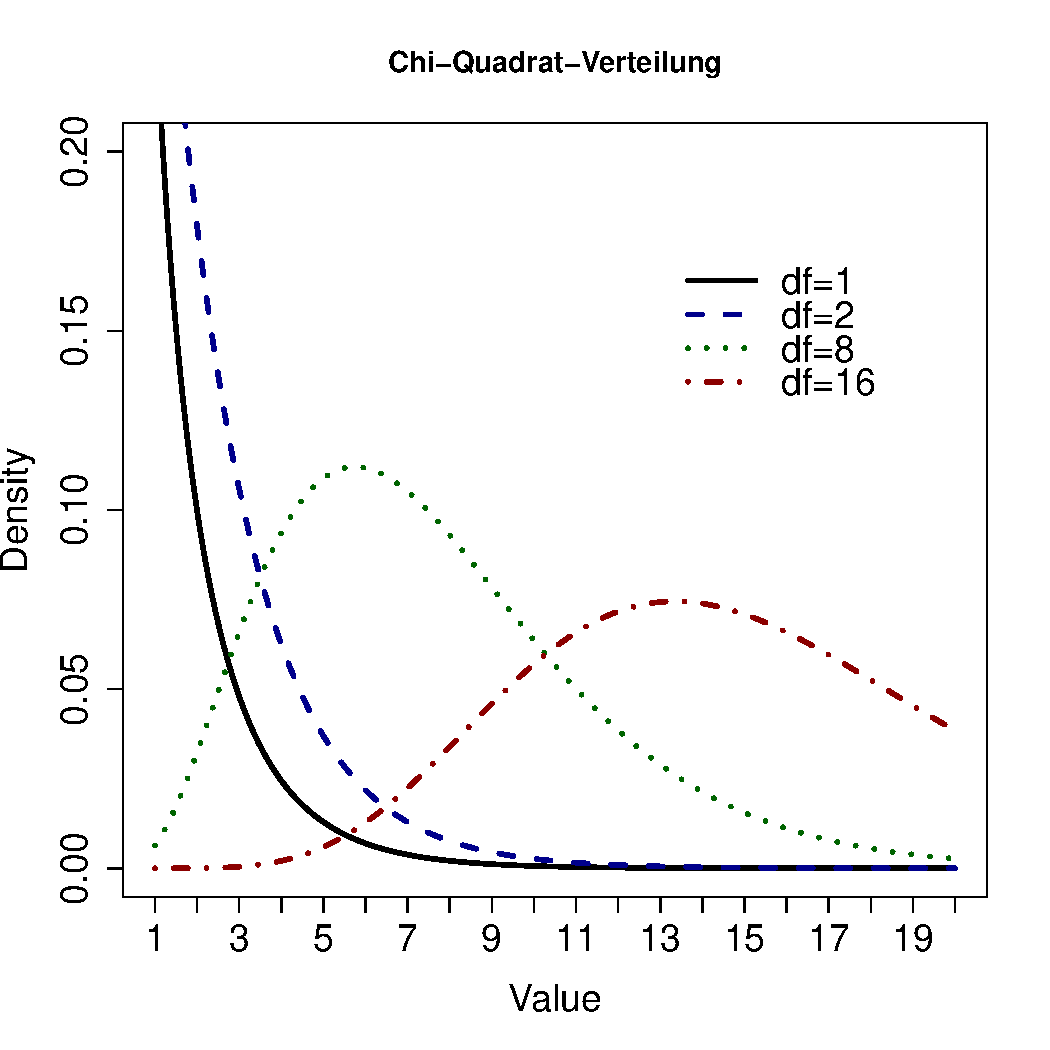
\includegraphics[width=5cm]{graphics/chisq}
  \end{center}
\end{frame}

\begin{frame}
  {Freiheitsgrad?}
  Was sind \alert{"`Freiheitsgrade"'} oder \textit{degrees of freedom (df)}?

  \begin{itemize}[<+->]
    \item Das kommt später noch ausführlicher.
    \item Für n-Felder-Tests: \alert{(Zeilenzahl$-1$)$\cdot$(Spaltenzahl$-1$)}
    \item Bei Vierfelder-Test also: $df=1$
  \end{itemize}
\end{frame}

\begin{frame}{Die $\chi^2$-Verteilung II}
  \begin{itemize}[<+->]
    \item Wahrscheinlichkeit eines bestimmten $\chi^2$-Werts unter Annahme der \Null?\\
      \alert{VOR dem Experiment! Nach dem Experiment ist die Wahrscheinlichkeit\\
      des gemessenen p-Werts immer 1.}
      \vspace{\baselineskip}
    \item In Fishers Philosophie Entscheidung nach \alert{Signifikanzniveau} (\Sig):\\
      \alert{Der $\chi^2$-Wert muss in den extremen \Sig-Anteilen liegen,\\
      um die \Null\ zu \Sig\ zurückzuweisen.}
  \end{itemize}
  \pause
  \begin{center}
    In \texttt{R} ähnlich wie bei Normalverteilung:\\
    \texttt{> qchisq(0.95, df=1) $\Rightarrow$ \texttt{3.84}}
  \end{center}
  \pause
  \begin{itemize}
    \item Also ist für $\chi^2=14.58$ auf jeden Fall $p<0.05$ (weil $14.58>3.84$).
  \end{itemize}
\end{frame}


\begin{frame}
  {Mehr oder weniger signifikant?}
  \begin{itemize}[<+->]
    \item Oft liest man etwas von "`$\alpha$-Niveaus"' wie:
      \begin{itemize}[<+->]
	\item 5\% ("`signifikant"')
	\item 1\%
	\item 0.1\% ("`hochsignifikant"')
      \end{itemize}
    \item Diese Niveaus entsprechen einem falsch interpretierten \Sig.
    \item Die Idee von "`mehr oder weniger signifikant"' ist \alert{kompletter Schwachsinn}.
    \item Entweder ist das gesetzte Niveau akzeptabel,\\
      und dann bringt ein kleineres $p$ aber auch nicht mehr.
    \item Oder es müsste eigtl.\ ein strengeres \Sig-Niveau gewählt werden,\\
      und dann ist $p<0.05$ schlicht nicht ausreichend (s.\ Fishers \alert{Sensitivität}).
    \item Die Entscheidung für ein bestimmtes \Sig-Niveau muss\\
      auf Basis konzeptueller\slash inhaltlicher Gründe gefällt werden.
    \item \alert{EIN signifikantes Testergebnis alleine sagt nicht viel aus!!!}
  \end{itemize}
\end{frame}




\begin{frame}{Voraussetzungen für $\chi^2$-Tests}
  \begin{enumerate}[<+->]
    \item Die Beoabachtungen sind voneinander unabhängig.
    \item In jeder Zelle ist die erwartete Häufigkeit mindestens 5.
    \item Keine Beschränkung auf vier Felder!
  \end{enumerate}
\end{frame}

\begin{frame}
  {In \texttt{R}}
  Mit einer Matrix \texttt{my.matrix}:\\
  \texttt{> chisq.test(my.matrix)}\\
  \vspace{0.5cm}
  
  Eingabe einer einfachen Vierfeldermatrix:\\
  \texttt{> my.matrix <- matrix(c(27,33,3,34), 2, 2, byrow=TRUE)}\\
  \vspace{0.5cm}
  
  Ausgeben der erwarteten Häufigkeiten:\\
  \texttt{> chisq.test(my.matrix)\$expected}\\

  \end{frame}

  \subsection[Fisher-Exakt]{Fisher-Exakt-Test}

\begin{frame}
  {Wann und wie Fisher-Exakt?}
  \alert{Der Fisher-Exakt-Test ist eine Alternative zum $\chi^2$-Test.}\\[3ex]

  \begin{itemize}[<+->]
    \item exakter Test: direkte Berechnung der Wahrscheinlichkeit
    \item \alert{keine} allgemein bessere Alternative zu $\chi^2$
    \item robuster bei sehr kleinen Stichproben
    \item \alert{aber nur für feststehende Randsummen geeignet!}
    \item ohne feste Randsummen: \alert{Barnards Test}
  \end{itemize}
  \vspace{0.5cm}
  
  \visible<4->{
    Fisher-Exakt in \texttt{R}:\\
    \vspace{0.3cm}
    \texttt{> fisher.test(my.matrix)}\\
    \texttt{> fisher.test(my.vector.1, my.vector.2)}
  }
\end{frame}

%\subsection[$\chi^2$ (Anpassung)]{$\chi^2$-Anpassungstest}
%
%\begin{frame}
%  {Situation für Anpassungstests}
%  \begin{itemize}[<+->]
%    \item bei \alert{bekannter Verteilung} können beobachtete Verteilungen\\
%      auf Übereinstimmung (Fit) damit getestet werden.
%    \item \alert{Die Nullhypothese ist bei allen Anpassungstests der Fit!}
%    \item \alert{Erreichen des $\alpha$-Niveaus} = Zurückweisung der Nullhypothese:\\
%      \alert{Stichprobe (wahrscheinlich) nicht\slash nicht zufällig der GG entnommen.}
%    \item typischer Einsatz: Anpassungen an theoretische Verteilungen
%  \end{itemize}
%\end{frame}
%
%\begin{frame}
%  {Beispiel $\chi^2$-Anpassungstest}
%  \begin{itemize}[<+->]
%    \item Bsp.: Wir kennen die Verteilung von pronominalen\\
%      und nicht-pronominalen Subjekten im gesamten Korpus und\dots
%    \item \dots haben an einer Stichprobe die Verteilung bei \textit{anhören} gemessen.
%  \end{itemize}
%  \pause
%  \begin{center}
%    \begin{tabular}{|c|c|c|c|}
%      \hline
%       & pronominal & nicht-pronominal & $\Sigma$ \\
%      \hline\hline
%      Verteilung & $0.39$ & $0.61$ & $1$ \\
%      \hline\hline
%      Stichprobe & $108$ & $126$ & $234$ \\
%      \hline
%      erwartet & $91.26$  & $142.74$  & $234$ \\
%      \hline
%    \end{tabular}
%  \end{center}
%  \pause
%  Die Berechnung erfolgt nach bekanntem Schema.
%\end{frame}
%
%\begin{frame}
%  {In \texttt{R}}
%  Vektor mit Verteilungs-Wahrscheinlichkeiten:\\
%  \texttt{> my.prob <- c(0.39, 0.61)}
%  \vspace{.5cm}
%
%  Vektor mit Messungen:\\
%  \texttt{> my.data <- c(108, 126)}
%  \vspace{.5cm}
%
%  Testen:\\
%  \texttt{> my.chi2 <- chisq.test(my.data, p=my.prob); my.chi2}
%\end{frame}


\subsection[Effektstärke]{Effektstärke: Cramérs $v$}

\begin{frame}{Effektstärke}

  Der $\chi^2$-Wert sagt nichts über die \alert{Stärke eines Zusammenhangs}!\\
  \onslide<2->{Bei höheren absoluten Frequenzen wird auch der $\chi^2$-Wert größer.}

  \begin{figure}[h]
    \centering
    \begin{tabular}{|c|c|c|}
      \hline
      &  haben & sein\\
      \hline
      nord   &  27      & 33 \\
      \hline
	sued   &   3      & 34 \\
      \hline
    \end{tabular}~$\chi^2$ = \onslide<4->{\alert{12,89}}~\visible<6->{
    \begin{tabular}{|c|c|c|}
      \hline
	    &  haben & sein\\
      \hline
	nord   &  27.84\% & 34.02\% \\
      \hline
	sued   &  3.09\%     & 35.05\% \\
      \hline
    \end{tabular}
    }
  \end{figure}

  \begin{figure}[h]
    \centering
    \begin{tabular}{|c|c|c|}
      \hline
	    &  haben & sein\\
      \hline
	nord   &  54      & 66 \\
      \hline
	sued   &  6     & 68 \\
      \hline
      \end{tabular}~$\chi^2$ = \onslide<5->{\alert{27,46}}~\visible<7->{
      \begin{tabular}{|c|c|c|}
      \hline
	    &  haben & sein\\
      \hline
	nord   &  27.84\%      & 34.02\% \\
      \hline
	sued   &   3.09\%      & 35.05\% \\
      \hline
    \end{tabular}
  }
  \end{figure}
\end{frame}


\begin{frame}{Effektstärke II}
  Pearsons $\phi$: Maß für die Stärke des Zusammenhangs in 2$\times$2-Tabellen
    
  \begin{figure}
    \centering
    \alert{$\phi = \sqrt{\frac{\chi^2}{n}}$}
  \end{figure}

  \visible<2->{$\phi$ ist eine Zahl zwischen 0 und 1:\\
  Je größer, desto stärker der Zusammenhang zwischen den Variablen.}

  \visible<3->{
  \begin{figure}
  \centering
  Beispiel: \(\phi = \sqrt{\frac{\chi^2}{n}} = \sqrt{\frac{12.89}{97}} = \onslide<1->{\alert{0.3648}\)}}
  \end{figure}
\end{frame}


\begin{frame}
  {Cramérs $v$}

  Cramérs $v$ für $n\times n$-Tabellen mit $n>2$ oder $m>2$

  \begin{center}
    \alert{$v=\sqrt{\frac{\frac{\chi^2}{n}}{min(s-1,z-1)}}$}\\
    mit: $s$ die Spaltenzahl und $z$ die Zeilenzahl
  \end{center}

  \vspace{1cm}
  \footnotesize
  Beachte: für $2\times2$-Tabellen: $s-1=1$ und $z-1=1$,\\[2ex]
  also $min(s-1,z-1)=1$\\[1ex]
  daher: $v=\sqrt{\frac{\ \ \frac{\chi^2}{n}\ \ }{1}}=\sqrt{\frac{\chi^2}{n}}=\phi$

\end{frame}


\begin{frame}
  {In \texttt{R}}
  Speichern des Test-Objekts:\\
  \texttt{> my.chi2.test <- chisq.test(my.matrix)}\\
  \vspace{0.5cm}
  
  Speichern des $\chi^2$-Werts mit:\\
  \texttt{> my.chi2.value <- as.numeric(my.chi2.test\$statistic})\\
  \vspace{0.5cm}
  
  Speichern von $n$:\\
  \texttt{> my.n <- sum(my.matrix)}\\
  \vspace{0.5cm}

  Also Effektstärke (mit Ausgabe):\\
  \texttt{> my.phi <- sqrt( my.chi2.value / my.n ); my.phi}
\end{frame}

\subsection[Chancenverhältnis]{Chancenverhältnis}

\begin{frame}
  {Chance (odds)}
  \begin{itemize}[<+->]
    \item Die \alert{Chance (odds)} $o$ setzt die Wahrscheinlichkeit $p$ eines Ereignisses $E$\\
      in Relation zur Gegenwahrscheinlichkeit:
  \end{itemize}
  \pause
   \begin{center}
     \alert{$o(E)=\frac{p(E)}{1-p(E)}$}\\[2ex]
     \pause
     und damit\\[2ex]
     \pause
     \alert{$p(E)=\frac{o(E)}{1+o(E)}$}
  \end{center}
  \pause
  \begin{itemize}[<+->]
    \item Ein Ereignis ist in Korpusstudien i.\,d.\,R.\\\
      das Auftreten einer \alert{Variablenausprägung}.
    \item Die Information in den Maßen Wahrscheinlichkeit und Chance\\
      ist dieselbe (s. Umrechenbarkeit ineinander).
  \end{itemize}
\end{frame}

\begin{frame}
  {Chance und Wahrscheinlichkeit und Zähldaten}
  \vspace{-1cm}
      \begin{center}
	\begin{tabular}{|c|c|}
	      \hline
	      \textbf{Aux} & \textbf{Anzahl} \\
	      \hline
	      haben   &  27   \\
	      \hline
	      sein   &  33   \\
	      \hline
	    \end{tabular}\\
      \end{center}
      \pause
      $p(haben)=\frac{27}{27+33}=\frac{27}{60}=0.45$ (Wahrscheinlichkeit)\\[2ex]
      \pause
      $1-p(haben)=p(\neg haben)=\frac{33}{27+33}=\frac{33}{60}=0.55$ (\alert{Gegenwahrscheinlichkeit})\\[2ex]
      \pause
      Beachte: $p(haben)+p(\neg haben)=1$\\[2ex]
      \pause
      \alert{$o(haben)=\frac{\ \frac{27}{60}\ }{\frac{33}{60}}=\frac{27}{60}\cdot\frac{60}{33}=\frac{27}{33}=0.82$}\\[2ex]
      \pause
      allgmein: \alert{$p(E)=\frac{Anzahl(E)}{Anzahl(E)+Anzahl(\neg E)}$} und \alert{$o(E)=\frac{Anzahl(E)}{Anzahl(\neg E)}$}\\[2ex]
\end{frame}

\begin{frame}
  {Chancenverhältnis (odds ratio)}
  \begin{itemize}
    \item Das \alert{Chancenverhältnis (odds ratio)} gibt das Verhältnis an, wie sich die Chancen einer Variablenausprägung $E$ unter Bedingung $A$ -- also $o(E|A)$ -- und unter Bedingung $B$ -- also $o(E|B)$ -- zueinander Verhalten:
  \end{itemize}
  \begin{center}
    \alert{$r(E|A, E|B)=\frac{o(E|A)}{o(E|B)}$}
  \end{center}
\end{frame}

\begin{frame}
  {Beispiel zum Chancenverhältnis (1)}
  \begin{itemize}
    \item Wir haben Texte aus Süddeutschland und Norddeutschland auf das Auftreten des Perfektauxiliars \textit{haben} und \textit{sein} bei bestimmten Verben untersucht.
    \item Die Kreuztabelle:
      \begin{center}
	\begin{tabular}{|c|c|c|}
	      \hline
	      &  nord & sued \\
	      \hline
	      haben   &  27      & 3   \\
	      \hline
	      sein   &  33      & 34  \\
	      \hline
	\end{tabular}
      \end{center}
  \end{itemize}
\end{frame}

\begin{frame}
  {Beispiel zum Chancenverhältnis (2)}
    \begin{center}
      \scalebox{0.7}{
	\begin{tabular}{|c|c|c|}
	      \hline
	      &  nord & sued \\
	      \hline
	      haben   &  27      & 3   \\
	      \hline
	      sein   &  33      & 34  \\
	      \hline
	\end{tabular}
      }
    \end{center}
    \begin{itemize}
      \item $o(haben|nord)=\onslide<2->{\frac{27}{33}=0.82$}
      \item $o(haben|sued)=\onslide<3->{\frac{3}{34}=0.09$}
	\pause\pause\pause
      \item Verhältnis zwischen den Chancen: \onslide<5->{$or=\frac{0.82}{0.09} = 9.11$}
	\pause\pause
      \item D.\,h.\ die Chance von \textit{haben} ist 9.11 mal größer, wenn die Region \textit{nord} ist.
	\pause
      \item Ersatz für Effektstärke bei Fisher-Test
    \end{itemize}
\end{frame}

%\subsection[PRE]{Proportionale Fehlerreduktion (PRE)}
%
%\begin{frame}
%  {Erwarteter Vorhersagefehler bei einer Variable}
%  \begin{itemize}[<+->]
%    \item Bei der Messung einer Variablen finden wir auch automatisch\\
%      die erwartete Trefferquote für Vorhersagen.
%    \item (Fiktive) Beobachtungsdaten für die Vorhersage\\
%      des Perfektauxiliars bei \textit{gegangen}:
%  \end{itemize}
%  \visible<2->{
%  \begin{center}
%    \begin{tabular}{|c|c|}
%	  \hline
%	  \textbf{Aux} & \textbf{Anzahl} \\
%	  \hline
%	  haben   &  51 \\
%	  \hline
%	  sein   &  56 \\
%	  \hline
%    \end{tabular}
%  \end{center}
%  }
%  \pause
%  \begin{itemize}[<+->]
%    \item Man würde auf Basis dieses Wissens immer \textit{sein} vorhersagen, weil\\
%      (geschätzt an Stichprobe) \alert{$p(sein)>p(haben)$}.
%    \item Der Anteil \alert{korrekter Vorhersagen} ist \visible<7->{$p(sein)=\frac{56}{(51+56)}=0.52$}
%    \item Der erwartete \alert{Fehler} ist \visible<9->{$p(\neg sein)=\frac{51}{(51+56)}=0.48$}
%  \end{itemize}
%\end{frame}
%
%\begin{frame}
%  {Reduktion des Fehlers durch Variablenabhängigkeit}
%  Wir haben aber (fiktiv) die Variable \textit{Region} auch für \textit{gegangen} erfasst:
%    \begin{center}
%      \scalebox{0.7}{
%	\begin{tabular}{|c|c|c|}
%	      \hline
%	      		&  nord & sued \\
%	      \hline
%	      haben   &  \alert{48}      & 3   \\
%	      \hline
%	      sein   &  17      & \alert{39}  \\
%	      \hline
%	\end{tabular}
%      }
%    \end{center}
%    \pause
%    \begin{itemize}
%      \item Bei Kenntnis der Variable \textit{Region} würde man nun:
%	\begin{itemize}
%	  \item bei \textit{Region=nord}\dots \visible<4->{\textit{haben} vorhersagen}
%	  \item bei \textit{Region=sued}\dots \visible<5->{\textit{sein} vorhersagen}
%	\end{itemize}
%      \pause\pause\pause\pause
%      \item Weil der \alert{Modus} der Verteilungen für \textit{Aux=haben} bei \textit{Region=nord}\\
%	und für \textit{Aux=sein} bei \textit{Region=sued} liegt\\
%	spricht man von der jeweiligen \alert{modalen Kategorie}.
%    \end{itemize}
%\end{frame}
%
%\begin{frame}
%  {Goodman \& Kruskal's $\lambda$}
%    \begin{center}
%      \scalebox{0.7}{
%	\begin{tabular}{|c|c|c||c|}
%	      \hline
%	      		&  nord & sued & $\Sigma$\\
%	      \hline
%	      haben   &  48      & 3  & 51  \\
%	      \hline
%	      sein   &  17      & 39 &  56 \\
%	      \hline
%	      \hline
%	      $\Sigma$ &  65   &  42   &  107  \\
%	      \hline
%	\end{tabular}
%      }
%    \end{center}
%    \pause
%    \begin{itemize}[<+->]
%      \item Die Summe der \alert{modalen Kategorien M} zeilenweise:
%	\begin{center}
%	  $\sum\limits_iM_i=48+39=87$ 
%	\end{center}
%      \item Das Maximum und die Summe der \alert{Zeilensummen Z}:
%	\begin{center}
%	  $max(Z)=56$\hspace{3cm}$\sum\limits_iZ_i=107$
%	\end{center}
%      \item Die \alert{$\lambda$-Fehlerreduktion} ($i$-Indexe weggelassen):
%	\begin{center}
%	  $\lambda=\frac{Fehlerverbesserung\ durch\ Zusatzinfo}{Fehler\ ohne\ Zusatzinfo}=\frac{(\sum M)-max(Z)}{(\sum Z)-max(Z)}=\frac{87-56}{107-56}=\frac{31}{51}=0.61$
%	\end{center}
%    \end{itemize}
%\end{frame}
%
%\begin{frame}
%  {Intuitivere Erklärung}
%  \begin{center}
%      \scalebox{0.7}{
%	\begin{tabular}{|c|c|}
%	      \hline
%	      &  insgesamt \\
%	      \hline
%	      haben   &  \alert{51} \\
%	      \hline
%	      sein   &  56 \\
%	      \hline
%	    \end{tabular}\hspace{2cm}
%	\begin{tabular}{|c|c|c|}
%	      \hline
%	      		&  nord & sued \\
%	      \hline
%	      haben   &  48      & \alert{3}  \\
%	      \hline
%	      sein   &  \alert{17}      & 39 \\
%	      \hline
%	\end{tabular}
%      }
%  \end{center}
%  \pause
%  \begin{itemize}
%    \item Der Fehler ist jeweils die \alert{Summe der nicht-modalen Kategorien}.
%  \end{itemize}
%  \pause
%  \begin{center}
%    $\lambda=\frac{\mathsf{Fehler\ ohne\ Zusatzinformation}-\mathsf{Fehler\ mit\ Zusatzinformation}}{\mathsf{Fehler\ ohne\ Zusatzinformation}}$
%  \end{center}
%  \pause
%  \begin{itemize}
%    \item Anteil des reduzierten Fehlers am ursprünglichen Fehler ohne Zusatzwissen:
%  \end{itemize}
%  \pause
%  \begin{center}
%    $\lambda=\frac{51-20}{51}=0.61$
%  \end{center}
%  \pause
%  \begin{itemize}
%    \item \alert{Vorsicht}: Dieser Wert ist zwar intuitiv interpretierbar,\\
%      aber er sagt nichts über die Signifikanz!
%  \end{itemize}
%\end{frame}


\subsection{Binomialtest}

\begin{frame}
  {Bernoulli-Experimente}
  \begin{itemize}[<+->]
    \item binäre Daten: Ereignis vs.\ Nicht-Ereignis bzw.\ Ja\slash Nein
      \vspace{0.5cm}
    \item Vgl. Behauptung: "`Gen/Dat alternieren frei bei \textit{wegen}."'
      \begin{itemize}[<+->]
	\item "`frei alternieren"' = beide Kasus haben den gleichen Anteil.
	\item Grundgesamtheit per Null-Hypothese: \alert{50\% Genitive} und \alert{50\% Dative}
      \end{itemize}
      \vspace{0.5cm}
    \item Korpusstichprobe: \alert{F(Genitiv)=41} und \alert{F(Dativ)=59}
    \item Stimmt das mit der Null überein bei $sig=0.05$?
  \end{itemize}
\end{frame}

\begin{frame}
  {Binomial-Test}  
  \pause
  \Large
  \Null: Es gibt keine Abweichung\\
  von den erwarteten gleich großen Anteilen.\\[\baselineskip]
  \pause
  \alert{\Null: $p(Dativ)=0.5$} (p für proportion)
\end{frame}

\begin{frame}
  {Binomialtest im Einzelnen}
  Benötigte Größen:

  \begin{itemize}[<+->]
    \item Stichproben der Größe \alert{$n$}
    \item Proportion \alert{$p$} (hier $p=0.5$)
    \item Anzahl der beobachteten Ereignisse: \alert{X} (hier $X(Dativ)=59$)
  \end{itemize}
\end{frame}

\begin{frame}
  {Unter Annahme der \Null\ldots}
  \begin{itemize}[<+->]
    \item Wenn \alert{$p\cdot n>10$ und $(1-p)\cdot n>10$}\\
      approximiert die Binomialverteilung die Normalverteilung.
    \item Es gilt dann (unter Annahme der \Null!) für die Normalverteilung:
      \begin{itemize}
	\item Mittel: \alert{$\mu=p\cdot n$}
	\item Standardabweichung: \alert{$s=\sqrt{n\cdot p\cdot(1-p)}$}
	\item Wir können für den gemessenen Wert den z-Wert ausrechnen.
      \end{itemize}
  \end{itemize}
  \pause
  \vspace{0.5cm}
  \begin{center}
    \alert{$z=\frac{X-\mu}{s}=\frac{X-p\cdot n}{\sqrt{n\cdot p\cdot (1-p)}}$}
  \end{center}
\end{frame}

\begin{frame}
  {Ausrechnen des Beispiels und Signifikanz}
  \begin{center}
    $z=\frac{59-(0.5\cdot 100)}{\sqrt{100\cdot 0.5\cdot 0.5}}=\frac{59-50}{\sqrt{25}}=\frac{9}{5}=1.8$
  \end{center}
  \pause
  \begin{itemize}[<+->]
    \item Der gemessene Wert liegt 1.8 Standardabweichungen\\
      vom \Null-Mittel entfernt.
    \item Wir kennen bereits die kritischen Werte für Normalverteilungen\\
      und $sig=0.05$: \alert{$-1.96 .. 1.96$}
    \item Die \Null\ kann also nicht zurückgewiesen werden bei $sig=0.05$.
      \vspace{\baselineskip}
    \item Interpretation: Entweder ist die Variation nicht genau gleich verteilt\\
      \alert{oder ein seltenes Ereignis ist eingetreten.}
  \end{itemize}
\end{frame}

\begin{frame}
  {In \texttt{R}}
  \begin{center}
    \texttt{> binom.test(59, 100, 0.5)}
  \end{center}
\tt\footnotesize
\ \ \ \ \ Exact binomial test\\[4ex]

data:  59 and 100\\
number of successes = 59, number of trials = 100, p-value = 0.08863\\
alternative hypothesis: true probability of success is not equal to 0.5\\
95 percent confidence interval:\\
\ \ 0.4871442\ \ 0.6873800
sample estimates:\\
probability of success 0.59 \\
\end{frame}


\ifdefined\TITLE
  \section{Nächste Woche | Überblick}

  \begin{frame}
    {Einzelthemen}
    \begin{enumerate}
      \item Inferenz
      \item Deskriptive Statistik
      \item Nichtparametrische Verfahren
      \item \alert{z-Test und t-Test}
      \item ANOVA
      \item Freiheitsgrade und Effektstärken
      \item Power und Severity
      \item Lineare Modelle
      \item Generalisierte Lineare Modelle
      \item Gemischte Modelle
    \end{enumerate}
  \end{frame}
\fi


  \let\subsection\section\let\section\woopsi

  \section{Freiheitsgrade und Effektstärken}
  \let\woopsi\section\let\section\subsection\let\subsection\subsubsection
  \input{includes/07.+Freiheitsgrade+und+Effektstärken.tex}
  \let\subsection\section\let\section\woopsi

  \section{Power und Severity}
  \let\woopsi\section\let\section\subsection\let\subsection\subsubsection
  
\ifdefined\TITLE
  \section{Nächste Woche | Überblick}

  \begin{frame}
    {Einzelthemen}
    \begin{enumerate}
      \item Inferenz
      \item Deskriptive Statistik
      \item Nichtparametrische Verfahren
      \item z-Test und t-Test
      \item ANOVA
      \item Freiheitsgrade und Effektstärken
      \item Power und Severity
      \item \alert{Lineare Modelle}
      \item Generalisierte Lineare Modelle
      \item Gemischte Modelle
    \end{enumerate}
  \end{frame}
\fi

  \let\subsection\section\let\section\woopsi

  \section{Lineare Modelle}
  \let\woopsi\section\let\section\subsection\let\subsection\subsubsection
  \section[LMs]{Lineare Modelle}

%\begin{frame}
%  {Übersicht}
%  \begin{itemize}[<+->]
%    \item weitere Korrelationen und Signifikanztests dafür
%    \item vom Messen der Korrelation zum Vorhersagemodell
%    \item lineare Modellanpassung mit mehreren Unabhängigen
%    \item ANOVA als Sonderfall des LM
%  \end{itemize}
%\end{frame}

\begin{frame}
  {Literatur}
  \begin{itemize}
    \item \cite{GravetterWallnau2007}
    \item \cite{ZuurEa2009}
    \item \cite{MaxwellDelaney2004}
  \end{itemize}
\end{frame}

\begin{frame}
  {Übersicht}
  \begin{itemize}[<+->]
    \item Pearson-Korrleation ($r$, $r^2$)
    \item Siginifikanztests mit Korrelationen
    \item Unterschied von Pearsons $r$ zu Spearmans Rang-Korrelation
    \item Unterschiede zwischen Korrelation und Regression
    \item Berechnung linearer Regressionsmodelle
    \item Signifikanztests für Modell und Koeffizienten
%    \item Vergleich linearer Modelle mit ANOVAs
  \end{itemize}
\end{frame}

\subsection{Korrelation und Signifikanz}

\begin{frame}
  {Korrelationen | Zusammenhänge zwischen numerischen Variablen}
  Bivariate Korrelationskoeffizienten | \orongsch{ab Ordinalskala}\\
  \begin{center}
    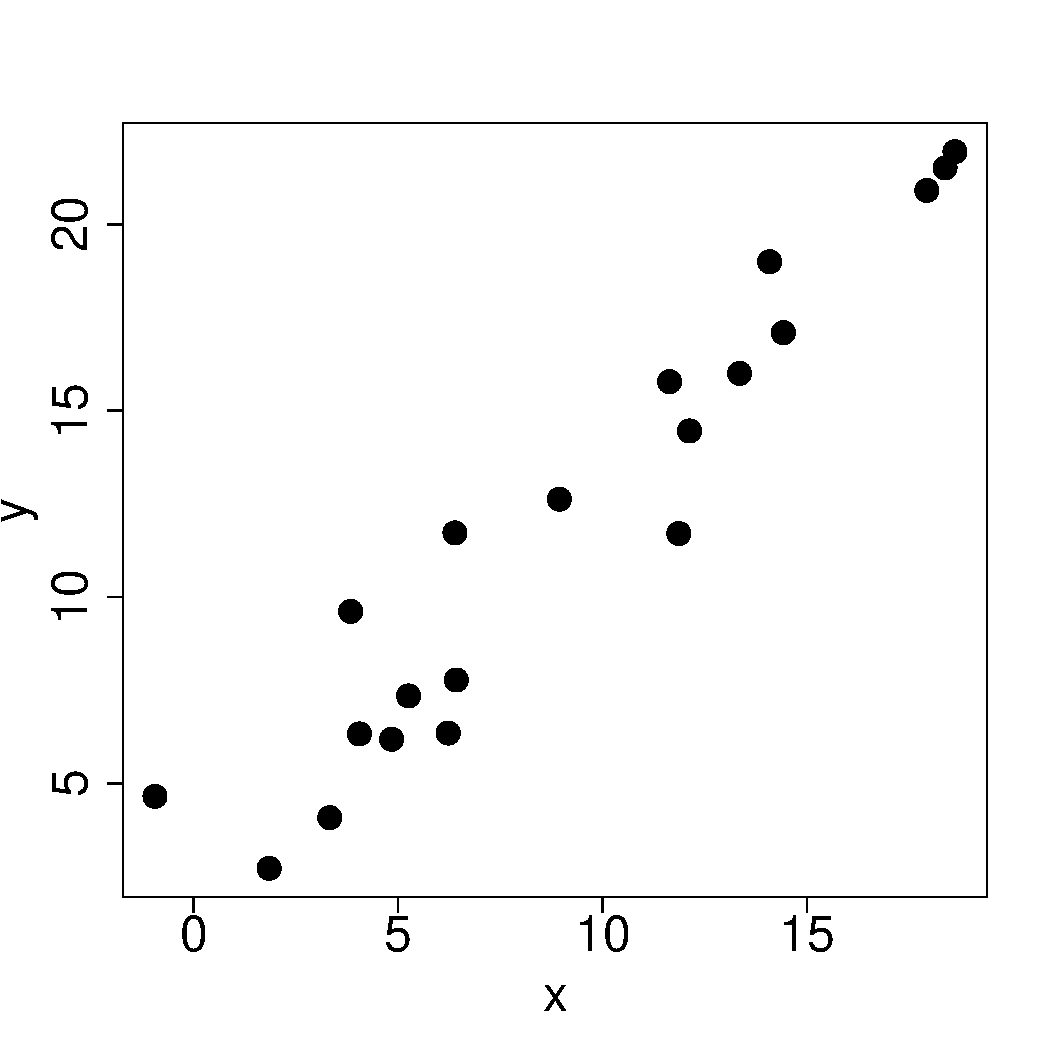
\includegraphics[height=0.7\textheight]{graphics/corrplot}
  \end{center}
\end{frame}


\begin{frame}
  {Kovarianz | Illustration 1}
  Koordinate von $\langle\bar{x},\bar{y}\rangle$ | Mittel der beiden gemessenen Variablen\\
  \begin{center}
    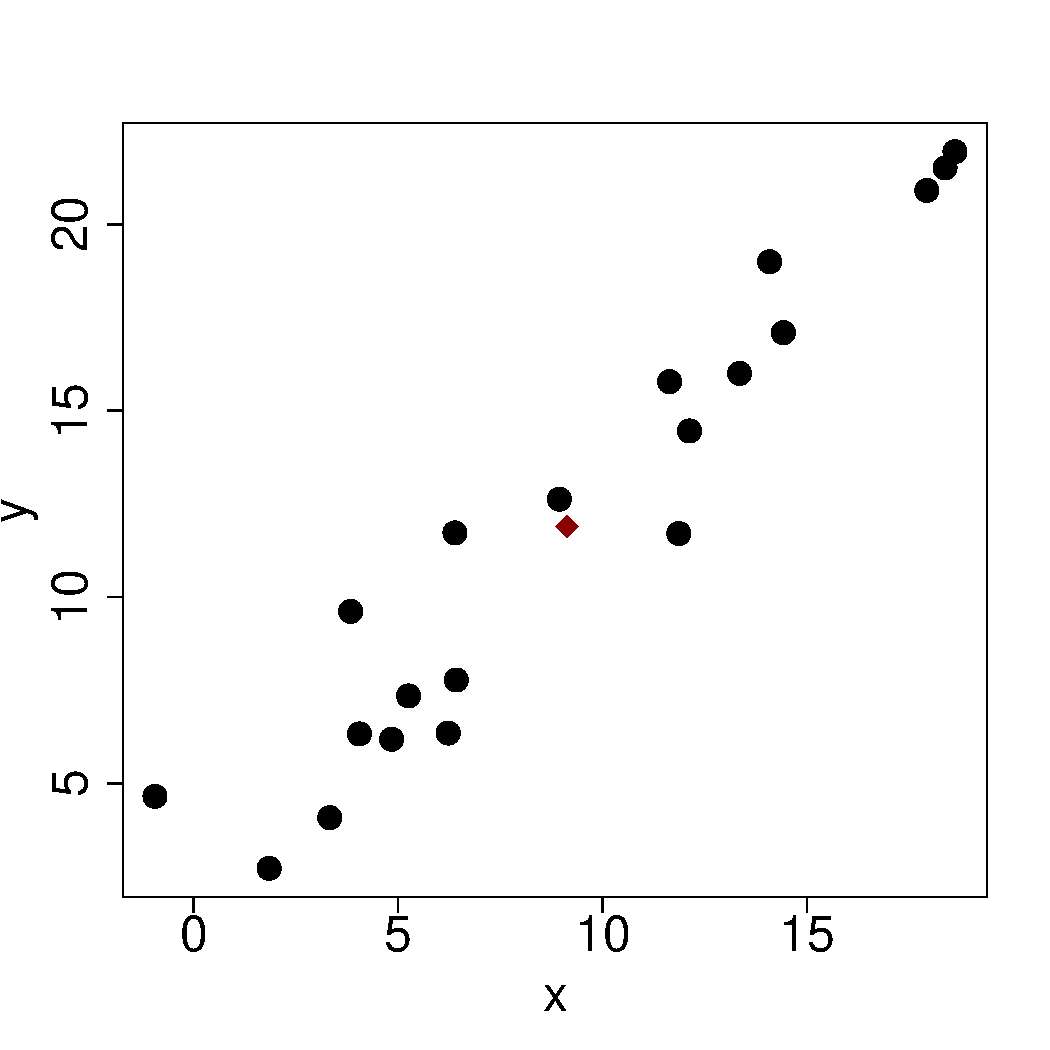
\includegraphics[height=0.7\textheight]{graphics/cov02}
  \end{center}
\end{frame}


\begin{frame}
  {Kovarianz | Illustration 2}
  Punktvarianzen | $x_3-\bar{x}=-7.81$ und $y_3-\bar{y}=-5.80$ | \alert{$-7.81\cdot-5.80=45.30$}\\
  \begin{center}
    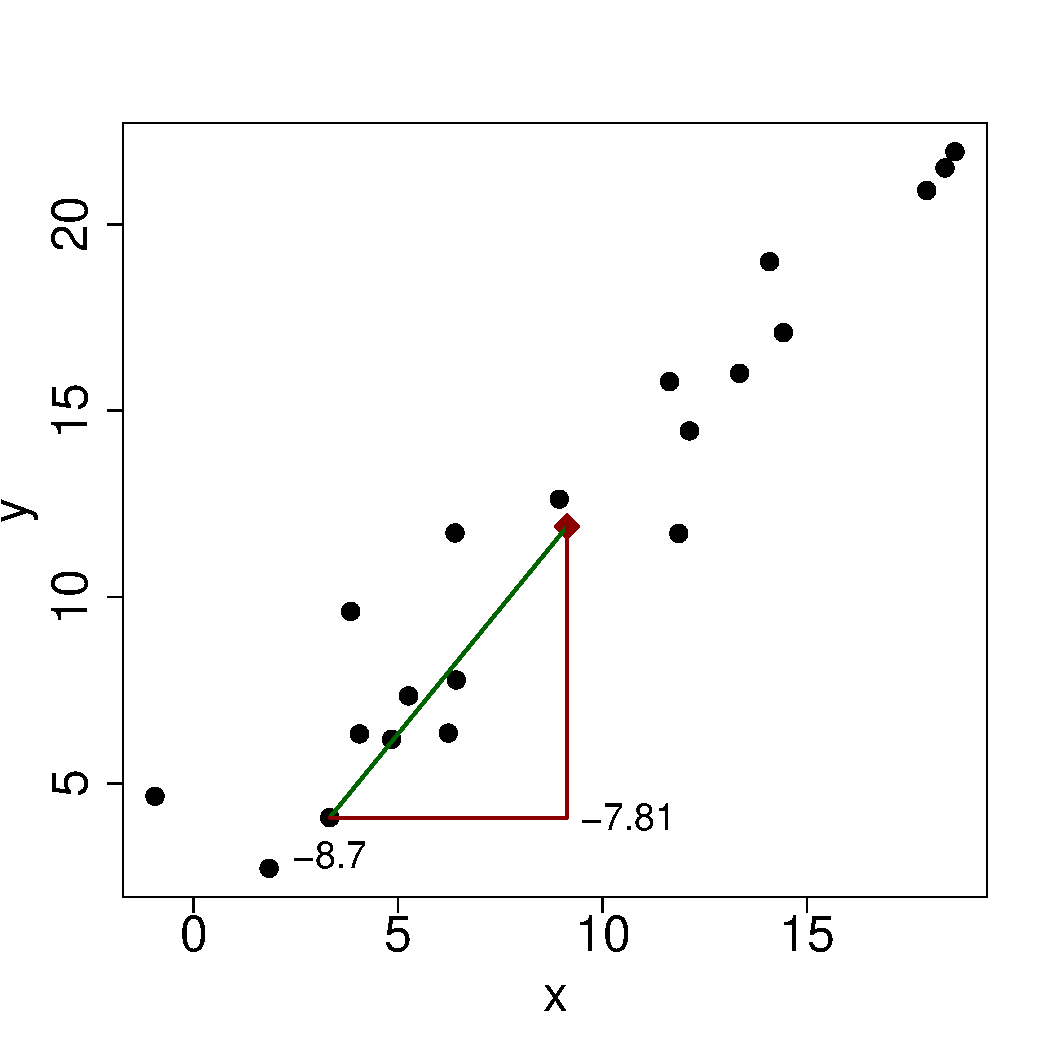
\includegraphics[height=0.7\textheight]{graphics/cov03}
  \end{center}
\end{frame}


\begin{frame}
  {Kovarianz | Illustration 3}
  Punktvarianzen | $x_{17}-\bar{x}=4.95$ und $y_{17}-\bar{y}=7.11$ | \alert{$4.95\cdot7.11=35.19$}\\
  \begin{center}
    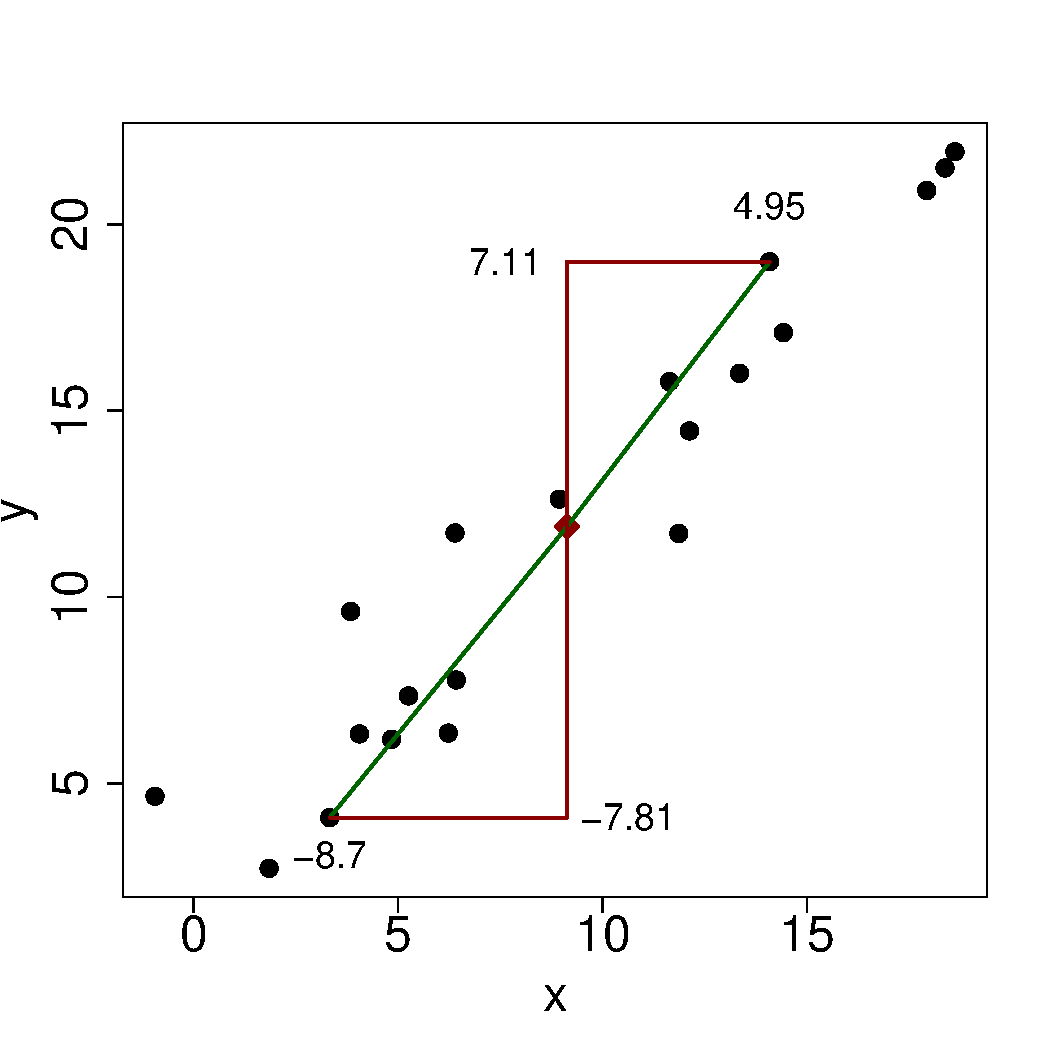
\includegraphics[height=0.7\textheight]{graphics/cov04}
  \end{center}
\end{frame}


\begin{frame}
  {Kovarianz | Illustration 4}
  Puntvarianzen für alle $\langle x_i,y_i\rangle$ \ $cov(x,y)=34.52$\\
  \begin{center}
    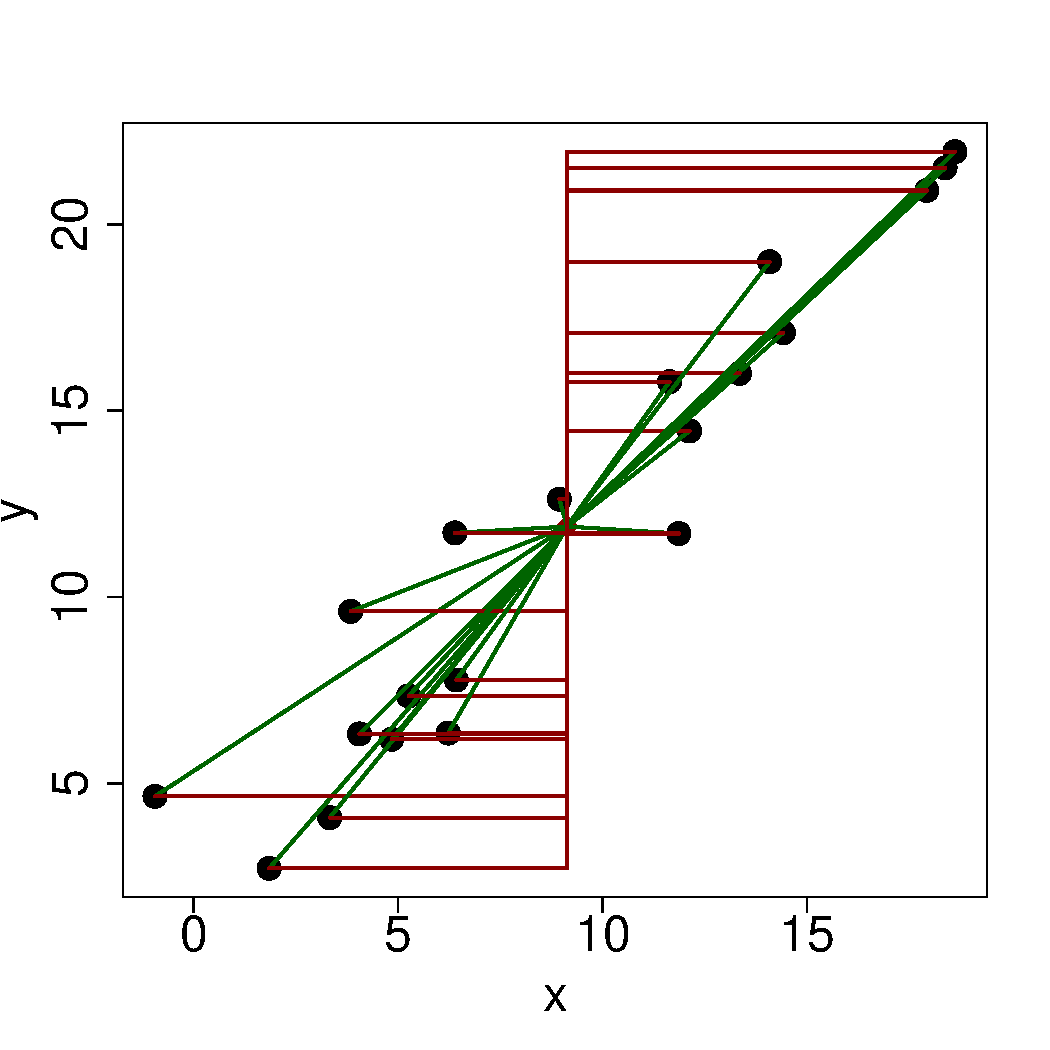
\includegraphics[height=0.7\textheight]{graphics/cov05}
  \end{center}
\end{frame}


\begin{frame}
  {Kovarianz | Illustration 5}
  Ausreißer bei ansonsten positiver Kovarianz | \alert{Negatives Produkt} der Punktvarianzen\\
  \begin{center}
    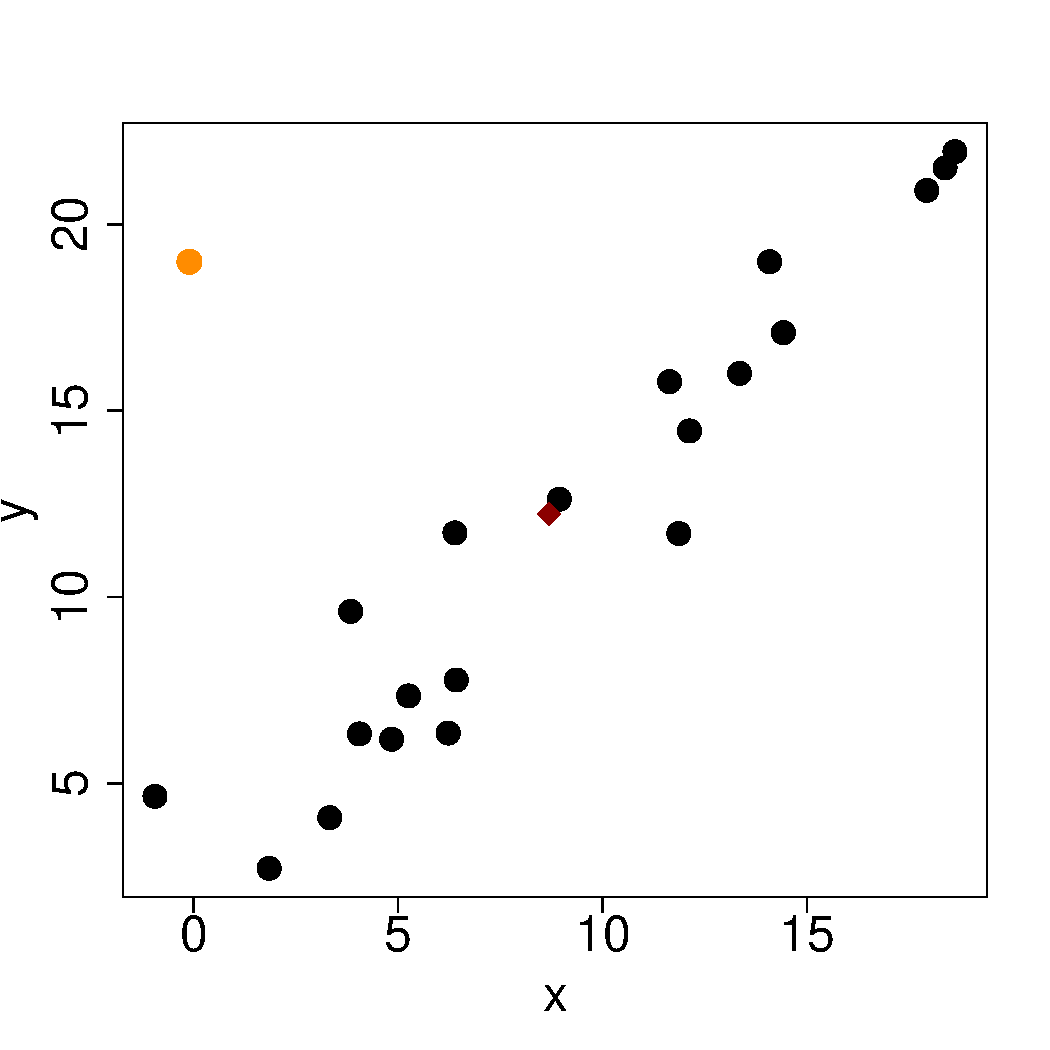
\includegraphics[height=0.7\textheight]{graphics/cov06}
  \end{center}
\end{frame}


\begin{frame}
  {Kovarianz | Illustration 6}
  Punktvarianzen | $x_{21}-\bar{x}=6.77$ und $y_{21}-\bar{y}=-8.79$ | \alert{$6.77\cdot-8.79=-59.51$}\\
  \begin{center}
    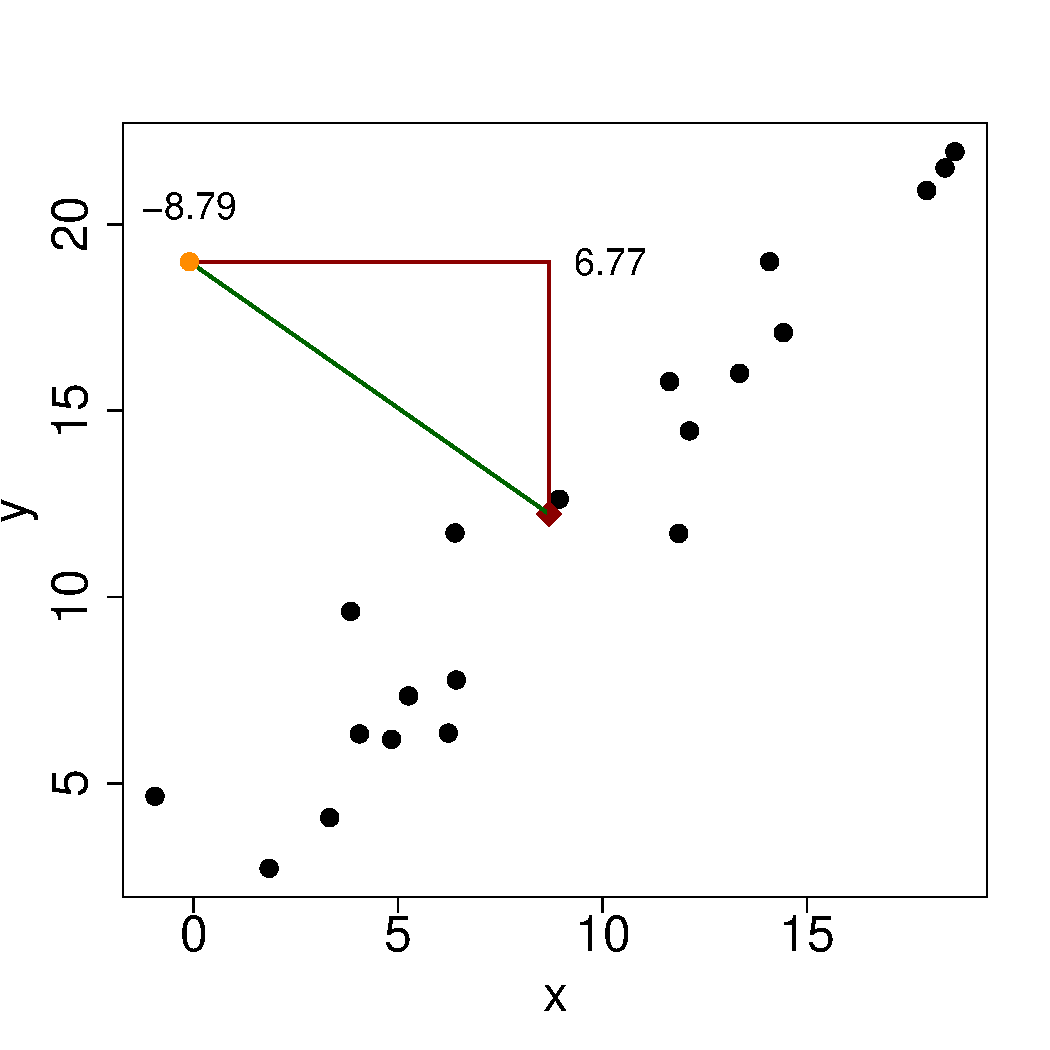
\includegraphics[height=0.7\textheight]{graphics/cov07}
  \end{center}
\end{frame}

\begin{frame}
  {Negative Kovarianz}
  Tendenziell negative Abhängigkeit | Punktvarianzen überwiegend | $cov(x,y)=-33.77$\\
  \begin{center}
    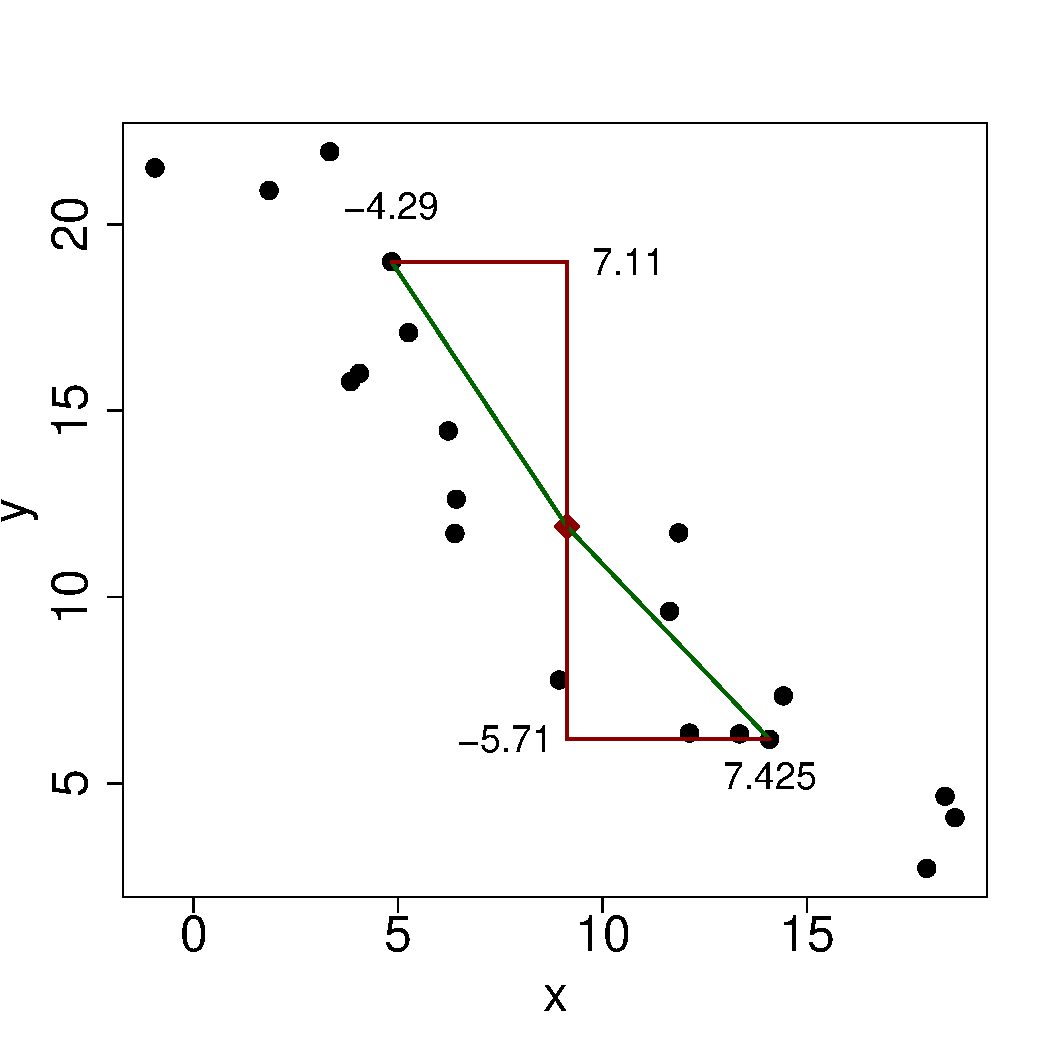
\includegraphics[height=0.7\textheight]{graphics/cov08}
  \end{center}
\end{frame}

\begin{frame}
  {Kovarianz nahe Null}
  Ohne Abhängigkeit | Kovarianz nahe 0 |$cov(x,y)=-1.74$\\
  \begin{center}
    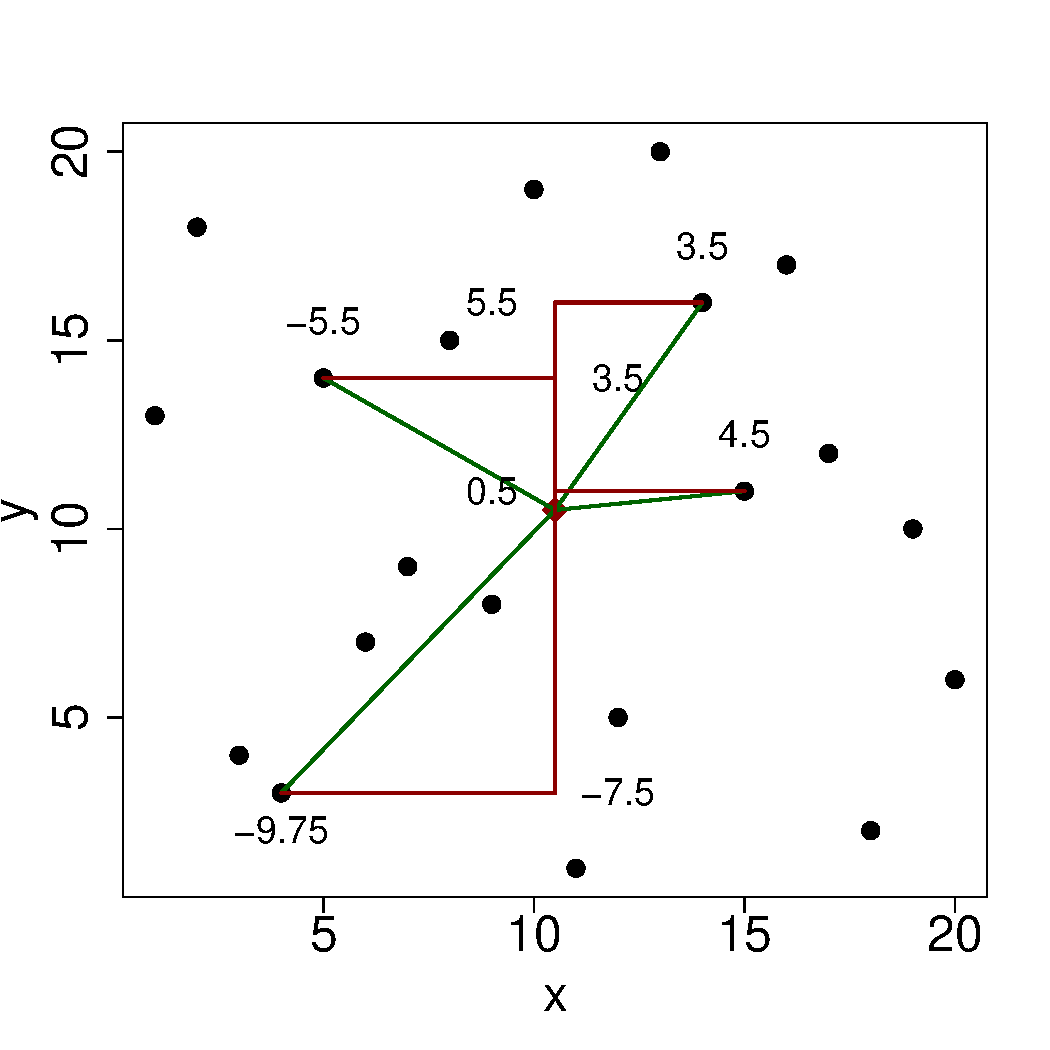
\includegraphics[height=0.7\textheight]{graphics/cov09}
  \end{center}
\end{frame}

\begin{frame}
  {Kovarianz}
  \alert{Kovarianz} | Kombination der Abweichung der Messpunkte vom jeweiligen Mittel\\
  \begin{center}
    \alert{$cov(x,y)=\frac{\sum\limits_{i=1}^{n}(x_i-\bar{x})\cdot(y_i-\bar{y})}{n-1}$}\\
    \Halbzeile
    \alert{Summe der Produkte} | Der Zählerterm | $SP(x,y)=\sum\limits_{i=1}^{n}(x_i-\bar{x})\cdot(y_i-\bar{y})$
  \end{center}
  \Halbzeile
  \begin{itemize}[<+->]
    \item \gruen{$x_i-\bar{x}>0$} und \gruen{$y_i-\bar{y}>0$} | Beitrag zur Kovarianz \gruen{positiv}
    \item \orongsch{$x_i-\bar{x}<0$} und \orongsch{$y_i-\bar{y}<0$} | Beitrag zur Kovarianz \gruen{positiv}
      \Halbzeile
    \item \gruen{$x_i-\bar{x}>0$} und \orongsch{$y_i-\bar{y}<0$} | Beitrag zur Kovarianz \orongsch{negativ}
    \item \orongsch{$x_i-\bar{x}<0$} und \gruen{$y_i-\bar{y}>0$} | Beitrag zur Kovarianz \orongsch{negativ}
  \end{itemize}
\end{frame}



\begin{frame}
  {Korrelationskoeffizient}
  \alert{Korrelationskoeffizient} | Im Gegensatz zur Kovarianz \alert{skalenunabhängig}\\
  \vspace{3\baselineskip}
  \begin{center}
    $r(x,y)=\frac{cov(x,y)}{s(x)\cdot s(y)}$\\
    \Zeile
    \grau{Pearson-Korrelation}
  \end{center}
\end{frame}




% \begin{frame}
%   {Pearson-Korrelation (Wh.)}
%   \begin{center}
%     \alert{$r(x_1,x_2)=\frac{cov(x_1,x_2)}{s(x_1)\cdot s(x_2)}$}
%   \end{center}
%   \pause
%   In Gravetter \& Wallnau, Kap.\ 16 lautet die Formel:
%   \begin{center}
%     \alert{$r=\frac{SP}{\sqrt{SQ_x\cdot SQ_y}}$}
%   \end{center}
%   Die Formeln sind äquivalent, weil (mit $x,y$ statt $x_1,x_2$):
%   \begin{center}
%     $r(x,y)=\frac{cov(x,y)}{s(x)\cdot s(y)}=\onslide<3->{\frac{\frac{\sum(x_i-\bar{x})\cdot(y_i-\bar{x})}{n-1}}{\sqrt{\frac{\sum(x_i-\bar{x})}{n-1}\cdot\frac{\sum(y_i-\bar{y})}{n-1}}}=}\onslide<4->{\frac{\frac{SP(x,y)}{n-1}}{\sqrt{\frac{\sum(x_i-\bar{x})\cdot\sum(y_i-\bar{y})}{n-1}}}=}$\\[3ex]
%     $\onslide<5->{\frac{\frac{SP(x,y)}{n-1}}{\ \ \ \frac{\sqrt{\sum(x_i-\bar{x})\cdot\sum(y_i-\bar{y})}}{n-1}\ \ \ }=}\onslide<6->{\frac{SP(x,y)}{n-1}\cdot\frac{n-1}{\sqrt{SQ(x)\cdot SQ(y)}}=}\onslide<7->{\frac{SP(x,y)}{\sqrt{SQ(x)\cdot SQ(y)}}}$
%   \end{center}
% \end{frame}

\begin{frame}
  {$r^2$ und Siginifikanztests}
  \begin{itemize}[<+->]
    \item Maß der Varianzerklärung durch $r$: \alert{$r^2$} (vgl. t-Test)
    \item \alert{Signifikanztest} möglich: Schluss auf Korrelation in der Grundgesamtheit
    \item $df_r=n-2$
    \item Unter der \Null\ (keine Korrelation) t-verteilt:\\
      \alert{$t=r\sqrt{\frac{n-2}{1-r^2}}$}
    \item \dots oder Tabellen (\zB\ G\&W, B.6)
  \end{itemize}
\end{frame}

\begin{frame}
  {Voraussetzungen}
  \begin{itemize}[<+->]
    \item \alert{Intervallskalierung}
    \item \alert{lineare} Abhängigkeit
    \item bei kleinen $n$: \alert{Normalverteilung} für $x$ und $y$
      \vspace{1cm}
    \item wenn nicht: \alert{Spearmans Rang-Korrelation}
  \end{itemize}
\end{frame}

\begin{frame}
  {Spearmans Rang-Korrelation}
  \begin{itemize}[<+->]
    \item mathematisch \alert{nicht andere als eine Pearson-Korrleation}
    \item vorher: Umrechnung der rohen x,y-Werte in \alert{Ränge}
    \item bei gleichen Werten: \alert{alle gleichen Werte bekommen Rang-Mittel}
  \end{itemize}
\end{frame}

\begin{frame}
  {Werte in Ränge umrechnen}
  Ein Beispiel zur Umwandlung in Ränge:
  \begin{center}
    \begin{tabular}[h!]{|c||c|c|c|c|c|}
      \hline
      Index: & 1 & 2 & 3 & 4 & 5 \\
      \hline
      \hline
      Messwerte x:& 4 & 7 & 3 & 1 & 3 \\
      \hline
      Messwerte y: & 9 & 12 & 11 & 2 & 8 \\
      \hline
    \end{tabular}
  \end{center}
  Statt der Messwerte arbeitet man mit den Rängen der Messwerte an den jeweiligen Indexen.
  \begin{center}
    \begin{tabular}[h!]{|c||c|c|c|c|c|}
      \hline
      Index: & 1 & 2 & 3 & 4 & 5 \\
      \hline
      \hline
      Ränge der Messwerte x:& 4 & 5 & 2.5 & 1 & 2.5 \\
      \hline
      Ränge der Messwerte y: & 3 & 5 & 4 & 1 & 2 \\
      \hline
    \end{tabular}
  \end{center}
\end{frame}

\begin{frame}
  {Abkürzung der Berechnung}
  Wenn $Rang(x_i)$ der Rang für $x_i$ in $x$ ist:\\
  \vspace{0.5cm}
  \begin{center}
    Spearmans Rang-Korrelation:\\[2ex]
    \alert{$r_{S}=1-\frac{6\sum\limits_{i=1}^n(Rang(x_i)-Rang(y_i))^2}{n(n^2-1)}$}
  \end{center}
\end{frame}

\subsection{Lineare Regression}

\begin{frame}
  {Unterschiede zwischen Korrelation und Regression}
  \begin{itemize}[<+->]
    \item Korrelation: Stärke des Zusammenhangs
    \item \alert{Regression: genaue Funktion zur Modellierung des Zusammenhangs}
      \vspace{0.5cm}
    \item Korrelation: Diagnostik\slash Test
    \item \alert{Regression: Vorhersage} (und Test)
  \end{itemize}
\end{frame}

\begin{frame}
  {Spezifikation der Funktion für die Regressionsgerade}
  \vspace{-0.5cm}
  \begin{center}
    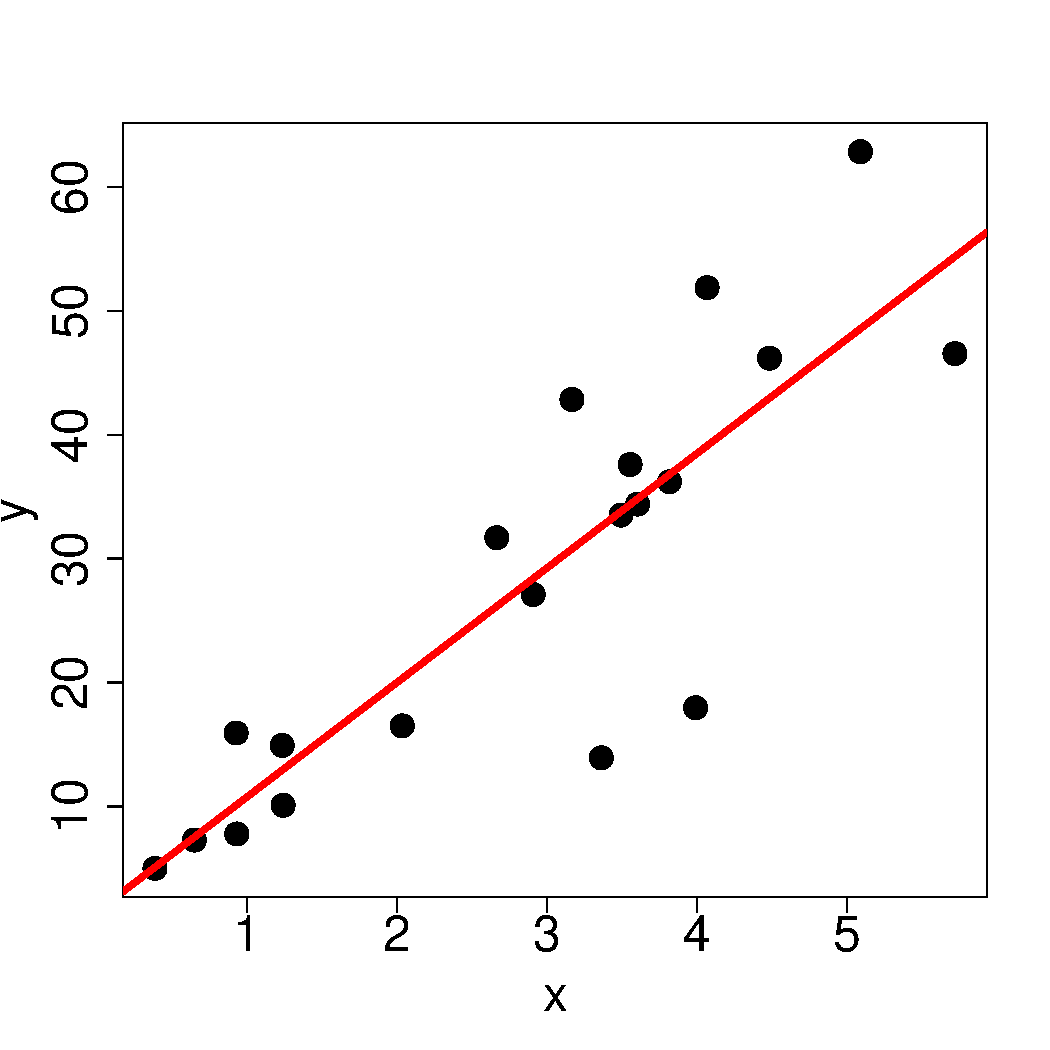
\includegraphics[width=0.3\textwidth]{graphics/regline}
  \end{center}
  \vspace{-0.5cm}
  \pause
  \begin{itemize}[<+->]
    \item Schnittpunkt mit der y-Achse (\alert{Intercept}): \alert{$a$}
    \item Steigung (\alert{Slope}): \alert{$b$} ($b$ heißt auch \alert{Koeffizient}) 
    \item \alert{Regressiongleichung (=Modell): $\hat{y}=b\cdot x+a$}
    \item Für jeden beobachteten Wert: \alert{$y_i=b\cdot x_i+a+e_i$} ($e_i$ als Fehlerterm)
  \end{itemize}
\end{frame}

\begin{frame}
  {Idee der kleinsten Quadrate}
  Die vom Modell vorhergesagten Werte (rot, auf der Regressionsgerade)\\
  sollen insgesamt einen so geringen Abstand wie möglich\\
  zu den Beobachtungen (blau) haben.
  \vspace{-0.5cm}
  \begin{center}
    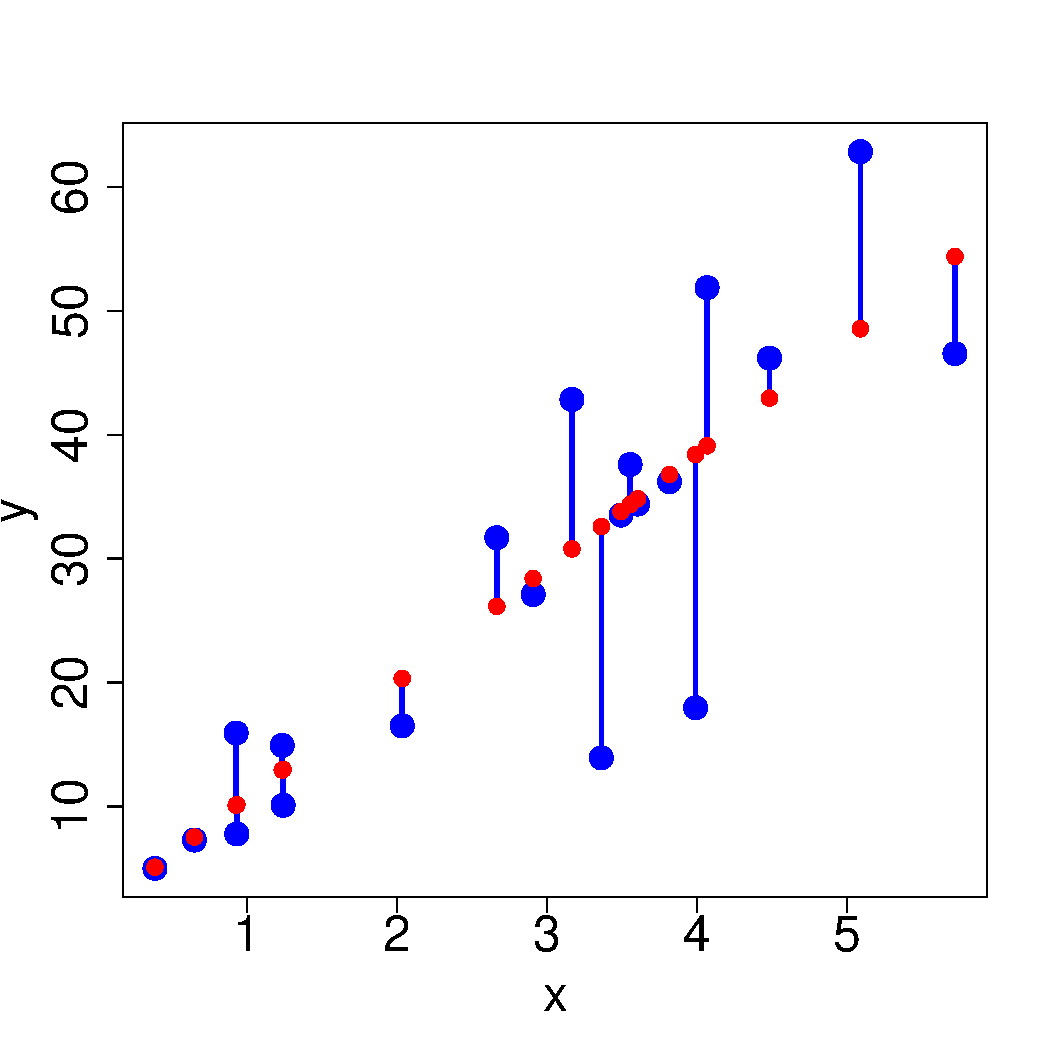
\includegraphics[width=0.3\textwidth]{graphics/lmerrors}
  \end{center}
  \pause
  Die Summe der \alert{quadrierten} negativen und positiven Differenzen (blau)\\
  soll \alert{minimiert} werden (=kleinste Quadrate): Minimierung von \alert{$E=\sum e^2$}
\end{frame}

\begin{frame}
  {Berechnung der Regressionsgleichung}
  \begin{itemize}[<+->]
    \item Slope\slash Steigung: $\alert{b=\frac{\sum(x_i-\bar{x})\cdot(y_i-\bar{y})}{\sum(x_i-\bar{x})^2}}=\frac{SP(x,y)}{SQ(x)}$
      \vspace{0.5cm}
    \item Intercept: $\alert{a=\bar{y}-b\cdot\bar{x}}$
      \vspace{0.5cm}
    \item Der Beweis, dass dies die Gerade mit den kleinsten Quadraten schätzt,
      erfordert bereits erheblichen mathematischen Aufwand, den wir uns sparen.
      \vspace{0.5cm}
    \item Determinationskoeffizient: \alert{$r^2=\frac{\sum(\hat{y}_i-\bar{y})^2}{\sum(y_i-\bar{y})^2}$}
    \end{itemize}
\end{frame}

\begin{frame}
  {Standardfehler für die Gleichung}
  \begin{itemize}[<+->]
    \item Wie stark variiert der Fehler für Stichproben einer Größe?
      \vspace{0.5cm}
    \item \alert{$SF_{residual}=\sqrt{\frac{\sum e^2}{n-2}}$}
      \vspace{0.5cm}
    \item Je kleiner $SF_{residual}$, desto besser das Modell.
    \item Beachte: $n$ wird größer (größere Stichprobe): $SF_{residual}$ wird kleiner.
    \item Und: Fehler $e$ werden kleiner: $SF_{residual}$ wird kleiner.
  \end{itemize}
\end{frame}

\begin{frame}
  {F-Test für Model}
  \begin{itemize}[<+->]
    \item Wie bei ANOVA: \alert{$F=\frac{erklaerte\ Varianz}{zufaellige\ Varianz}=\frac{s^2_{regression}}{s^2_{residual}}$}
      \vspace{0.5cm}
    \item zufällige Varianz: \alert{$s^2_{residual}=\frac{(1-r^2)\cdot SQ(y)}{1}$}
    \item erklärte Varianz: \alert{$s^2_{regression}=\frac{r^2\cdot SQ(y)}{n-2}$}
      \vspace{0.5cm}
    \item Freiheitsgrade sind immer $df_1=1$ und $df_2=n-1$.
    \item Beachte: $r^2$ ist in $[0..1]$ und teilt die Varianz von $y$ auf.
  \end{itemize}
\end{frame}

\begin{frame}
  {Standardfehler und t-Test für Koeffizienten}
  \begin{itemize}[<+->]
    \item Für $b$ und $a$ kann je ein Standardfehler angegeben werden. 
      \vspace{0.5cm}
    \item \alert{$SF(b)=\frac{\sqrt{\frac{\sum e^2}{n-1}}}{\sqrt{SQ(x)}}$}
      \vspace{0.5cm}
    \item Unter der \Null: $b=0$ ist dann t-verteilt:\\
      \alert{$t=\frac{b}{SF(b)}$}
  \end{itemize}
\end{frame}

\subsection{Multiple Regression}

\begin{frame}
  {Mehrere unabhängige}
  \begin{itemize}[<+->]
    \item Design bei einfachem LM:
      \begin{itemize}[<+->]
	\item \alert{eine intervallskalierte Abhängige}
	\item \alert{eine Unabhängige}
      \end{itemize}
      \vspace{0.5cm}
    \item wie bei mehrfaktorieller ANOVA:
      \begin{itemize}[<+->]
	\item oft interessiert \alert{mehrfaktorielle Abhängigkeit}
      \end{itemize}
  \end{itemize}
\end{frame}

\begin{frame}
  {Multivariate Modellgleichung}
  Mehrere Koeffizienten im \alert{allgemeinen linearen Modell}:\\
  \pause
  \vspace{0.5cm}
  \begin{center}
    \alert{$\hat{y}=b_1\cdot x_1+b_2\cdot x_2\dots b_n\cdot x_n+a$}
  \end{center}
  \vspace{0.5cm}
  \pause
  Konzeptuell bleibt die Berechnung aller Werte und Tests gleich,\\
  die Mathematik wird ungleich komplizierter.\\
  \vspace{0.5cm}
  \pause
  Man schreibt \alert{$R^2$} statt $r^2$.
\end{frame}

\begin{frame}
  {Normalitätsannahme}
  \begin{center}
    \alert{Die Residuen $E$ müssen normalverteilt sein.}\\
    (als Diagnostik für: \alert{Die Messwerte müssen normalverteilt sein.})
  \end{center}
  \begin{itemize}[<+->]
    \item Missverständnis: Test aller Residuen auf Normalität
    \item denn: \alert{Für jedes $x_i$ müssen die $e$ normalverteilt sein.}
    \item erfordert mehrere Messungen pro $x_i$ oder Intervallbildung 
    \item größere Stichproben, kleinere Probleme
    \item visuelle Diagnose: Q-Q-Plots (hier nicht behandelt)
  \end{itemize}
\end{frame}

\begin{frame}
  {Unabhängigkeit}
  \begin{center}
    \alert{Jedes $y_i$ darf nur von $x_i$ abhängen,\\
        niemals zusätzlich von $x_j$ mit $i\neq j$.}
  \end{center}
  \begin{itemize}[<+->]
    \item mathematisch: nicht-lineare Abhängigkeit
    \item konzeptuell: Zeitserien
    \item konzeptuell: Sequenzen in Texten
    \item Lösung: andere Modellspezifikation
  \end{itemize}
\end{frame}

\begin{frame}
  {Homoskedastizität}
  \begin{center}
    \alert{Die Residuen müssen homoskedastisch verteilt sein.}
  \end{center}
  \begin{itemize}[<+->]
    \item Bedeutung: Die Varianz der $e$ muss über alle $x$ homogen sein.
    \item vgl.\ die Forderung der "`Varianzhomogenität"' bei t-Test und ANOVA
  \end{itemize}
\end{frame}

\begin{frame}
  {Darstellung heteroskedastischer Residuen}
  Hier wird die Varianz der Residuen mit steigendem x immer größer.\\
  Ein lineares Modell versagt hier wegen verletzter Verteilungsannahmen.
  \begin{center}
    \includegraphics[width=0.4\textwidth]{graphics/hetresid}
  \end{center}
\end{frame}

\begin{frame}
  {Lösung von LM-Krisen}
  \begin{itemize}[<+->]
    \item mehr Daten ziehen, Daten transformieren
      \vspace{0.5cm}
    \item \alert{generalisierte lineare Modelle (GLM)}\\
      legen andere Verteilungsannahmen zugrunde
      \vspace{0.5cm}
    \item (generalisiert) additive Modelle (GAM)\\
      schätzen Smoothingfunktionen für Koeffizienten
  \end{itemize}
\end{frame}

\subsection{ANOVA und LMs}

\begin{frame}
  {ANOVA als Modell mit kategorialen Regressoren}
  $n$ Gruppen der ANOVA können als $n$ dichotome Variablen dargestellt werden:\\
  \vspace{0.5cm}
  \begin{center}
    \begin{tabular}[h!]{|c|c|c|c|c|}
      \cline{3-5}
      \multicolumn{2}{c|}{} & \multicolumn{3}{c|}{\textbf{ANOVA-Gruppen}} \\
      \cline{3-5}
      \multicolumn{2}{c|}{} & $A_1$ & $A_2$ & $A_3$ \\
      \hline
      \multirow{3}{*}{\begin{sideways}\textbf{Regressor}\end{sideways}} & \rule{0em}{2em} $x_1=$ & $\mathbf{1}$ & $0$ & $0$ \\
      \cline{2-5}
      & \rule{0em}{2em} $x_2=$ & $0$ & $\mathbf{1}$ & $0$ \\
      \cline{2-5}
      & \rule{0em}{2em} $x_3=$ & $0$ & $0$ & $\mathbf{1}$ \\
      \hline
    \end{tabular}
  \end{center}
\end{frame}

\begin{frame}
  {Lineares Modell mit solchen "`Dummy-Variablen"'}
  Normale Modellspezifikation:

  \begin{center}
    $\hat{y}=b_1x_1 + b_2x_2 + \cdots + b_nx_n + a$
  \end{center}
  \vspace{0.5cm}
  \pause
  \begin{center}
    Da jeweils nur eins der $x_i=1$ und alle anderen immer $0$ werden,\\
    wird einfach der Wert des entsprechenden $\beta_i$ (plus $a$) vorhergesagt.
  \end{center}
\end{frame}

%\begin{frame}
%  {Kleinste Quadrate bei Gruppen-Design}
%  Die kleinsten Quadrate erhält man in einem Design mit nominalen Abhängigen,\\
%  wenn man jeweils das Gruppen-Mittel vorhersagt.\\[03ex]
%  Wir setzen diese als Koeffizienten ein und setzen zunächst $a=0$.
%  \vspace{0.5cm}
%  \pause
%  \begin{center}
%    $\hat{y}=\bar{y_1}x_1 + \bar{y_2}x_2 + \cdots + \bar{y_n}x_n$
%  \end{center}
%  \vspace{0.5cm}
%  \pause
%  Zusätzlich kann man als Intercept das Gesamtmittel $\bar{Y}$ einsetzen\\
%  und die Koeffizienten als Abweichung vom Gesamtmittel definieren.
%  \begin{center}
%    $\hat{y}=(\bar{y_1}-\bar{Y})x_1 + (\bar{y_2}-\bar{Y})x_2 + \cdots + (\bar{y_n}-\bar{Y})x_n + \bar{Y}$
%  \end{center}
%\end{frame}
%
%\begin{frame}
%  {Beispiel}
%  Wenn $x_2=1$ (und folglich $x_1=0$ und $x_3=0$):
%  \begin{center}
%    \begin{equation}
%      \begin{split}
%	\hat{y} & = (\bar{y_1}-\bar{Y})0 + (\bar{y_2}-\bar{Y})1 + \cdots + (\bar{y_n}-\bar{Y})0 + \bar{Y}\\
%	 &= 0 + (\bar{y_2}-\bar{Y}) + \cdots + 0 + \bar{Y} \\
%	 &= \bar{y_2} - \bar{Y} + \bar{Y} \\
%	 &= \bar{y_2}
%      \end{split}
%    \end{equation}
%  \end{center}
%  \pause
%  Als Vorhersagewert kommt also einfach das $y$-Mittel der Gruppe\\
%  zum eingegebenen $x$ heraus.
%\end{frame}
%
%\begin{frame}
%  {F-Signifikanztest mit Modell-Residuen}
%  Für ein voll spezifiziertes Modell
%  \begin{center}
%    $\hat{y_f}=(\bar{y_1}-\bar{Y})x_1 + (\bar{y_2}-\bar{Y})x_2 + \cdots + (\bar{y_n}-\bar{Y})x_n + \bar{Y}$
%  \end{center}
%  \pause
%  und ein reduziertes Modell (ohne Informationen über Gruppen-Mittel)
%  \begin{center}
%    $\hat{y_r}=\bar{Y}$
%  \end{center}
%  \pause
%  können nun die Summen der Residuen verglichen werden:
%  \begin{center}
%    \alert{$F=\frac{\ \ \frac{E_r-E_f}{df_r-df_f}\ \ }{\frac{E_f}{df_f}}=\frac{\text{erklärte Varianz}}{\text{zufällige Varianz}}$}\\
%    $E_f$ = Residuen des vollen Modells, $E_r$ = Residuen des reduzierten Modells
%  \end{center}
%\end{frame}

\subsection{In \texttt{R}}

\begin{frame}
  {Spearmans Rang-Korrleation in \texttt{R}}
  Die Funktion \texttt{cor()} hat ein Argument \texttt{method},\\
  das als \texttt{"{}spearman"} angegeben werden kann.\\
  \begin{center}
    \texttt{> cor(x, y, method = "{}spearman")}
  \end{center}
\end{frame}

\begin{frame}
  {Lineare Modelle in \texttt{R}}
  \begin{itemize}[<+->]
    \item Modellformeln: \alert{\texttt{y\textasciitilde}x}\\
      "`y abhängig von x"'
    \item Mehrere Unabhängige: \alert{\texttt{y\textasciitilde x1+x2}}
    \item Mehrere Unabhängige mit \alert{Interaktion}: \alert{\texttt{y\textasciitilde x1*x2}}
    \item Mehrere Unabhängige \alert{nur Interaktion}: \alert{\texttt{y\textasciitilde x1:x2}}
      \vspace{0.5cm}
    \item Lineares Modell schätzen und speichern:\\
      \alert{\texttt{> m <- lm(y\textasciitilde x)}}
    \item Ausgabe Evaluation:\\
      \alert{\texttt{> summary(m)}}
  \end{itemize}
\end{frame}

\begin{frame}
  {Ausgabe LM}
  Interpretieren Sie diese Ausgabe anhand der Folien:\\
  \begin{center}
    \scalebox{0.7}{
    \begin{boxedminipage}{1.2\textwidth}
      \ttfamily
Call:\\
lm(formula = y \~{ } x)\\

Residuals:\\
\ \ \ \ \ Min\ \ \ \ \ \ \ 1Q\ \ \ Median\ \ \ \ \ \ \ 3Q\ \ \ \ \ \ Max\ \\
-20.4298\ \ -2.4920\ \ -0.2625\ \ \ 3.8038\ \ 14.2922\ \\

Coefficients:\\
\ \ \ \ \ \ \ \ \ \ \ \ Estimate\ Std.\ Error\ t\ value\ Pr(>|t|)\ \ \ \ \\
(Intercept)\ \ \ \ 1.513\ \ \ \ \ \ 4.321\ \ \ 0.350\ \ \ \ \ 0.73\ \ \ \ \\
x\ \ \ \ \ \ \ \ \ \ \ \ \ \ 9.242\ \ \ \ \ \ 1.333\ \ \ 6.933\ 1.77e-06\ ***\\
---\\
Signif.\ codes:\ \ 0\ ‘***’\ 0.001\ ‘**’\ 0.01\ ‘*’\ 0.05\ ‘.’\ 0.1\ ‘\ ’\ 1\\

Residual\ standard\ error:\ 9.008\ on\ 18\ degrees\ of\ freedom\\
Multiple\ R-squared:\ \ 0.7275,	Adjusted\ R-squared:\ \ 0.7124\ \\
F-statistic:\ 48.06\ on\ 1\ and\ 18\ DF,\ \ p-value:\ 1.768e-06\ \\
    \end{boxedminipage}}
  \end{center}
\end{frame}

%\begin{frame}
%  {ANOVA in \texttt{R}}
%  Beispiel: zweifaktoriella ANOVA mit Faktor A und B und Interaktion.
%  \begin{itemize}[<+->]
%    \item Modell spezifizieren:\\
%      \alert{\texttt{> m <- lm(x\textasciitilde A*B)}}
%    \item ANOVA rechnen\slash speichern:\\
%      \alert{\texttt{> a <- aov(m)}}
%    \item Ausgabe:\\
%      \alert{\texttt{> summary(a)}}
%  \end{itemize}
%\end{frame}
%
%\begin{frame}
%  {Ausgabe ANOVA}
%  \begin{center}
%    \scalebox{0.7}{
%    \begin{boxedminipage}{1.2\textwidth}
%      \ttfamily
%\ \ \ \ \ \ \ \ \ \ \ \ \ Df\ Sum\ Sq\ Mean\ Sq\ F\ value\ \ \ Pr(>F)\ \ \ \\ \
%A\ \ \ \ \ \ \ \ \ \ \ \ 1\ \ \ 0.38\ \ \ \ 0.38\ \ \ 0.094\ 0.762577\ \ \ \ \\
%B\ \ \ \ \ \ \ \ \ \ \ \ 2\ \ \ 6.25\ \ \ \ 3.12\ \ \ 0.784\ 0.471570\ \ \ \ \\
%A:B\ \ \ \ \ \ \ \ \ \ 2\ 105.25\ \ \ 52.62\ \ 13.202\ 0.000296\ ***\ \\
%Residuals\ \ \ 18\ \ 71.75\ \ \ \ 3.99\ \ \ \ \ \ \ \ \ \ \ \ \ \ \ \ \ \ \ \ \ \\
%---\\
%Signif.\ codes:\ \ 0\ ‘***’\ 0.001\ ‘**’\ 0.01\ ‘*’\ 0.05\ ‘.’\ 0.1\ ‘\ ’\ 1\\
%    \end{boxedminipage}}
%  \end{center}
%  Hinweis: Mit \texttt{"{}Mean Sq"} ist $s^2$ gemeint.
%\end{frame}


\section{Lineare Modelle und ANOVA}


\begin{frame}
  {Äquivalenz von ANOVA und LM}
  Binäre Kodierung der Gruppenzugehörigkeit\\
  Hier: drei Gruppen von einem Faktor (einfaktorielle ANOVA mit drei Gruppen)\\

 \begin{center}
   \begin{tabular}[h!]{|c|c|c|c|c|}
     \cline{3-5}
     \multicolumn{2}{c|}{} & \multicolumn{3}{c|}{\textbf{ANOVA-Gruppen}} \\
     \cline{3-5}
     \multicolumn{2}{c|}{} & $A_1$ & $A_2$ & $A_3$ \\
     \hline
     \multirow{3}{*}{\begin{sideways}\textbf{Regressor}\end{sideways}} & \rule{0pt}{18pt} $x_1=$ & $\mathbf{1}$ & $0$ & $0$ \\
     \cline{2-5}
     & \rule{0pt}{18pt} $x_2=$ & $0$ & $\mathbf{1}$ & $0$ \\
     \cline{2-5}
     & \rule{0pt}{18pt} $x_3=$ & $0$ & $0$ & $\mathbf{1}$ \\
     \hline
   \end{tabular}
  \Zeile
   \begin{equation}
    \hat{y}=b_1x_1 + b_2x_2 + \cdots + b_nx_n + a
  \end{equation}
 \end{center}
\end{frame}


\begin{frame}
  {Volles Modell, Kleinste Quadrate}
  Kleinste Quadrate | für jeden Koeffizienten $b_i$ jeweils Mittelwert der Gruppe $i$ ($\bar{y_i}$)\\
  Außerdem erstmal $a=0$ | dann:\\
  \Halbzeile 
  \begin{equation}
    \hat{y}=\bar{y_1}x_1 + \bar{y_2}x_2 + \cdots + \bar{y_n}x_n
  \end{equation}

  \Zeile
  Allgemeines Mittel als Intercept | $a=\bar{Y}$\\
  Koeffizienten = Abweichung Gruppenmittel vom Gesamtmittel\\
  \Halbzeile  
  \begin{equation}
    \hat{y}=(\bar{y_1}-\bar{Y})x_1 + (\bar{y_2}-\bar{Y})x_2 + \cdots + (\bar{y_n}-\bar{Y})x_n + \mathbf{\bar{Y}}
  \end{equation}
\end{frame}


\begin{frame}
  {Beispiel für einen Datenpunkt aus Gruppe 2}
  Entsprechend in ANOVA $A_2$ | Unabhängige im LM: $x_1=0$, $x_2=1$ und $x_3=0$\\
  Schätzung für den $y$-Wert:\\
  \Halbzeile  
  \begin{equation}
    \begin{split}
      \hat{y} & = (\bar{y_1}-\bar{Y})0 + \mathbf{(\bar{y_2}-\bar{Y})1} + \cdots + (\bar{y_n}-\bar{Y})0 + \mathbf{\bar{Y}}\\
       &= 0 + (\bar{y_2}-\bar{Y}) + \cdots + 0 + \bar{Y} \\
       &= \bar{y_2} - \bar{Y} + \bar{Y} \\
       &= \bar{y_2}
    \end{split}
  \end{equation}
  
  \Zeile
  Jeder $\hat{y}$-Wert | Mittel der beobachteten $y$-Werte der Gruppe, zu der er gehört\\
  \grau{\footnotesize Das ergibt für ausschließlich nominale Unabhängige in der Tat den Schätzer mit den kleinsten Quadraten (s.\ Maxwell \& Delaney, Kap.\ 3).}
\end{frame}

\begin{frame}
  {Test über Modell}
  Kernfrag | \alert{Bringen Abweichungen der Gruppenmittel eine Verbesserung der Vorhersage\\
  gegenüber dem Gesamt-Mittel?}\\
  \Halbzeile
  Methode | Vergleich der \alert{Residuen $E_f$ für volles Modell} (mit Gruppenmitteln)\\
  vs.\ \alert{Residuen $E_r$ für reduziertes Modell} (ohne Gruppenmittel)\\

  \Zeile
  Gleichung~\ref{eq:fullmod} für volles und Gleichung~\ref{eq:redmod} für reduziertes Modell\\
  
  \begin{equation}
      \mathbf{\hat{y_f}}=(\bar{y_1}-\bar{Y})x_1 + (\bar{y_2}-\bar{Y})x_2 + \cdots + (\bar{y_n}-\bar{Y})x_n + \bar{Y}
      \label{eq:fullmod}
  \end{equation}
  
  \begin{equation}
    \mathbf{\hat{y_r}}=\bar{Y}
      \label{eq:redmod}
  \end{equation}
  
\end{frame}

\begin{frame}
  {Vergleich von Varianzen = ANOVA | F-Verteilung}
  \begin{equation}
    F=\frac{\ \ \frac{E_r-E_f}{df_r-df_f}\ \ }{\frac{E_f}{df_f}}=\frac{\text{erklärte Varianz}}{\text{zufällige\ Varianz}}
  \end{equation}

  \Zeile
  \begin{enumerate}
    \item Residuen = Maß für die Varianz
    \item Residuen des vollen Modells = Maß für die Varianz,\\
      die trotz der Erklärungskraft des vollen Modells bleibt (= unerklärte Varianz)
    \item Residuen des reduzierten Modells = Maß für die Gesamtvarianz\\
      (Abweichungen vom Gesamt-Mittel)
    \item Zähler | trotz der Erklärung verbleibende Varianz $-$ vollen Varianz\\
      abgezogen (=  erklärte Varianz)
    \item Quotient insgesamt | Zählervarianz in Bezug zur Gesamtvarianz\\
      (klassischer F-Quotient, s.\ ANOVA)
  \end{enumerate}
\end{frame}

% Dieser Vergleich erfolgt über den folgenden F-Quotienten, mit dem konzeptuell und mathematisch die Konvergenz zur klassischen ANOVA hergestellt wird:
% 
% 
% Alternativ kann man eins der Gruppenmittel zum Referenzmittel (= Intercept) machen.
% Dann evaluiert man die anderen relativ zu diesem.
% Konzeptuell ist das dasselbe.
% 
% In \texttt{R} kann man eine ANOVA folgendermaßen Rechnen und damit eine klassische ANOVA-Ausgabe produzieren (mit \texttt{Mean Sq} meint \texttt{R} einfach die Varianz $s^2$):
% 
% \begin{center}
%   \textbf{\texttt{summary(aov(lm(y\textasciitilde A)))}}
% \end{center}
% 
% \texttt{y} ist dabei ein Vektor, der die beobachteten Werte enthält, und \texttt{A} ein Faktor, der passend dazu die Faktor-Ausprägungen entsprechend der Gruppen paart.
% Als Mini-Beispiel:
% 
% \begin{center}
%   \begin{tabular}[h!]{|c|c|c|}
%     \cline{1-1}\cline{3-3}
%     \textbf{\texttt{y}} && \textbf{\texttt{A}} \\
%     \cline{1-1}\cline{3-3}
%     \multicolumn{1}{c}{} & \multicolumn{1}{c}{} & \multicolumn{1}{c}{}\\
%     \cline{1-1}\cline{3-3}
%     0 && 1 \\
%     1 && 1 \\
%     3 && 1 \\
%     1 && 1 \\
%     \cline{1-1}\cline{3-3}
%     4 && 2 \\
%     3 && 2 \\
%     6 && 2 \\
%     3 && 2 \\
%     \cline{1-1}\cline{3-3}
%   \end{tabular}
% \end{center}





\ifdefined\TITLE
  \section{Nächste Woche | Überblick}

  \begin{frame}
    {Einzelthemen}
    \begin{enumerate}
      \item Inferenz
      \item Deskriptive Statistik
      \item Nichtparametrische Verfahren
      \item z-Test und t-Test
      \item ANOVA
      \item Freiheitsgrade und Effektstärken
      \item Power und Severity
      \item Lineare Modelle
      \item \alert{Generalisierte Lineare Modelle}
      \item Gemischte Modelle
    \end{enumerate}
  \end{frame}
\fi

  \let\subsection\section\let\section\woopsi

  \section{Generalisierte Lineare Modelle}
  \let\woopsi\section\let\section\subsection\let\subsection\subsubsection
  \section[GLMs]{Generalisierte Lineare Modelle}

\begin{frame}
  {Übersicht}
  \begin{itemize}[<+->]
    \item Generalisierte Lineare Modelle mit Logit-Link = Logistische Regression
    \item Regression zur Modellierung dichotomer Abhängiger
    \item Modellselektion für GLMs
    \item Modellevaluation für GLMs
    \item Problemlösungen (Ausblick):\\
      Zufallseffekte (GLMMs), Kreuzvalidierung, Bootstrapping, GAMs
  \end{itemize}
\end{frame}

\begin{frame}
  {Literatur}
  \begin{itemize}
    \item \cite{BackhausEa2011}
    \item \cite{ZuurEa2009}
    \item \cite{FahrmeirEa2009}
  \end{itemize}
\end{frame}

\begin{frame}
  {Beispiel für GLM in der Korpuslinguistik}
  \alert{Alternation} von \alert{Genitiv} und \alert{Kasusidentität}\\
  in der Maßangabe im Deutschen:
  \begin{itemize}[<+->]
    \item \textit{Wir trinken eine Flasche guten Wein.} (Agree=1)
    \item \textit{Wir trinken eine Flasche guten Weines.} (Agree=0)
    \item \alert{Welche Faktoren beeinflussen die Wahl von Agree=1 oder Agree=0?}
    \item Unabhängige hier:
      \begin{itemize}
        \item \alert{Kasus} der Maßangabe (Nom, Akk, Dat)
	\item \alert{Definitheit} der NP (0, 1)
	\item \alert{Maß ist als Zahl geschrieben} (0, 1) 
      \end{itemize}
    \item Das Beispiel kommt dann in der \texttt{R}-Session tatsächlich dran.
  \end{itemize}
\end{frame}

\subsection{LM und GLM}

\begin{frame}
  {Problem von LM für kategoriale Abhängige}
  \begin{itemize}[<+->]
    \item LM sagt \alert{kontinuierliche Werte} voraus
    \item unplausibel für dichotome Abhängige
    \item auch als Eintrittswahrscheinlichkeit unplausibel (außerhalb [0,1])
    \item \alert{Normalitätsannahmen nicht erfüllt}
  \end{itemize}
\end{frame}

\begin{frame}
  {Illustration der Probleme}
  Datenpunkte einer dichotomen Abhängigen $y$\\
  zu einer intervallskalierten Unabhängigen $x$\\
  und lineares Modell $y\textasciitilde x$
  \begin{center}
    \includegraphics[width=0.4\textwidth]{graphics/lm_on_dichotomous}
  \end{center}
\end{frame}

\subsection{GLM Grundlagen}

\begin{frame}
  {Logits}
  \begin{itemize}[<+->]
    \item Vorhersage der \alert{Eintrittswahrscheinlichkeiten}
    \item \alert{lineare Kombination der Regressoren} wie beim LM
    \item Linearkombination ergibt die \alert{Logits} ($z$):
  \end{itemize}
  \pause
  \begin{center}
    $z=\beta_1x_1 + \beta_2x_2 + \cdots + \beta_nx_n + \beta_0$
  \end{center}
\end{frame}

\begin{frame}
  {Link-Funktion}
  Die Logits werden transformiert in Eintrittswahrscheinlichkeiten\\
  mittels der \alert{logistischen Funktion} ($e$ ist die Euler-Konstante):
  \begin{center}
    $\hat{p}(y=1)=\frac{1}{1+e^{-z}}$
  \end{center}
  \pause
  Bei der \alert{binären Vorhersage} dann:
  \begin{center}
    \[\hat{y}=
      \begin{cases}
	0 & \text{wenn }\hat{p}(y=1)\leq0.5 \\
        1 & \text{wenn }\hat{p}(y=1)>0.5 \\
      \end{cases}
    \]
  \end{center}
\end{frame}

\begin{frame}
  {Darstellung des Effekts der Logit-Transformation}
  Die transformierten Logits als $\hat{p}(y=1)$:
  \begin{center}
    \includegraphics[width=0.4\textwidth]{graphics/logits}
  \end{center}
\end{frame}

\begin{frame}
  {Interpretation der Koeffizienten}
  \begin{itemize}[<+->]
    \item Interpretation der Koeffizienten nur \alert{indirekt} möglich
    \item $\beta_i$ positiv $\Rightarrow$ positiver Einfluss auf $\hat{p}(y=1)$
    \item $\beta_i$ negativ $\Rightarrow$ negativer Einfluss auf $\hat{p}(y=1)$
    \item Stärke des Einflusses: \alert{nicht linear}
    \item linearer Einfluss nur auf die Logits, nicht auf $\hat{p}(y=1)$
  \end{itemize}
\end{frame}

\begin{frame}
  {Chancen (Odds) des Modells}
  \begin{itemize}[<+->]
    \item Chance (Odds): $\text{o(y=1)} = \frac{p(y=1)}{1-p(y=1)}$
    \item Die Chancen des Modells verteilen sich (zum Glück) einfach:
  \end{itemize}
  \pause
  \begin{center}
    $\text{o(y=1)} = \frac{p(y=1)}{1-p(y=1)}\alert{=e^z}$\\[3ex]
    Beachte: $ln(e^z)=z=Logits$
  \end{center}
  \pause
  \begin{itemize}[<+->]
    \item Die Chance liegt offensichtlich in $[0, \infty]$.
    \item Mit steigender Wahrscheinlichkeit gehen die Odds gegen $\infty$.
    \item Bei einem Logit von 3 ist die Chance für $y=1$\\
      doppelt so hoch wie bei einem Logit von 1.5 usw.
  \end{itemize}
\end{frame}

\begin{frame}
  {Beziehung zwischen Wahrscheinlichkeit und Odds}
  In der Interpretation stellen die Odds die Linearität her,\\
  die den Wahrscheinlichkeiten bei der log.\ Regression fehlen.
  \begin{center}
    \includegraphics[width=0.4\textwidth]{graphics/odds}
  \end{center}
\end{frame}

\begin{frame}
  {Effekt-Koeffizienten}
  Für die Interpretation der einzelnen Koeffizienten $\beta_i$\\
  im Sinne eines Chancenverhältnisses:
  \begin{center}
    \alert{$or(y=1|x_i)=e^{\beta_i}$}
  \end{center}
  \pause
  In Worten: Steigt $x_i$ (intervallskaliert!) um eine Einheit,\\
  dann steigt die Chance für $y=1$ um $e^{\beta_i}$.\\
  \vspace{0.5cm}
  \pause
  Ein Chancenverhältnis von $1$ entspricht einem Koeffizienten $0$,\\
  also einem ohne jeglichen Effekt.
\end{frame}

\begin{frame}
  {Zusammenfassung nach Backhaus et al., S.\ 437}
  Beziehungen zwischen den Maßen\\
  sowie ihre Wertebereiche.\\
  \vspace{0.5cm}
  \begin{center}
    \scalebox{0.9}
    {
      \begin{tabular}[h!]{|c|c||c|c|c|}
	\hline
	\multicolumn{2}{|c||}{\textbf{Einzel-Koeffizient}} & \multicolumn{3}{c|}{\textbf{Gesamtmodell}} \\
	\hline
	\textbf{Koeffizient} & \textbf{Chancenverhältnis} & \textbf{Logit} & \textbf{Chance} & $\mathbf{\hat{p}(y=1)}$ \\
	\hline\hline
	$\beta>0$ & $e^{\beta}>1$ & steigt um $\beta x$ & steigt um $e^{\beta x}$ & steigt \\
	\hline
	$\beta<0$ & $e^{\beta}<1$ & sinkt um $\beta x$ & sinkt um $e^{\beta x}$ & sinkt \\
	\hline\hline
	$[-\infty,+\infty]$ & $[0,+\infty]$ & $[-\infty,+\infty]$ & $[0..+\infty]$ & $[0,1]$ \\
	\hline
      \end{tabular}
    }
  \end{center}
\end{frame}

\subsection{Maximum Likelihood}

\begin{frame}
  {Maximum-Likelihood-Schätzung}
  \begin{itemize}[<+->]
    \item Es gibt keine direkte Lösung für die Koeffizientenberechnung.
    \item Das Schätzverfahren funktioniert iterativ.
    \item Es kommt der sog.\ Maximum-Likelihood-Schätzer zum Einsatz.
  \end{itemize}
\end{frame}

\begin{frame}
  {Maximum Likelihood für Modell I}
  \begin{itemize}[<+->]
    \item Es gibt beliebig viele Modelle = Belegungen für die $\beta$-Koeffizienten
    \item Das \alert{wahrscheinlichste Modell angesichts der Beobachtungen} ist zu finden.
    \item In den Beobachtungsdaten für jeden Fall $k$: \alert{$y_k=1$ oder $y_k=0$}
    \item Für jeden Beobachtungswert $y_k$ betrachtet man:
  \end{itemize}
  \pause
  \begin{center}
    $p_k=(\frac{1}{1+e^{-z_k}})^{y_k}\cdot(1-\frac{1}{1+e^{-z_k}})^{1-y_k}$
  \end{center}
\end{frame}

\begin{frame}
  {Maximum Likelihood für Modell II}
  \begin{center}
    $p_k=(\frac{1}{1+e^{-z_k}})^{y_k}\cdot(1-\frac{1}{1+e^{-z_k}})^{1-y_k}$
  \end{center}
  \begin{itemize}[<+->]
    \item $z_k$ ist der Modell-Logit für die zu $y_k$ empirische gemessenen $x$.
    \item In den $(~)$ steht \alert{links die vom Model geschätzte Wahrscheinlichkeit $\hat{p}(y_k)$}\\
      und \alert{rechts jeweils die Gegenwarscheinlichkeit dazu $1-\hat{p}(y_k)$}.
    \item Wenn der Modellwert nahe an $0$ (\zB $0.1$) und $y_k=0$ ist:\\
      \alert{$p_k=(0.1)^0\cdot(0.9)^1=1\cdot 0.9=0.9$} ("`gute"' Approximation)
    \item Wenn der Modellwert bei gleichen empirischen Daten umgekehrt ist:\\
      \alert{$p_k=(0.9)^0\cdot(0.1)^1=1\cdot 0.1=0.1$} ("`schlechte"' Approximation)
    \item Die $p_k$ messen also die Güte der vom Modell vorhergesagten\\
      Wahrscheinlichkeit für jeden beobachteten Datenpunkt.
  \end{itemize}
\end{frame}

\begin{frame}
  {Maximum Likelihood für Modell III}
  \begin{itemize}[<+->]
    \item Bei unabhängigen Ereignissen $E_{1..n}$ gilt:\\
      $P(E_1+E_2+\cdots+E_n)=\prod\limits_i P(E_i)$
    \item Die Wahrscheinlichkeit eines Modells (seine "`Likelihood"')\\
      angesichts aller empirischen Werte $y_k$ ist also:
  \end{itemize}
  \pause
  \begin{center}
    \alert{$L=\prod\limits_k p_k$}
  \end{center}
  \pause
  \begin{itemize}[<+->]
    \item Der Maximum Likelihood-Schätzer maximiert $L$\\
      für die Belegungen der $\beta$-Koeffizienten (= konkurrierende Modelle).
  \end{itemize}
\end{frame}

\subsection{Nominale Unabhängige}

\begin{frame}
  {Dummy-Kodierung}
  Wie bei der LM-Variante der ANOVA müssen kategoriale Unabhängige\\
  mit mehr als zwei Ausprägungen als dichotome Dummy-Variablen kodiert werden.\\
  \vspace{0.5cm}

  \pause
  \textbf{Beispiel für dreiwertige Variable A und Dummy-Regressoren $x_{1..3}$}

  \begin{center}
    \begin{tabular}[h!]{|c|c|c|c|}
      \cline{2-4}
      \multicolumn{1}{c|}{} & $\mathbf{A=1}$ & $\mathbf{A=2}$ & $\mathbf{A=3}$ \\
      \hline
      $\mathbf{x_1=}$ & $\mathbf{1}$ & $0$ & $0$ \\
      $\mathbf{x_2=}$ & $0$ & $\mathbf{1}$ & $0$ \\
      $\mathbf{x_3=}$ & $0$ & $0$ & $\mathbf{1}$ \\
      \hline
    \end{tabular}
  \end{center}
  \pause
  Achtung! De facto gibt es für einen kategorialen Regressor mit $k$ Ausprägungen\\
  nur $k-1$ Dummies (s.\ Abschnitt zum Intercept).
\end{frame}

\begin{frame}
  {Nominale Unabhängige in Modellgleichungen}
  Beispiel für eine als $x_{1..3}$ dummy-kodierte Unabhängige $A$\\
  und eine intervallskalierte Unabhängige $x_4$:
  \vspace{0.5cm}
  \pause
  \begin{center}
    $\hat{p}(y=1)=\frac{1}{1+e^{-z}}$\\[3ex]
    mit $z=\beta_1x_1+\beta_2x_2+\beta_3x_3+\beta_4x_4+\beta_0$
  \end{center}
  \pause
  \vspace{0.5cm}
  Dabei treten die Werte auf:
  \begin{itemize}[<+->]
    \item $x_{1..3}$: $0$ oder $1$
    \item Wenn $x_1=1$, dann $x_2=0$ und $x_3=0$ usw.
    %\item $x_4\in{\rm I\!R}$
  \end{itemize}
\end{frame}

\begin{frame}
  {Effekt-Koeffizienten für Nominale}
  (Wh.:) Für die Interpretation der einzelnen Koeffizienten $\beta_i$\\
  im Sinne eines Chancenverhältnisses:
  \begin{center}
    \alert{$or(y=1|x_i)=e^{\beta_i}$}
  \end{center}
  \pause
  In Worten \alert{für nominale Regressoren} bzw.\ ihr \alert{dichotomen Dummies}:\\
  \vspace{0.5cm}
  \pause
  Wenn $x_i=1$ ($x_i$ ist dichotom skaliert!),\\
  dann ist die Chance $o(y=1)$ um $e^{\beta_i}$ höher als bei $x_i=0$.\\
  \pause
  Andere Fälle gibt es wegen der dichotomen Skalierung nicht.
\end{frame}

\begin{frame}
  {Der Intercept in GLMs}
  \begin{itemize}[<+->]
    \item "`Intercept"' ($\beta_0$) in GLMs $\neq$ Schnittpunkt mit y-Achse
      \vspace{0.5cm}
    \item \alert{intervallskalierte Regressoren}:
      \begin{itemize}
	\item einfachstes binomiales GLM: \alert{$\hat{p}(y=1)=\beta_1x_1+\mathbf{\beta_0}$}
	\item Wenn $x_1=0$, wird $\beta_0$ vorhergesagt.
      \end{itemize}
      \vspace{0.5cm}
    \item bei \alert{Dummy-Variablen} wird eine zur Referenz-Kategorie:
      \begin{itemize}
	\item GLM mit drei Dummies: \alert{$\hat{p}(y=1)=\beta_{Akk}\cdot x_{Akk}+\beta_{Dat}\cdot x_{Dat}+\mathbf{\beta_{Nom}}$}
	\item "`Alle Regressoren werden 0"' heißt hier, es liegt Nom vor.
	\item Die Dummies modellieren\\
	  den \alert{Unterschied zwischen Referenz (Nom) und den anderen Fällen}.
	\item Die Referenzkategorie sollte die häufigste sein, besonders bei Interaktionen.
      \end{itemize}
  \end{itemize}
\end{frame}

\begin{frame}
  {Interaktionen}
  \begin{itemize}[<+->]
    \item nichts wesentlich anderes als in LM
    \item vereinte Effekte, die über die Einzeleffekte hinausgehen
    \item bei Interpretationsschwierigkeiten ggf.\ nachlesen
  \end{itemize}
\end{frame}

\subsection{Modellselektion}

\begin{frame}
  {Prinzip der Modellauswahl}
  \begin{itemize}[<+->]
    \item Signifikanz wird für das Modell und Koeffizienten bestimmt.
    \item Allerdings: Signifikanz heißt nicht automatisch Modellgüte.
    \item Je "`weniger signifikant"' ein Regressor,\\
      desto wahrscheinlicher kann er ohne Güteverlust entfernt werden.
    \item Modellselektion: Auswahl des \alert{einfachsten Modells}\\
      mit der \alert{größten Modellgüte}.
    \vspace{0.5cm}
    \item Achtung bei dichotomen Dummy-Regressoren:\\
      Immer \alert{alle} Dummies im Modell lassen oder herausnehmen,\\
      die zu einer kategorialen Unabhängigen gehören!
  \end{itemize}
\end{frame}

\begin{frame}
  {Weglassen von Faktoren: Log-Likelihood-Ratio-Test}
  \begin{enumerate}[<+->]
    \item Weglassen des Regressors mit der geringsten Signifikanz
    \item Vergleich des vollen und des reduzierten Modells
    \item bei nicht-signifikantem Unterschied: Regressor weglassen
    \item von vorne beginnen\ldots
  \end{enumerate}
  \pause
  \begin{center}
    Log-Likelihood-Ratio für Likelihood des vollen ($L_f$) und reduzierten ($L_r$) Modells:\\
    \alert{$LR=(-2\cdot ln(L_r)) - (-2\cdot ln(L_f))$}
  \end{center}
  \pause
  \begin{center}
    Test: \alert{Unter der H0 $L_r=L_f$ ist die LR $\chi^2$-verteilt}\\
    mit $df=df_f-df_r$ ($df$ jeweils: Zahl der Regressoren)\\
    \vspace{0.25cm}
    \pause
    Ist die LR \alert{größer} als der kritische Wert: Regressor im Modell lassen!
  \end{center}
\end{frame}

\begin{frame}
  {Weglassen von Faktoren: AIC}
  Regressoren-Selektion auf Basis des \alert{Akaike Information Criterion}:
  \begin{itemize}[<+->]
    \item Ablauf wie bei LR-Test
    \item Maß für Modellvergleich ist das AIC
    \item Informationstheoretisches Maß:\\
      \alert{Distanz des Modells zur (geschätzten) absoluten Realität}
    \item Je kleiner das AIC, desto besser das Modell.
    \item Achtung: Nur zum Vergleich \alert{eingebetteter Modelle} verwenden,\\
      also bei gleichem Datensatz, und wenn das reduzierte Modell\\
      eine Teilmenge der Regressoren des vollen enthält.
  \end{itemize}
\end{frame}

\subsection{Modellevaluation}

\begin{frame}
  {Evaluation der Koeffizienten}
  \begin{itemize}[<+->]
    \item Signifikanzbestimmung für einzelne Regressoren
    \item wie bei LM: \alert{Standardfehler} für jeden Regressor
    \item darauf basierend: \alert{z-Wert} für jeden Regressor\ldots
    \item und \alert{z-Test} auf Basis der Normalverteilung
  \end{itemize}
\end{frame}

\begin{frame}
  {Log-Likelihood-Ratio-Test für Modelle}
  \begin{itemize}[<+->]
    \item Log-Likelihood-Ratio-Test für Gesamtheit aller Regressoren
    \item volles Modell (ggf.\ nach Eliminierung von Koeffizienten)
    \item \alert{Nullmodell}, das nur einen konstanten Term zur Vorhersage nutzt
    \item ähnlich den Modellvergleichen im Kapitel "`ANOVA als LM"'
  \end{itemize}
\end{frame}

\begin{frame}
  {Pseudo-$R^2$}
  \begin{itemize}
    \item auch Vergleich des vollen Modells und Nullmodels
    \item Interpretation wie gewohnt: \alert{Varianzerklärung}
  \end{itemize}
  \pause
  \begin{center}
    Cox \& Snell: $R^2_{C}=1-(\frac{L_0}{L_f})^{\frac{2}{n}}$
  \end{center}
  \pause
  Problem: \alert{Geht nicht bis 1!}
  \pause
  \begin{center}
    \alert{Nagelkerke: $R^2_N=\frac{R^2_{C}}{R^2_{max}}$}\\[2ex]
    mit $R^2_{max}=1-(L_0)^{\frac{2}{n}}$
  \end{center}
\end{frame}

\begin{frame}
  {Vorhersagegüte}
  \begin{itemize}[<+->]
    \item gutes GLM $\Rightarrow$ gute Vorhersagen
    \item einfache Vorhersagegüte: \alert{Anteil der richtigen Vorhersagen}
    \item instruktiv: \alert{Vergleich mit "`Baseline"'}\\
      (= Anteil der richtigen Vorhersagen bei Vorhersage der modalen Kategorie)
      \vspace{0.5cm}
    \item Problem wie bei Fehlerreduktion:\\
      \alert{auch bei starkem Effekt nicht unbedingt Umkehrung der modalen Kategorie}
  \end{itemize}
\end{frame}

\begin{frame}
  {Überdispersion}
  \begin{itemize}[<+->]
    \item zugrundegelegte Verteilung: \alert{Binomialverteilung}
    \item Überdispersion: Varianz ist größer als für Binomialverteilung angenommen
    \item mögliche Gründe:
      \begin{itemize}[<+->]
	\item unbeobachtete Heterogenität (fehlende erklärende Variablen)
	\item Gruppenbildung (= Beobachtungen nicht unabhängig)
      \end{itemize}
    \end{itemize}
    \pause
    \begin{center}
      Schätzung des \alert{Dispersionsparameters}:\\[3ex]
      \alert{$\hat{\phi}=\sum (\frac{R_P}{df_R})^2$}\\[3ex]
      wobei: \alert{$R_P$ ist das Pearson-Redidual} (hier nicht behandelt) und\\[2ex]
      $df_R$ die \alert{Residual-Freiheitsgrade $n-p$}, $p$ die Anzahl der Modellparameter
    \end{center}
\end{frame}

\begin{frame}
  {Lösung bei Überdispersion}
  \begin{itemize}[<+->]
    \item Problem: \alert{$\hat{\phi}$ deutlich über $1$}
    \item Lösung: Schätzung der Parameter bleibt (im Ergebnis) gleich
    \item aber für die Evaluation der Koeffizienten:
      \begin{itemize}[<+->]
	\item Signifikanzschätzung mit größeren Standardfehlern
	\item t-Verteilung statt Normalverteilung (z-Werte)
      \end{itemize}
     \vspace{0.5cm}
    \item Ein "`Quasi-Likelihood-Modell"' folgt im Wesentlichen dieser Strategie.
  \end{itemize}
\end{frame}

\begin{frame}
  {(Multi-)kollinearität}
  \begin{itemize}[<+->]
    \item \alert{(Multi-)kollinearität}: Abhängigkeit zwischen Regressoren
    \item Probleme: $\beta$-Fehler, Überanpassung, ungenaue Koeffizientenschätzung
    \item Test: \alert{Varianzinflations-Faktoren} (nicht im Detail behandelt)
    \item Lösungen z.\,B.: mehr Daten, Regressoren wegglassen
    \item Test des Modells auf Robustheit trotz Kollinearität (z.\,B.\ Kreuzvalidierung)
  \end{itemize}
\end{frame}

\begin{frame}
  {Varianzhomogenität}
  Die Residuen werden im GLM zwar anders berechnet,\\
  sind aber trotzdem ein Maß für die Varianz.\\[3ex]
  \alert{Die Varianz sollte nicht mit den Regressorausprägungen variieren!}\\

  \begin{center}
    \includegraphics[width=0.4\textwidth]{graphics/glmvarianz}
  \end{center}
\end{frame}

\subsection{Alternativen und Lösungen}

\begin{frame}
  {Kreuzvalidierung}
  \begin{itemize}[<+->]
    \item bei Problemen: Test auf \alert{Robustheit des Modells}
    \item Idee bei $k$-facher Kreuzvalidierung:
      \begin{enumerate}
	\item teile Daten in $k$ Teile
	\item Modellanpassung auf $k-1$ von $k$ Teilen
	\item Prüfung der Vorhersage auf verbleibendem Teil
	\item Modell ist Robust, wenn die Parameter in der Kreuzvalidierung\\
	  nicht wesentlich anders geschätzt werden als im Ursprungsmodell
      \end{enumerate}
    \item wenn $k=n$: \alert{Leave-One-Out-Kreuzvalidierung}
    \item verwandtes Verfahren: \alert{Bootstrapping} (mit Zurücklegen)
  \end{itemize}
\end{frame}

\begin{frame}
  {Andere GLMs}
  Einige typische Anwendungsfälle für nicht-binomiale GLMs:\\

  \begin{itemize}[<+->]
    \item Zähldaten: \alert{Poisson}
    \item Zähldaten mit Überdispersion: \alert{negativ-binomial}
    \item bestimmte Intervalldaten in $[0,\infty]$: \alert{Gamma}
    \item viele Nullen: \alert{zero-inflated} Varianten
  \end{itemize}
  \pause
  \begin{center}
    Das Vademecum, vor allem für \texttt{R}-Benutzer:\\
    \cite{ZuurEa2009}
  \end{center}
\end{frame}

\begin{frame}
  {Gemischte Modelle (GLMMs)}
  \begin{itemize}[<+->]
    \item typisches gemischtes Modell: \alert{mit Zufallseffekten}
    \item Idee: Varianzunterschiede oder Dispersion durch \alert{Gruppen}
    \item mögliche Gruppen in linguistischen Experimenten:
      \begin{itemize}
	\item Werte von einem Probanden bei Befragung, Rating-Studie
	\item Werte zu einem Lexem bei Korpusstudie
	\item Werte aus einer Textsorte bei Korpusstudie
      \end{itemize}
    \item ideal: Gruppeneffekte durch zusätzliche normale Regressoren auflösen
    \item sonst (vereinfacht): \alert{Schätzung eines Intercepts pro Gruppe}
    \item Typisch für Zufallseffekte: In der GG sind vermutlich viel mehr Ausprägungen\\
      vorhanden, als gemessen (wie \zB Sprecher oder Lexeme) wurden.
  \end{itemize}
\end{frame}

\begin{frame}
  {Generalisierte Additive Modelle (GAMs)}
    GAMs oder \alert{"`nichtparametrische Regression"'}
    \begin{center}
      $\hat{y}=f_1(x_1)+f_2(x_2)+\cdots+f_n(x_n)+\beta_0$
    \end{center}
    \begin{itemize}[<+->]
      \item $f_n$: besondere Art von \alert{Funktion}, die geschätzt wird
      \item Wenn die Funktionen ungefähr linear sind, ist ein GLM genauso gut.
      \item Interpretation von GAMs: viel schwieriger als GLMs
      \item letzter Ausweg bei schlechtem GLM
    \end{itemize}
\end{frame}

\subsection{In \texttt{R}}

\begin{frame}[allowframebreaks]
  {In \texttt{R}}
  \small
  \begin{enumerate}[<+->]
    \item Modell-Anpassung:\\
      \texttt{> m <- glm(y~x1+x2*y3, data=mydata, family="binomial")}\\
      \texttt{> summary(m)}
    \item Chancenverhältnisse für Koeffizienten:\\
      \texttt{> exp(coef(m))}
    \item 95\%-Konfidenzintervalle für Chancenverhältnisse:\\
      \texttt{> exp(confint(m))}
    \item Log-Likelihood extrahieren:\\
      \texttt{> logLik(m)}
    \item Nagelkerke $R^2$:\\
      \texttt{> library(fmsb); NagelkerkeR2(m)}
    \item LR-Test:\\
      \texttt{> m0 <- glm(y~1, data=mydata, family="binomial")}\\
      \texttt{> lr <- (-2*logLik(m0))-(-2*logLik(m))}\\
      \texttt{> pchisq(lr, m\$rank-m0\$rank)}
    \item Modellselektion (wenn nicht von Hand):\\
      \texttt{> drop1(m)}
    \item Varianzinflationsfaktoren:\\
      \texttt{> library(car); vif(m)}
    \item Dispersion $\hat{\phi}$ schätzen:\\
      \texttt{> sum(resid(m, type="pear")\^{}2 / df.residual(m))}
    \item Vorhersagegüte:\\
      \texttt{> pred <- ifelse(predict(m) <= 0.5, 0, 1)}\\
      \texttt{> tab  <- table(pred, mydata\$response)}\\
      \texttt{> sum(diag(tab))/sum(tab)}
    \item Fehlerrate in Kreuzzvalidierung (hier $k=10$):\\
      \texttt{library(boot); cv.glm(mydata, m, K=10)\$delta}
  \end{enumerate}
\end{frame}


\ifdefined\TITLE
  \section{Nächste Woche | Überblick}

  \begin{frame}
    {Einzelthemen}
    \begin{enumerate}
      \item Inferenz
      \item Deskriptive Statistik
      \item Nichtparametrische Verfahren
      \item z-Test und t-Test
      \item ANOVA
      \item Freiheitsgrade und Effektstärken
      \item Power und Severity
      \item Lineare Modelle
      \item Generalisierte Lineare Modelle
      \item \alert{Gemischte Modelle}
    \end{enumerate}
  \end{frame}
\fi

  \let\subsection\section\let\section\woopsi

  \section{Gemischte Modelle}
  \let\woopsi\section\let\section\subsection\let\subsection\subsubsection
  


\ifdefined\TITLE
  \section{Überblick}

  \begin{frame}
    {Einzelthemen}
    \begin{enumerate}
      \item Inferenz
      \item Deskriptive Statistik
      \item Nichtparametrische Verfahren
      \item z-Test und t-Test
      \item ANOVA
      \item Freiheitsgrade und Effektstärken
      \item Power und Severity
      \item Lineare Modelle
      \item Generalisierte Lineare Modelle
      \item Gemischte Modelle
    \end{enumerate}
  \end{frame}
\fi

  \let\subsection\section\let\section\woopsi
\fi

\makeatletter
\setcounter{lastpagemainpart}{\the\c@framenumber}
\makeatother

\appendix

\begin{frame}[allowframebreaks]
  {Literatur}
  \renewcommand*{\bibfont}{\footnotesize}
  \setbeamertemplate{bibliography item}{}
  \printbibliography
\end{frame}

\begin{frame}
  {Autor}
  \begin{block}{Kontakt}
    Prof.\ Dr.\ Roland Schäfer\\
    Institut für Germanistische Sprachwissenschaft\\
    Friedrich-Schiller-Universität Jena\\
    Fürstengraben 30\\
    07743 Jena\\[\baselineskip]
    \url{https://rolandschaefer.net}\\
    \texttt{roland.schaefer@uni-jena.de}
  \end{block}
\end{frame}

\begin{frame}
  {Lizenz}
  \begin{block}{Creative Commons BY-SA-3.0-DE}
    Dieses Werk ist unter einer Creative Commons Lizenz vom Typ \textit{Namensnennung - Weitergabe unter gleichen Bedingungen 3.0 Deutschland} zugänglich.
    Um eine Kopie dieser Lizenz einzusehen, konsultieren Sie \url{http://creativecommons.org/licenses/by-sa/3.0/de/} oder wenden Sie sich brieflich an Creative Commons, Postfach 1866, Mountain View, California, 94042, USA.
  \end{block}
\end{frame}

\mode<beamer>{\setcounter{framenumber}{\thelastpagemainpart}}

\end{document}
